%% abtex2-modelo-trabalho-academico.tex, v-1.9.7 laurocesar
%% Copyright 2012-2018 by abnTeX2 group at http://www.abntex.net.br/ 
%%
%% This work may be distributed and/or modified under the
%% conditions of the LaTeX Project Public License, either version 1.3
%% of this license or (at your option) any later version.
%% The latest version of this license is in
%%   http://www.latex-project.org/lppl.txt
%% and version 1.3 or later is part of all distributions of LaTeX
%% version 2005/12/01 or later.
%%
%% This work has the LPPL maintenance status `maintained'.
%% 
%% The Current Maintainer of this work is the abnTeX2 team, led
%% by Lauro César Araujo. Further information are available on 
%% http://www.abntex.net.br/
%%
%% This work consists of the files abntex2-modelo-trabalho-academico.tex,
%% abntex2-modelo-include-comandos and abntex2-modelo-references.bib
%%
% ------------------------------------------------------------------------
% ------------------------------------------------------------------------
% abnTeX2: Modelo de Trabalho Academico (tese de doutorado, dissertacao de
% mestrado e trabalhos monograficos em geral) em conformidade com 
% ABNT NBR 14724:2011: Informacao e documentacao - Trabalhos academicos -
% Apresentacao
% ------------------------------------------------------------------------
% ------------------------------------------------------------------------
%%
%% Documento ajustado para PCS-EPUSP em 15/mar/2023 por Cintia Borges Margi
% ------------------------------------------------------------------------
%%
\documentclass[
	% -- opções da classe memoir --
	12pt,				% tamanho da fonte
	openright,			% capítulos começam em pág ímpar (insere página vazia caso preciso)
	twoside,			% para impressão em recto e verso. Oposto a oneside
	a4paper,			% tamanho do papel. 
	% -- opções da classe abntex2 --
	%chapter=TITLE,		% títulos de capítulos convertidos em letras maiúsculas
	%section=TITLE,		% títulos de seções convertidos em letras maiúsculas
	%subsection=TITLE,	% títulos de subseções convertidos em letras maiúsculas
	%subsubsection=TITLE,% títulos de subsubseções convertidos em letras maiúsculas
	% -- opções do pacote babel --
	english,			% idioma adicional para hifenização
	%french,				% idioma adicional para hifenização
	%spanish,			% idioma adicional para hifenização
	brazilian				% o último idioma é o principal do documento
	]{abntex2}

% ---
% Pacotes básicos 
% ---
\usepackage{lmodern}			% Usa a fonte Latin Modern			
\usepackage[T1]{fontenc}		% Selecao de codigos de fonte.
\usepackage[utf8]{inputenc}		% Codificacao do documento (conversão automática dos acentos)
\usepackage{indentfirst}		% Indenta o primeiro parágrafo de cada seção.
\usepackage{color}				% Controle das cores
\usepackage{graphicx}			% Inclusão de gráficos
\usepackage{microtype} 			% para melhorias de justificação
\usepackage{silence}
\WarningFilter{babel}{Name 'brazil' is deprecated.}
\WarningFilter{memoir}{\settocpreprocessor is marked deprecated and will be}
% ---
		
% ---
% Pacotes adicionais, usados apenas no âmbito do Modelo Canônico do abnteX2
% ---
\usepackage{lipsum}				% para geração de dummy text
% ---

% ---
% Pacotes de citações
% ---
\usepackage[brazilian,hyperpageref]{backref}	 % Paginas com as citações na bibl
\usepackage[alf]{abntex2cite}	% Citações padrão ABNT

%% CBM: pacote para incluir a ficha catalográfica como pdf
\usepackage[final]{pdfpages}

% --- 
% CONFIGURAÇÕES DE PACOTES
% --- 

% ---
% Configurações do pacote backref
% Usado sem a opção hyperpageref de backref
\renewcommand{\backrefpagesname}{Citado na(s) página(s):~}
% Texto padrão antes do número das páginas
\renewcommand{\backref}{}
% Define os textos da citação
\renewcommand*{\backrefalt}[4]{
	\ifcase #1 %
		Nenhuma citação no texto.%
	\or
		Citado na página #2.%
	\else
		Citado #1 vezes nas páginas #2.%
	\fi}%
% ---

% ---
% Informações de dados para CAPA e FOLHA DE ROSTO
% ---
\titulo{Implementação de Segurança Integrada em Redes LoRaWAN: Detecção de Anomalias via TinyML e Criptografia Leve Ascon.}
\autor{Felipe Luis Korbes, Celso Tadaki Sinoka, João Baréa e Silva}
\local{São Paulo, SP}
\data{2026}
\orientador{Prof. Dr. Victor Takashi Hayashi}
% \coorientador{Alguém?}
\instituicao{%
  Universidade de São Paulo -- USP
  \par
  Escola Politécnica
  \par
  Departamento de Engenharia de Computação e Sistemas Digitais (PCS)}
\tipotrabalho{Monografia de Conclusão de curso (Graduação)}
% O preambulo deve conter o tipo do trabalho, o objetivo, 
% o nome da instituição e a área de concentração 
\preambulo{Trabalho de conclusão de curso apresentado ao Departamento de Engenharia de Computação e Sistemas Digitais da Escola Politécnica da Universidade de São Paulo para obtenção do Título de Engenheiro.}
% ---


% ---
% Configurações de aparência do PDF final

% alterando o aspecto da cor azul
\definecolor{blue}{RGB}{41,5,195}

% informações do PDF
\makeatletter
\hypersetup{
     	%pagebackref=true,
		pdftitle={\@title}, 
		pdfauthor={\@author},
    	pdfsubject={\imprimirpreambulo},
	    pdfcreator={LaTeX with abnTeX2},
		pdfkeywords={abnt}{latex}{abntex}{abntex2}{trabalho acadêmico}, 
		colorlinks=true,       		% false: boxed links; true: colored links
    	linkcolor=blue,          	% color of internal links
    	citecolor=blue,        		% color of links to bibliography
    	filecolor=magenta,      		% color of file links
		urlcolor=blue,
		bookmarksdepth=4
}
\makeatother
% --- 

% ---
% Posiciona figuras e tabelas no topo da página quando adicionadas sozinhas
% em um página em branco. Ver https://github.com/abntex/abntex2/issues/170
\makeatletter
\setlength{\@fptop}{5pt} % Set distance from top of page to first float
\makeatother
% ---

% ---
% Possibilita criação de Quadros e Lista de quadros.
% Ver https://github.com/abntex/abntex2/issues/176
%
\newcommand{\quadroname}{Quadro}
\newcommand{\listofquadrosname}{Lista de quadros}

\newfloat[chapter]{quadro}{loq}{\quadroname}
\newlistof{listofquadros}{loq}{\listofquadrosname}
\newlistentry{quadro}{loq}{0}

% configurações para atender às regras da ABNT
\setfloatadjustment{quadro}{\centering}
\counterwithout{quadro}{chapter}
\renewcommand{\cftquadroname}{\quadroname\space} 
\renewcommand*{\cftquadroaftersnum}{\hfill--\hfill}

\setfloatlocations{quadro}{hbtp} % Ver https://github.com/abntex/abntex2/issues/176
% ---

% --- 
% Espaçamentos entre linhas e parágrafos 
% --- 

% O tamanho do parágrafo é dado por:
\setlength{\parindent}{1.3cm}

% Controle do espaçamento entre um parágrafo e outro:
\setlength{\parskip}{0.2cm}  % tente também \onelineskip

% ---
% compila o indice
% ---
\makeindex
% ---

% ----
% Início do documento
% ----
\begin{document}

% Seleciona o idioma do documento (conforme pacotes do babel)
%\selectlanguage{english}
\selectlanguage{brazilian}
\hypersetup{pageanchor=false}

% Retira espaço extra obsoleto entre as frases.
\frenchspacing
\raggedbottom
\vbadness=10000 

% ----------------------------------------------------------
% ELEMENTOS PRÉ-TEXTUAIS
% ----------------------------------------------------------
% \pretextual

% ---
% Capa
% ---
\imprimircapa
% ---

% ---
% Folha de rosto
% (o * indica que haverá a ficha bibliográfica)
% ---
\imprimirfolhaderosto*
% ---

% ---
% Inserir a ficha bibliografica
% ---

% Isto é um exemplo de Ficha Catalográfica, ou ``Dados internacionais de
% catalogação-na-publicação''. Você pode utilizar este modelo como referência. 
% Porém, provavelmente a biblioteca da sua universidade lhe fornecerá um PDF
% com a ficha catalográfica definitiva após a defesa do trabalho. Quando estiver
% com o documento, salve-o como PDF no diretório do seu projeto e substitua todo
% o conteúdo de implementação deste arquivo pelo comando abaixo:
%
%% TODO: utilizar a ficha catalográfica gerada em https://www.poli.usp.br/bibliotecas/servicos/catalogacao-na-publicacao
\begin{fichacatalografica}
 \hypersetup{pageanchor=false}
 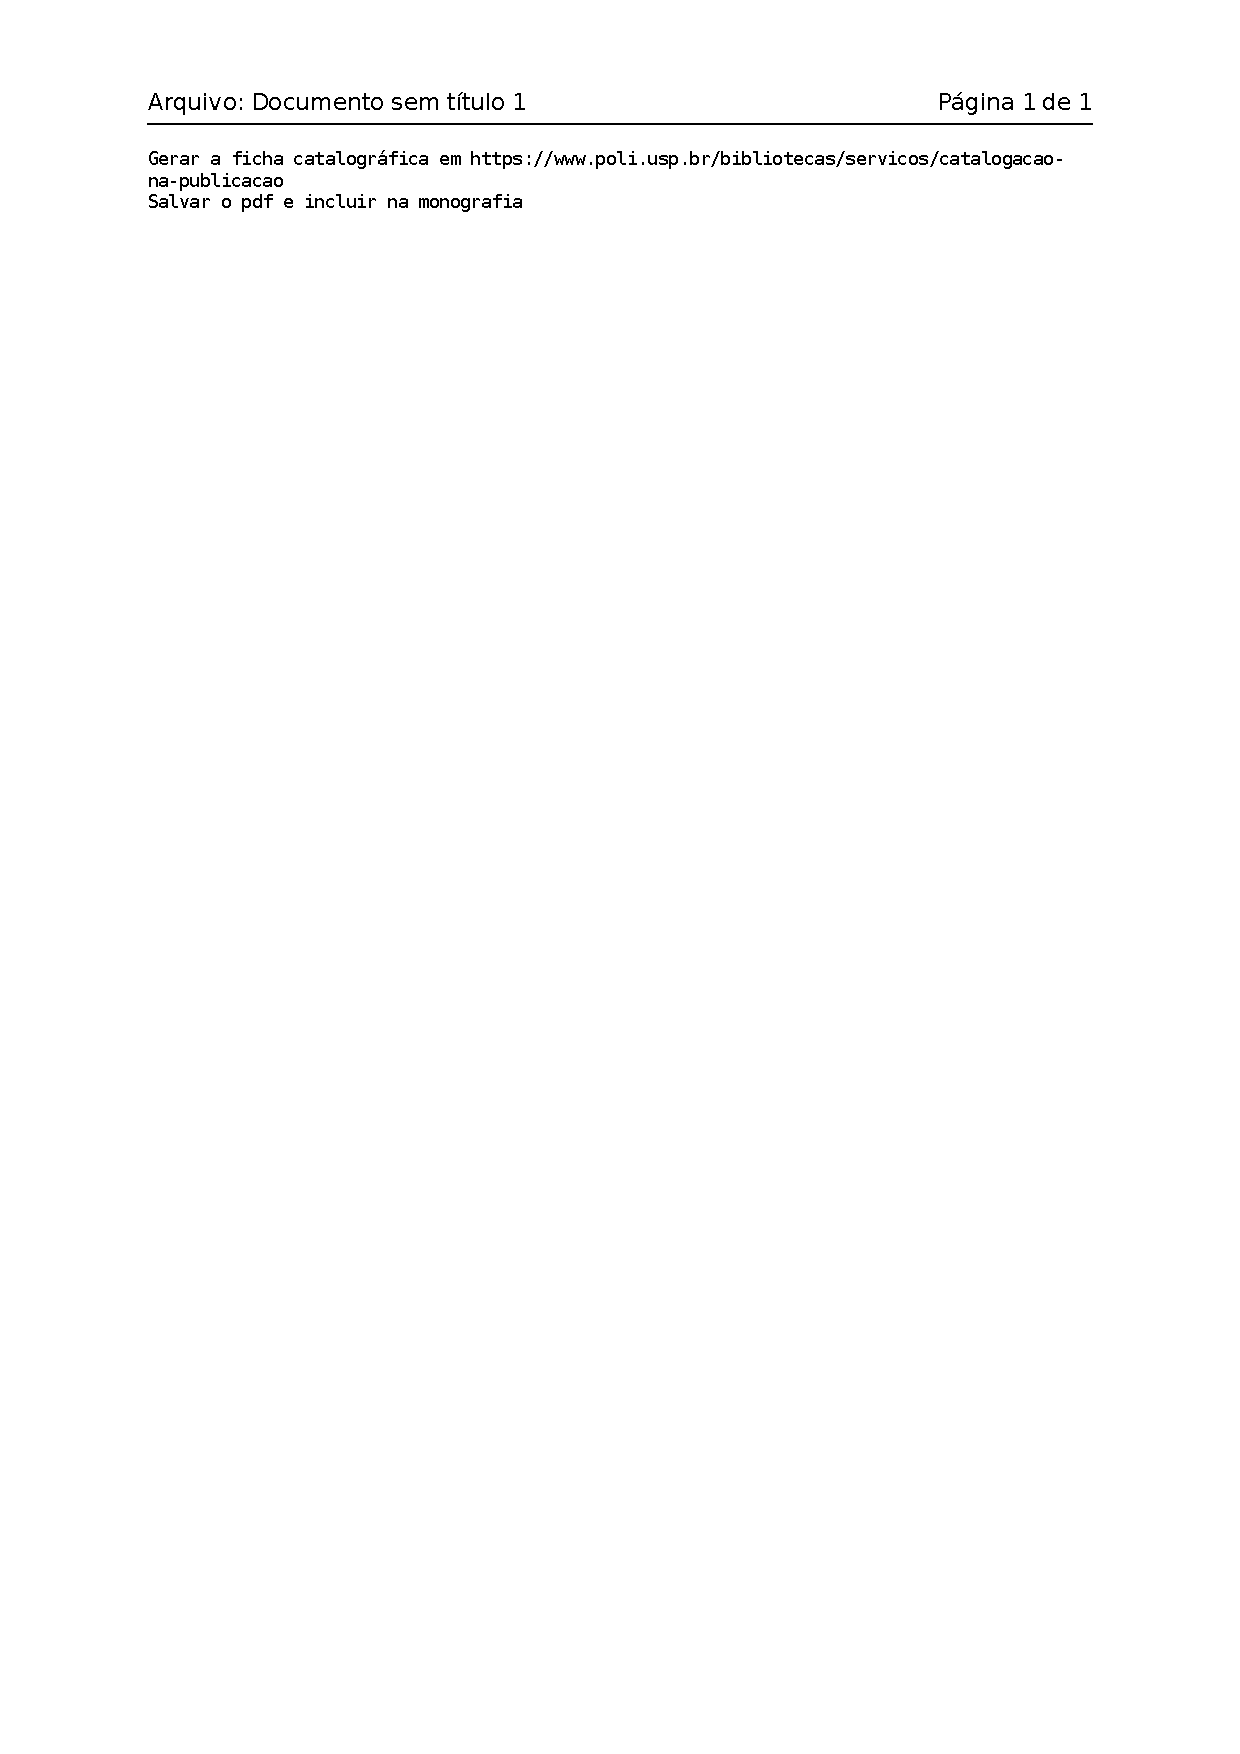
\includepdf{ficha.pdf}
 \hypersetup{pageanchor=true}
\end{fichacatalografica}

% \begin{fichacatalografica}
% 	\sffamily
% 	\vspace*{\fill}					% Posição vertical
% 	\begin{center}					% Minipage Centralizado
% 	\fbox{\begin{minipage}[c][8cm]{13.5cm}		% Largura
% 	\small
% 	\imprimirautor
% 	%Sobrenome, Nome do autor
	
% 	\hspace{0.5cm} \imprimirtitulo  / \imprimirautor. --
% 	\imprimirlocal, \imprimirdata-
	
% 	\hspace{0.5cm} \thelastpage p. : il. (algumas color.) ; 30 cm.\\
	
% 	\hspace{0.5cm} \imprimirorientadorRotulo~\imprimirorientador\\
	
% 	\hspace{0.5cm}
% 	\parbox[t]{\textwidth}{\imprimirtipotrabalho~--~\imprimirinstituicao,
% 	\imprimirdata.}\\
	
% 	\hspace{0.5cm}
% 		1. Palavra-chave1.
% 		2. Palavra-chave2.
% 		3. Palavra-chave3.
% 		I. Orientador.
% 		II. Universidade xxx.
% 		III. Faculdade de xxx.
% 		IV. Título 			
% 	\end{minipage}}
% 	\end{center}
% \end{fichacatalografica}
% ---

% ---
% Inserir errata
% ---
% \begin{errata}
% Elemento opcional da \citeonline[4.2.1.2]{NBR14724:2011}. Exemplo:

% \vspace{\onelineskip}

% FERRIGNO, C. R. A. \textbf{Tratamento de neoplasias ósseas apendiculares com
% reimplantação de enxerto ósseo autólogo autoclavado associado ao plasma
% rico em plaquetas}: estudo crítico na cirurgia de preservação de membro em
% cães. 2011. 128 f. Tese (Livre-Docência) - Faculdade de Medicina Veterinária e
% Zootecnia, Universidade de São Paulo, São Paulo, 2011.

% \begin{table}[htb]
% \center
% \footnotesize
% \begin{tabular}{|p{1.4cm}|p{1cm}|p{3cm}|p{3cm}|}
%   \hline
%    \textbf{Folha} & \textbf{Linha}  & \textbf{Onde se lê}  & \textbf{Leia-se}  \\
%     \hline
%     1 & 10 & auto-conclavo & autoconclavo\\
%    \hline
% \end{tabular}
% \end{table}

% \end{errata}
% ---

% ---
% Inserir folha de aprovação
% ---

% Isto é um exemplo de Folha de aprovação, elemento obrigatório da NBR
% 14724/2011 (seção 4.2.1.3). Você pode utilizar este modelo até a aprovação
% do trabalho. Após isso, substitua todo o conteúdo deste arquivo por uma
% imagem da página assinada pela banca com o comando abaixo:
%
% \begin{folhadeaprovacao}
% \includepdf{folhadeaprovacao_final.pdf}
% \end{folhadeaprovacao}
%
% \begin{folhadeaprovacao}

%   \begin{center}
%     {\ABNTEXchapterfont\large\imprimirautor}

%     \vspace*{\fill}\vspace*{\fill}
%     \begin{center}
%       \ABNTEXchapterfont\bfseries\Large\imprimirtitulo
%     \end{center}
%     \vspace*{\fill}
    
%     \hspace{.45\textwidth}
%     \begin{minipage}{.5\textwidth}
%         \imprimirpreambulo
%     \end{minipage}%
%     \vspace*{\fill}
%    \end{center}
        
%    Trabalho aprovado. \imprimirlocal, 24 de novembro de 2012:

%    \assinatura{\textbf{\imprimirorientador} \\ Orientador} 
%    \assinatura{\textbf{Professor} \\ Convidado 1}
%    \assinatura{\textbf{Professor} \\ Convidado 2}
%    %\assinatura{\textbf{Professor} \\ Convidado 3}
%    %\assinatura{\textbf{Professor} \\ Convidado 4}
      
%    \begin{center}
%     \vspace*{0.5cm}
%     {\large\imprimirlocal}
%     \par
%     {\large\imprimirdata}
%     \vspace*{1cm}
%   \end{center}
  
% \end{folhadeaprovacao}
% ---

% ---
% Dedicatória
% ---
\begin{dedicatoria}
   \vspace*{\fill}
   \centering
   \noindent
   \textit{Este trabalho é dedicado às crianças adultas que,\\
   quando pequenas, sonharam em se tornar cientistas.} \vspace*{\fill}
\end{dedicatoria}
% ---

% ---
% Agradecimentos
% ---
%\begin{agradecimentos}
%Os agradecimentos principais são direcionados ...

%\end{agradecimentos}
% ---

% ---
% Epígrafe
% ---
% \begin{epigrafe}
%     \vspace*{\fill}
% 	\begin{flushright}
% 		\textit{...}
% 	\end{flushright}
% \end{epigrafe}
% ---

% ---
% RESUMOS
% ---

% resumo em português
% O resumo deve ressaltar o  objetivo, o método, os resultados e as conclusões do documento. 
% Deve ser escrito em parágrafo única, e tipicamente é menor do que uma página.(\ldots) 
% As palavras-chave devem figurar logo abaixo do resumo, antecedidas da expressão Palavras-chave:, 
% separadas entre si por ponto e finalizadas também por ponto.
\setlength{\absparsep}{18pt} % ajusta o espaçamento dos parágrafos do resumo
\begin{resumo}
Redes de Internet das Coisas (IoT) baseadas em LoRa operam com dispositivos restritos em energia, memória e processamento, o que dificulta proteger os dados transmitidos e perceber comportamentos anômalos na rede. Este trabalho implementa e avalia um sistema de comunicação LoRa ponto a ponto, com o LoRaWAN como modelo de referência, que integra criptografia leve com o padrão Ascon e detecção de anomalias por aprendizado de máquina. Uma bancada própria, com nó sensor, \textit{gateway} e \textit{backend}, registra os metadados de recepção de cada quadro. A camada de segurança é uma biblioteca construída sobre uma implementação de código aberto do Ascon-128a, validada pelos vetores oficiais do algoritmo e por 4.907 adulterações de pacote, todas rejeitadas. Medido em dois microcontroladores ESP32, o Ascon-128a em \textit{software} cifra a mensagem típica de 23 bytes em 25 a 27~$\mu$s, sem alocação dinâmica de memória e com tempo de execução que não varia com os dados de entrada. O AES-128-GCM apoiado no acelerador de \textit{hardware} leva de 1,3 a 3,5 vezes esse tempo e gasta de 1,4 a 3,5 vezes a energia por operação. Na coleta de referência, o \textit{gateway} recebe 6.007 quadros protegidos pelo Ascon-128a em 8,3 horas, sem perda de rádio e sem rejeição. A detecção de anomalias é especificada como regressão temporal, com modelos ARIMA, RNN e LSTM ajustados ao tráfego normal de um conjunto de dados público, em que o desvio entre o valor previsto e o observado indica a anomalia. Os resultados mostram que a criptografia leve em \textit{software} dispensa o acelerador de \textit{hardware} nos pacotes pequenos típicos dessas redes, e que o custo de proteger o enlace está nos bytes acrescentados a cada mensagem, e não no processamento.

 \textbf{Palavras-chave}: LoRaWAN. Internet das Coisas. Criptografia leve. Ascon. Detecção de anomalias.
\end{resumo}
\begin{resumo}[Abstract]
 \begin{otherlanguage*}{english}
   Internet of Things (IoT) networks based on LoRa rely on devices with limited energy, memory and processing power, which makes it hard to protect transmitted data and to notice anomalous network behavior. This work implements and evaluates a point-to-point LoRa communication system, with LoRaWAN as the reference model, that integrates lightweight cryptography with the Ascon standard and anomaly detection by machine learning. A purpose-built test bench, with a sensor node, a gateway and a backend, records the reception metadata of every frame. The security layer is a library built on an open-source implementation of Ascon-128a, validated against the official test vectors of the algorithm and against 4,907 packet tampering cases, all of them rejected. Measured on two ESP32 microcontrollers, Ascon-128a in software encrypts the typical 23-byte message in 25 to 27~$\mu$s, with no dynamic memory allocation and with an execution time that does not vary with the input data. AES-128-GCM backed by the hardware accelerator takes 1.3 to 3.5 times as long and uses 1.4 to 3.5 times the energy per operation. In the reference collection, the gateway receives 6,007 frames protected by Ascon-128a in 8.3 hours, with no radio loss and no rejection. Anomaly detection is specified as temporal regression, with ARIMA, RNN and LSTM models fitted to the normal traffic of a public dataset, in which the deviation between the predicted and the observed value indicates the anomaly. The results show that lightweight cryptography in software makes the hardware accelerator unnecessary for the small packets typical of these networks, and that the cost of protecting the link lies in the bytes added to each message, not in processing.

   \vspace{\onelineskip}
 
   \noindent 
   \textbf{Keywords}: LoRaWAN. Internet of Things. Lightweight cryptography. Ascon. Anomaly detection.
 \end{otherlanguage*}
\end{resumo}
% \begin{resumo}[Résumé]
%  \begin{otherlanguage*}{french}
%     Il s'agit d'un résumé en français.
 
%    \textbf{Mots-clés}: latex. abntex. publication de textes.
%  \end{otherlanguage*}
% \end{resumo}

% % resumo em espanhol
% \begin{resumo}[Resumen]
%  \begin{otherlanguage*}{spanish}
%    Este es el resumen en español.
  
%    \textbf{Palabras clave}: latex. abntex. publicación de textos.
%  \end{otherlanguage*}
% \end{resumo}
% ---

% ---
% inserir lista de ilustrações
% ---
\pdfbookmark[0]{\listfigurename}{lof}
\listoffigures*
\cleardoublepage
% ---

% ---
% inserir lista de quadros
% ---
\pdfbookmark[0]{\listofquadrosname}{loq}
\listofquadros*
\cleardoublepage
% ---

% ---
% inserir lista de tabelas
% ---
\pdfbookmark[0]{\listtablename}{lot}
\listoftables*
\cleardoublepage
% ---

% ---
% inserir lista de abreviaturas e siglas
% ---
\begin{siglas}
  \item[ABNT] Associação Brasileira de Normas Técnicas
  \item[ABP] Activation by Personalization
  \item[AD] Associated Data
  \item[ADR] Adaptive Data Rate
  \item[AEAD] Authenticated Encryption with Associated Data
  \item[AES] Advanced Encryption Standard
  \item[ANATEL] Agência Nacional de Telecomunicações
  \item[API] Application Programming Interface
  \item[ARIMA] AutoRegressive Integrated Moving Average
  \item[BW] Bandwidth
  \item[CAESAR] Competition for Authenticated Encryption: Security, Applicability, and Robustness
  \item[CMAC] Cipher-based Message Authentication Code
  \item[CPU] Central Processing Unit
  \item[CR] Coding Rate
  \item[CRC] Cyclic Redundancy Check
  \item[CSS] Chirp Spread Spectrum
  \item[CSV] Comma-Separated Values
  \item[CTR] Counter Mode
  \item[CXOF128] Customizable Extendable-Output Function, 128-bit
  \item[DDoS] Distributed Denial of Service
  \item[DES] Data Encryption Standard
  \item[DMA] Direct Memory Access
  \item[DoS] Denial of Service
  \item[DRBG] Deterministic Random Bit Generator
  \item[ED] End Device
  \item[ESP-IDF] Espressif IoT Development Framework
  \item[ESP32] Espressif 32
  \item[ETL] Extract, Transform, Load
  \item[FCnt] Frame Counter
  \item[FOpts] Frame Options
  \item[FPGA] Field-Programmable Gate Array
  \item[FPort] Frame Port
  \item[GCM] Galois/Counter Mode
  \item[GHASH] Galois Hash
  \item[GPIO] General-Purpose Input/Output
  \item[HTTP] Hypertext Transfer Protocol
  \item[IDE] Integrated Development Environment
  \item[IoT] Internet of Things
  \item[IP] Internet Protocol
  \item[ISO/IEC] International Organization for Standardization / International Electrotechnical Commission
  \item[IV] Initialization Vector
  \item[JSON] JavaScript Object Notation
  \item[KAT] Known Answer Tests
  \item[LDO] Low-Dropout Regulator
  \item[LED] Light-Emitting Diode
  \item[LoRa] Long Range
  \item[LoRaWAN] Long Range Wide Area Network
  \item[LPWAN] Low-Power Wide-Area Network
  \item[LSTM] Long Short-Term Memory
  \item[MAC] Medium Access Control, na camada de enlace, e Message Authentication Code, na autenticação de mensagens
  \item[MAE] Mean Absolute Error
  \item[MIC] Message Integrity Code
  \item[MitM] Man-in-the-Middle
  \item[ML] Machine Learning
  \item[NIST] National Institute of Standards and Technology
  \item[NTP] Network Time Protocol
  \item[NVS] Non-Volatile Storage
  \item[OTAA] Over-the-Air Activation
  \item[OTP] One-Time Programmable
  \item[PHY] Physical Layer
  \item[RAM] Random Access Memory
  \item[RBG] Random Bit Generator
  \item[RF] Rádio Frequência
  \item[RM-ODP] Reference Model of Open Distributed Processing
  \item[RMSE] Root Mean Squared Error
  \item[RNN] Recurrent Neural Network
  \item[RSSI] Received Signal Strength Indicator
  \item[SF] Spreading Factor
  \item[SIV] Synthetic Initialization Vector
  \item[SNR] Signal-to-Noise Ratio
  \item[SPI] Serial Peripheral Interface
  \item[TCXO] Temperature-Compensated Crystal Oscillator
  \item[TinyML] Tiny Machine Learning
  \item[TRNG] True Random Number Generator
  \item[UML] Unified Modeling Language
  \item[USB] Universal Serial Bus
  \item[UTC] Coordinated Universal Time
  \item[XOF128] Extendable-Output Function, 128-bit
\end{siglas}
% ---

% ---
% inserir lista de símbolos
% ---
\begin{simbolos}
  \item[$\mathrm{BW}$] Largura de banda do canal LoRa
  \item[$\mathrm{CR}$] Taxa de codificação do enlace LoRa
  \item[$\mathrm{CRC}$] Indicador de habilitação do código de verificação cíclica
  \item[$\mathrm{DE}$] Indicador de habilitação da otimização para baixas taxas de dados
  \item[$\mathrm{IH}$] Indicador de omissão do cabeçalho físico
  \item[$K$] Chave criptográfica
  \item[$\lambda$] Tamanho da \textit{tag} de autenticação, em bits
  \item[$n$] Número de observações no conjunto de teste
  \item[$n_{\mathrm{payload}}$] Número de símbolos do \textit{payload} LoRa
  \item[$n_{\mathrm{pre}}$] Número de símbolos do preâmbulo LoRa
  \item[$\mathrm{PL}$] Comprimento do \textit{payload}, em bytes
  \item[$\mathrm{SF}$] Fator de espalhamento do enlace LoRa
  \item[$T_{\mathrm{pacote}}$] Tempo no ar do pacote LoRa
  \item[$T_{\mathrm{pre}}$] Duração do preâmbulo LoRa
  \item[$T_s$] Duração de um símbolo LoRa
  \item[$U$] Sequência de bits extraída do gerador aleatório aprovado
  \item[$V$] Sequência de bits independente usada na derivação da chave
  \item[$y_i$] Valor observado na posição $i$
  \item[$\hat{y}_i$] Valor previsto pelo modelo na posição $i$
  \item[$i$] Índice de uma observação
  \item[$\Delta$] Diferença entre o consumo durante o processamento e a corrente de repouso
  \item[$\oplus$] Operação XOR (ou-exclusivo)
  \item[$\leq$] Relação menor ou igual
\end{simbolos}
% ---

% ---
% inserir o sumario
% ---
\pdfbookmark[0]{\contentsname}{toc}
\tableofcontents*
\cleardoublepage
% ---


% ----------------------------------------------------------
% ELEMENTOS TEXTUAIS
% ----------------------------------------------------------
\hypersetup{pageanchor=true}
\textual

% Capítulo 1. Introdução
\chapter{Introdução} \label{cap:introducao}

A Internet das Coisas (IoT) é composta por dispositivos embarcados que desempenham funções específicas, atuando como sensores e controladores para uma variedade de aplicações tecnológicas produzidas hoje em dia, desde os aparelhos mais simples do cotidiano até processos industriais complexos. Com a evolução do hardware, os dispositivos IoT tornaram-se menores, mais rápidos, mais eficientes e com menor custo, o que levou a uma explosão do seu uso \cite{alfuqaha2015iot}.

Contudo, um dos principais entraves para essa tecnologia decorre das limitações energéticas e computacionais desses dispositivos \cite{nistir8114}. Apesar da evolução vista nas últimas décadas, a IoT ainda enfrenta gargalos em processos que demandam alto poder computacional, devido à grande carga de processamento e ao elevado custo energético.

Diante desse cenário, surgem questões de segurança que podem ser exploradas para invadir e comprometer o funcionamento da rede. Para resolver a questão da transmissão segura e eficiente, ganham relevância padrões como o Ascon, motivados pela necessidade de padronizar um conjunto de métodos criptográficos leves, adequados a dispositivos com baixo consumo energético \cite{nist800232}. Em paralelo, para viabilizar a comunicação de longa distância com baixa energia, utiliza-se amplamente o protocolo LoRaWAN, que possui aplicações fundamentais em diversas áreas, desde a infraestrutura de cidades inteligentes e controle de tráfego até o monitoramento de desastres, agricultura de precisão e automação industrial com foco em manutenção preditiva. O grande problema enfrentado por esse protocolo, no entanto, é a segurança da informação frente a ataques como \textit{jamming}, \textit{replay attacks}, \textit{spoofing} e \textit{denial of service} \cite{hessel2023lorawan}. A vulnerabilidade a ataques pode causar disrupções críticas e prejuízos severos, tornando indispensável a aplicação de métodos robustos de prevenção. 

%%%%%%%%%%%%%%%%%%%%%%%%%%%%%%%%%%%%%%%%%%%%%%%%%%%%
%%%%%%%%%%%%%%%%%%%%%%%%%%%%%%%%%%%%%%%%%%%%%%%%%%%%

\section{Motivação}
A necessidade de operar com baixo consumo energético eleva bastante a complexidade do uso de dispositivos IoT, uma vez que tentativas de mitigar esse problema podem resultar em simplificações que geram problemas de segurança \cite{nistir8114, hessel2023lorawan}. Diante disso, torna-se pertinente compreender a natureza desses ataques e suas formas de mitigação, além de estudar a eficiência e a eficácia de modelos de Machine Learning na detecção de intrusões e anomalias.

Um desses problemas é a vulnerabilidade a ataques diretos, como ataques de negação de serviço (DoS) ou \textit{jamming}, que podem esgotar a bateria do dispositivo ou impedir que a coleta de dados seja feita de maneira adequada \cite{hessel2023lorawan}. Outro grande desafio está na comunicação: é preciso garantir que a informação transmitida entre os dispositivos não possa ser interceptada nem modificada, assegurando a integridade, confidencialidade e autenticidade dos dados. Como os algoritmos de segurança comumente utilizados foram concebidos para plataformas de propósito geral, torna-se necessário buscar maneiras mais eficientes de proteger os dados durante a transmissão \cite{nistir8114}.


O uso de \textit{Machine Learning} neste trabalho decorre da necessidade de 
detectar anomalias em redes LoRaWAN a partir de padrões temporais e 
comportamentais dos dados. Em contextos reais de IoT, abordagens baseadas 
apenas em regras fixas ou limiares estáticos tendem a ser limitadas. O 
comportamento normal pode variar conforme o contexto operacional (dispositivo, 
gateway, ambiente) e evoluir ao longo do tempo, tornando limiares fixos 
(ex: ``se RSSI < -120 dBm, alertar'') inadequados. Além disso, métodos 
tradicionais apresentam dificuldade em capturar estruturas complexas em dados 
sequenciais, tais como degradação gradual de equipamento ou padrões não 
lineares de transmissão. Por outro lado, abordagens baseadas em aprendizado 
conseguem modelar relações temporais, identificar desvios sutis e adaptar-se 
dinamicamente à evolução do comportamento normal, mostrando-se mais adequadas 
para este contexto \cite{chalapathy2019}.

Por isso, a modelagem é realizada com base no comportamento esperado do dispositivo em suas circunstâncias normais de operação, buscando aprender padrões legítimos de funcionamento a partir dos dados observados. Nessa abordagem, desvios suficientemente relevantes em relação ao comportamento previamente aprendido são tratados como indícios de anomalia. Trata-se, portanto, de uma abordagem adaptativa, pois o modelo se ajusta ao perfil comportamental de cada nó monitorado. \cite{hayashi2022handsfree}.


Assim, neste trabalho, \textit{Machine Learning} é tratado como um dos núcleos centrais da investigação. Seu papel não é apenas classificar dados, mas aprender perfis de operação, comparar abordagens de detecção e oferecer uma base experimental para uma etapa posterior de avaliação em borda. Essa decisão amplia o escopo da análise, permitindo estudar simultaneamente eficácia de detecção, robustez metodológica e viabilidade de implantação em borda.

O padrão Ascon, por sua vez, foi selecionado para padronização ao final da competição de criptografia leve do NIST \cite{nistir8454}, tendo sido também a primeira escolha para criptografia leve no portfólio final da competição CAESAR \cite{caesar_submissions}. A relevância desse padrão se torna clara quando se analisa sua eficiência em software e hardware, particularmente em dispositivos restritos, reunindo confidencialidade, integridade e autenticidade em uma única operação (AEAD) e facilitando a proteção contra ataques de canal colateral \cite{ascon_official}.

A avaliação dessas duas frentes exige dados de rede obtidos em condições controladas. Conjuntos de dados públicos registram a operação de redes reais, mas não permitem controlar as duas pontas do enlace nem reproduzir uma condição específica de operação. Por isso, o trabalho constrói também uma bancada própria de comunicação LoRa, sobre a qual a camada criptográfica e os modelos de detecção são avaliados.


%%%%%%%%%%%%%%%%%%%%%%%%%%%%%%%%%%%%%%%%%%%%%%%%%%%%
%%%%%%%%%%%%%%%%%%%%%%%%%%%%%%%%%%%%%%%%%%%%%%%%%%%%

\section{Objetivos}
O objetivo geral deste trabalho é implementar e avaliar um sistema de comunicação LoRa ponto a ponto, tendo o LoRaWAN como modelo de referência, integrando a aplicação de modelos de \textit{Machine Learning} e o padrão de criptografia leve Ascon. A finalidade central é analisar o nível de segurança e a resiliência que a combinação dessas duas tecnologias pode oferecer ao ecossistema de Internet das Coisas (IoT).

Para o alcance do objetivo geral, foram definidos os seguintes objetivos específicos:

\begin{itemize}
    \item Construir e validar uma infraestrutura de comunicação LoRa ponto a ponto, composta por nó sensor, \textit{gateway} e \textit{backend}, que registre os metadados de recepção de cada quadro.
    \item Treinar e testar modelos de \textit{Machine Learning}, utilizando os \textit{datasets} selecionados, para atuar na identificação e mitigação de ameaças ativas, tais como \textit{jamming}, \textit{spoofing} e ataques de Negação de Serviço (DoS).
    \item Integrar ao nó sensor uma implementação do algoritmo Ascon e desenvolver sobre ela uma camada de segurança que garanta a confidencialidade, a autenticidade e a integridade dos dados transmitidos, com baixo custo computacional.
    \item Desenvolver o protótipo do sistema integrando as camadas de comunicação, de criptografia e de detecção
    \item Analisar o nível de segurança global oferecido pelo conjunto, validando a eficácia da solução proposta frente às restrições do hardware, em termos de latência, memória e consumo energético.
\end{itemize}

%%%%%%%%%%%%%%%%%%%%%%%%%%%%%%%%%%%%%%%%%%%%%%%%%%%%
%%%%%%%%%%%%%%%%%%%%%%%%%%%%%%%%%%%%%%%%%%%%%%%%%%%%

\section{Justificativa}
A relevância deste trabalho evidencia-se pelo papel central e pela rápida expansão dos dispositivos de Internet das Coisas (IoT) no cotidiano, com projeções indicando dezenas de bilhões de equipamentos conectados nos próximos anos \cite{ericsson2026mobility}. Propor uma metodologia que integra tecnologias e conceitos críticos como a comunicação LoRa de longo alcance e baixo consumo, tendo o LoRaWAN como referência, modelos de \textit{Machine Learning} e segurança criptográfica, e verificar a sua eficácia em cenários práticos, demonstra como a união dessas ferramentas pode alavancar a resiliência de sistemas reais, tornando-os cada vez mais robustos contra ameaças.

%%%%%%%%%%%%%%%%%%%%%%%%%%%%%%%%%%%%%%%%%%%%%%%%%%%%
%%%%%%%%%%%%%%%%%%%%%%%%%%%%%%%%%%%%%%%%%%%%%%%%%%%%

\section{Organização do Trabalho}
Para facilitar a leitura e a compreensão da pesquisa, este documento está estruturado da seguinte forma:

O Capítulo \ref{cap:conceitos} apresenta os aspectos conceituais que fundamentam o projeto. Nele, são abordados a camada física LoRa, o funcionamento do protocolo LoRaWAN, adotado como modelo de referência, e o paradigma da criptografia leve (\textit{Lightweight Cryptography}), detalhando o processo de padronização do NIST que elegeu a família Ascon, além de uma comparação com outras famílias de algoritmos. O capítulo também explora a base teórica de \textit{Machine Learning} voltada para a detecção de anomalias.

O Capítulo \ref{cap:metodo} descreve o método do trabalho. Primeiramente, apresenta-se a abordagem de elicitação de requisitos adotada, incluindo análise de literatura, identificação de restrições de hardware e validação de viabilidade técnica. Descrevem-se ainda os materiais e o protocolo de coleta adotados na avaliação do enlace LoRa. Em seguida, são detalhados os datasets analisados e selecionados para o modelo de Machine Learning, os procedimentos de treinamento e avaliação, bem como a justificativa para a adoção da biblioteca ascon-suite na implementação do padrão Ascon. O capítulo abrange 
ainda as etapas de configuração do ambiente, implementação e métodos de teste.

O Capítulo \ref{cap:especificacao} trata da especificação da arquitetura do sistema e de seus requisitos, os funcionais e não funcionais da infraestrutura, os do sistema de detecção de anomalias e os de segurança da camada criptográfica, que o protótipo deve respeitar para operar na borda da rede.

O Capítulo \ref{cap:desenvolvimento} é dedicado ao projeto e desenvolvimento. Nesta etapa, são descritas as tecnologias e ferramentas práticas utilizadas, a arquitetura montada, a infraestrutura de comunicação implementada, os testes realizados e a discussão dos resultados obtidos, incluindo os resultados de operação do enlace.

Por fim, o Capítulo \ref{cap:consideracoes} apresenta as considerações finais, com as conclusões extraídas da pesquisa, as contribuições da equipe e os direcionamentos para futuras implementações e melhorias que podem surgir a partir deste trabalho.


% Capítulo 2. Aspectos Conceituais
\chapter{Aspectos Conceituais} \label{cap:conceitos}


A proteção efetiva de um sistema não é alcançada por uma única técnica, 
mas pela combinação de estratégias em múltiplas camadas. Conforme o 
\textit{NIST Cybersecurity Framework} \cite{nist_csf_2024}, a segurança 
robusta exige tanto \textbf{prevenção} (impedindo que ataques ocorram) 
quanto \textbf{detecção} (identificando atividades suspeitas). Este 
capítulo apresenta os conceitos que fundamentam este trabalho dentro 
desse paradigma: protocolos de comunicação para IoT, criptografia leve 
como mecanismo preventivo, e Machine Learning como mecanismo de detecção 
comportamental.


\section{Redes IoT e o Protocolo LoRaWAN}

As redes de Internet das Coisas (IoT) utilizam amplamente o protocolo LoRaWAN em cenários que exigem baixo consumo de energia e ampla cobertura. Embora o LoRaWAN apresente certa maturidade e conte com mecanismos de proteção continuamente aprimorados, ataques e problemas de segurança ainda afetam sua resiliência. Consequentemente, permanece necessária a evolução contínua de técnicas de prevenção e mitigação dessas ameaças \cite{hessel2023lorawan}.

%%%%%%%%%%%%%%%%%%%%%%%%%%%%%%%%%%%%%%%%%%%%%%%%%%%%

\subsection{LoRa e LoRaWAN: fundamentos e evolução do protocolo}

O LoRaWAN se destaca como uma tecnologia voltada a redes LPWAN (\textit{Low-Power Wide-Area Network}), sendo utilizado em aplicações como monitoramento remoto, agricultura inteligente e sistemas distribuídos com dispositivos embarcados. Sua proposta é permitir a comunicação entre dispositivos com baixo consumo energético, ampla cobertura e custo operacional reduzido.

É importante distinguir os termos \textit{LoRa} e \textit{LoRaWAN}, que frequentemente são tratados como sinônimos, embora representem camadas diferentes da tecnologia. O LoRa corresponde à camada física da comunicação, isto é, à técnica de modulação empregada no enlace sem fio. Já o LoRaWAN define o protocolo de comunicação acima dessa camada, estabelecendo regras para organização da rede, troca de mensagens e controle da comunicação. Em outras palavras, o LoRa fornece o meio de transmissão por rádio, enquanto o LoRaWAN define o funcionamento da rede sobre esse meio.

De forma geral, o LoRaWAN foi projetado para redes compostas por dispositivos com recursos limitados, muitas vezes alimentados por bateria e instalados em locais de difícil manutenção. Por isso, o protocolo prioriza simplicidade operacional, baixo consumo e comunicação eficiente, ainda que com taxas de transmissão menores do que tecnologias voltadas a maior vazão de dados. Essa característica o torna adequado para cenários em que pequenas quantidades de informação precisam ser transmitidas periodicamente, sem necessidade de comunicação contínua.

A evolução do LoRaWAN também é um aspecto importante. Desde sua primeira publicação, em 2015, o protocolo passou por revisões que resultaram em dois ramos principais: a família 1.0.x e a versão 1.1. As versões da família 1.0.x mantiveram interoperabilidade entre si e trouxeram principalmente correções, esclarecimentos e ajustes incrementais. Já a versão 1.1 introduziu mudanças mais relevantes, especialmente na organização de funções da rede e nos mecanismos de segurança, tornando mais clara a separação entre responsabilidades de rede e de aplicação. Neste trabalho, adota-se a família 1.0.x, uma vez que os dados utilizados na frente de aprendizado de máquina provêm de redes nas versões 1.0.3 e 1.0.4. Essa família é adotada como modelo de referência: a implementação deste trabalho utiliza a camada física LoRa em um enlace ponto a ponto, e reproduz da especificação LoRaWAN 1.0.4 \cite{lorawan104}.


\begin{figure}[htb]
  \caption{\label{lorawan_version_history}Histórico de versionamento da especificação da LoRaWAN}
  \begin{center}
      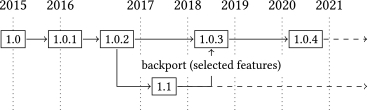
\includegraphics[scale=0.8]{barea/figuras/lorawan_version_history.png}
  \end{center}
  \legend{Fonte: \cite{hessel2023lorawan}}
\end{figure}

Mesmo com a introdução de melhorias nas versões mais recentes, a adoção de novas revisões do protocolo não ocorre de forma imediata em sistemas reais. Em aplicações IoT, sensores podem permanecer em operação por muitos anos, frequentemente sem atualização de firmware. Como consequência, versões anteriores do LoRaWAN continuam relevantes na prática, e essa coexistência entre gerações do protocolo precisa ser considerada em qualquer análise técnica ou experimental.

Assim, compreender a distinção entre LoRa e LoRaWAN, bem como a evolução do protocolo ao longo de suas versões, é essencial para analisar corretamente seu funcionamento em sistemas embarcados conectados. A partir dessa base, as próximas subseções detalham a arquitetura da rede, o processo de ativação dos dispositivos, a transferência de dados, os mecanismos de gerenciamento da comunicação e a relação dessas tecnologias com a arquitetura proposta neste trabalho.

%%%%%%%%%%%%%%%%%%%%%%%%%%%%%%%%%%%%%%%%%%%%%%%%%%%%

\subsection{A camada física LoRa}
\label{subsec:camada_fisica_lora}

O LoRa é uma técnica de modulação proprietária da Semtech, baseada em espalhamento espectral por \textit{chirp} (\textit{Chirp Spread Spectrum}, CSS). Cada símbolo é um \textit{chirp}, um sinal cuja frequência varre linearmente toda a largura de banda do canal, e a informação é codificada no instante em que essa varredura se inicia. Como a energia do símbolo é distribuída por toda a banda durante um intervalo relativamente longo, o receptor consegue correlacionar o sinal recebido com o padrão esperado mesmo quando a potência do sinal está abaixo do piso de ruído. É essa propriedade que permite sensibilidades da ordem de $-130$~dBm e enlaces de quilômetros com potências de transmissão de poucas dezenas de miliwatts \cite{semtech2015sx1276}.

Três parâmetros definem o comportamento de um enlace LoRa. O fator de espalhamento (\textit{Spreading Factor}, SF), de 7 a 12, determina quantos \textit{chirps} compõem um símbolo ($2^{\mathrm{SF}}$): cada incremento de SF dobra a duração do símbolo, aumenta a sensibilidade do receptor em cerca de 2,5~dB e reduz a taxa de dados pela metade. A largura de banda (BW), tipicamente 125, 250 ou 500~kHz, define a velocidade da varredura: bandas mais largas transmitem mais rápido e são menos sensíveis. A taxa de codificação (\textit{Coding Rate}, CR), de 4/5 a 4/8, acrescenta redundância de correção de erros ao custo de mais bits transmitidos. A Tabela~\ref{tab:parametros_lora} resume o efeito de cada parâmetro. A combinação de SF e BW define a taxa de dados (\textit{data rate}), e o LoRaWAN numera essas combinações em índices DR0 a DR6, em que DR0 corresponde à combinação mais lenta e de maior alcance.

\begin{table}[htb]
\centering
\caption{Efeito dos parâmetros da modulação LoRa}
\label{tab:parametros_lora}
\begin{tabular}{llll}
\hline
\textbf{Parâmetro} & \textbf{Ao aumentar} & \textbf{Ganha} & \textbf{Perde} \\
\hline
SF (7-12)   & 2x o tempo & sensibilidade, alcance & dados, energia/quadro \\
BW (125-500 kHz) & acelera varredura & dados & sensibilidade \\
CR (4/5-4/8) & redundância & robustez a erros & taxa útil \\
\hline
\end{tabular}
\legend{Fonte: elaborado a partir de \cite{semtech2015sx1276}.}
\end{table}

A consequência direta desses parâmetros é o tempo no ar (\textit{time on air}) de cada pacote, isto é, o intervalo durante o qual o transmissor ocupa o canal. O datasheet do transceptor \cite{semtech2015sx1276} fornece a fórmula: o tempo de símbolo é $T_s = 2^{\mathrm{SF}}/\mathrm{BW}$; o preâmbulo dura $T_{\mathrm{pre}} = (n_{\mathrm{pre}} + 4{,}25)\,T_s$, em que $n_{\mathrm{pre}}$ é o número de símbolos de preâmbulo programado; e o número de símbolos do payload é dado pela Equação~\ref{eq:npayload},

\begin{equation}
\label{eq:npayload}
n_{\mathrm{payload}} = 8 + \max\!\left( \left\lceil \frac{8\,\mathrm{PL} - 4\,\mathrm{SF} + 28 + 16\,\mathrm{CRC} - 20\,\mathrm{IH}}{4\,(\mathrm{SF} - 2\,\mathrm{DE})} \right\rceil (\mathrm{CR} + 4),\; 0 \right),
\end{equation}

\noindent em que PL é o número de bytes do payload, CRC vale 1 quando o código de verificação está habilitado, IH vale 1 quando o cabeçalho físico é omitido e DE vale 1 quando a otimização para baixas taxas (\textit{LowDataRateOptimize}) está ativa, o que o fabricante exige sempre que o tempo de símbolo ultrapassa 16~ms. O tempo no ar do pacote é $T_{\mathrm{pacote}} = T_{\mathrm{pre}} + n_{\mathrm{payload}}\,T_s$. Como $T_s$ dobra a cada incremento de SF, um mesmo pacote leva aproximadamente 25 vezes mais tempo no ar em SF12 do que em SF7. O tempo no ar determina a energia gasta por transmissão, a ocupação do canal e o tempo de exposição do quadro a interferência, e por isso é a grandeza que orienta a escolha dos parâmetros neste trabalho, apresentada no Capítulo~\ref{cap:metodo}.

O tamanho do payload é limitado em dois níveis. O campo de comprimento do pacote LoRa tem 8~bits, o que impõe o máximo físico de 255~bytes. Acima dele, os parâmetros regionais do LoRaWAN \cite{lorawan_rp002} limitam o payload de aplicação por taxa de dados, para conter o tempo no ar nas taxas mais lentas: no plano AU915, adotado no Brasil, o limite em DR0 é de 51~bytes. Um quadro que respeite esse limite pode ser transmitido em qualquer SF, inclusive nos de maior alcance.

Dois indicadores medidos pelo receptor a cada pacote descrevem a qualidade do enlace. O RSSI (\textit{Received Signal Strength Indicator}), em dBm, é a potência do sinal recebido, incluindo o ruído; valores mais próximos de zero indicam sinal mais forte. O SNR (\textit{Signal-to-Noise Ratio}), em dB, é a razão entre a potência do sinal e a do ruído; o LoRa opera com SNR negativo, até cerca de $-20$~dB em SF12, o que é justamente o que o espalhamento espectral torna possível. Em enlaces curtos e com sinal forte, o estimador de SNR do transceptor satura em torno de $+10$ a $+13$~dB e o valor deixa de variar, de modo que o SNR só se torna informativo à medida que o enlace se aproxima do seu limite de alcance. Esses dois indicadores, junto com o contador de quadros e o intervalo entre chegadas, são metadados de recepção: são produzidos pelo receptor e não dependem do conteúdo transmitido, o que os torna observáveis mesmo quando o payload é cifrado.

O LoRa opera em faixas de uso livre abaixo de 1~GHz, que variam por região. No Brasil, a ANATEL autoriza equipamentos de radiação restrita com modulação digital nas faixas de 902 a 907,5~MHz e de 915 a 928~MHz, sem necessidade de licença \cite{anatel_radiacao_restrita}. A essa segunda faixa corresponde o plano regional AU915 do LoRaWAN \cite{lorawan_rp002}, que a divide em 64 canais de \textit{uplink} de 125~kHz agrupados em oito sub-bandas, mais oito canais de 500~kHz.

Por fim, é preciso registrar o que a camada física não oferece. O LoRa define apenas a modulação e a estrutura do pacote: preâmbulo, cabeçalho físico opcional, payload e um código de verificação (CRC) de 16~bits. Não há endereçamento, controle de acesso ao meio nem qualquer mecanismo de segurança. O CRC detecta erros de transmissão, mas pode ser recalculado por qualquer parte, e portanto não protege contra modificação, forja ou repetição de quadros. No LoRaWAN, essas funções são acrescentadas pela camada MAC, que define endereços, contadores e a proteção criptográfica do quadro com AES-128 no modo CTR para confidencialidade e AES-CMAC para o código de integridade \cite{lorawan104}. Em um enlace que utilize apenas a camada física LoRa, tudo o que está acima dela precisa ser fornecido pela aplicação. Essa constatação fundamenta a arquitetura adotada neste trabalho, discutida na Subseção~\ref{subsec:implicacoes_arquitetura}.


%%%%%%%%%%%%%%%%%%%%%%%%%%%%%%%%%%%%%%%%%%%%%%%%%%%%

\subsection{Arquitetura da Rede}

A arquitetura do LoRaWAN é composta por diferentes entidades, cada uma com uma função específica no funcionamento da rede. De forma geral, os dispositivos finais, chamados de \textit{End Devices}, são responsáveis por coletar e transmitir dados. Esses dispositivos se comunicam por rádio com um ou mais \textit{Gateways}, que atuam como pontes entre a rede LoRa e a infraestrutura conectada por IP. Os gateways, por sua vez, apenas recebem os quadros transmitidos pelos dispositivos e os encaminham para os servidores da rede, sem realizar processamento completo do protocolo. \cite{hessel2023lorawan}

Essa organização forma uma topologia conhecida como \textit{star-of-stars}. Nela, os dispositivos finais não se comunicam diretamente entre si, e também não estabelecem vínculo fixo com um único gateway. Em vez disso, uma mesma transmissão pode ser recebida por vários gateways que estejam dentro de alcance. Essa característica aumenta a cobertura da rede e oferece maior robustez na recepção das mensagens, especialmente em cenários distribuídos e com mobilidade.

\begin{figure}[htb]
  \caption{\label{lorawan_architeture}Arquitetura de rede LoRaWAN}
  \begin{center}
      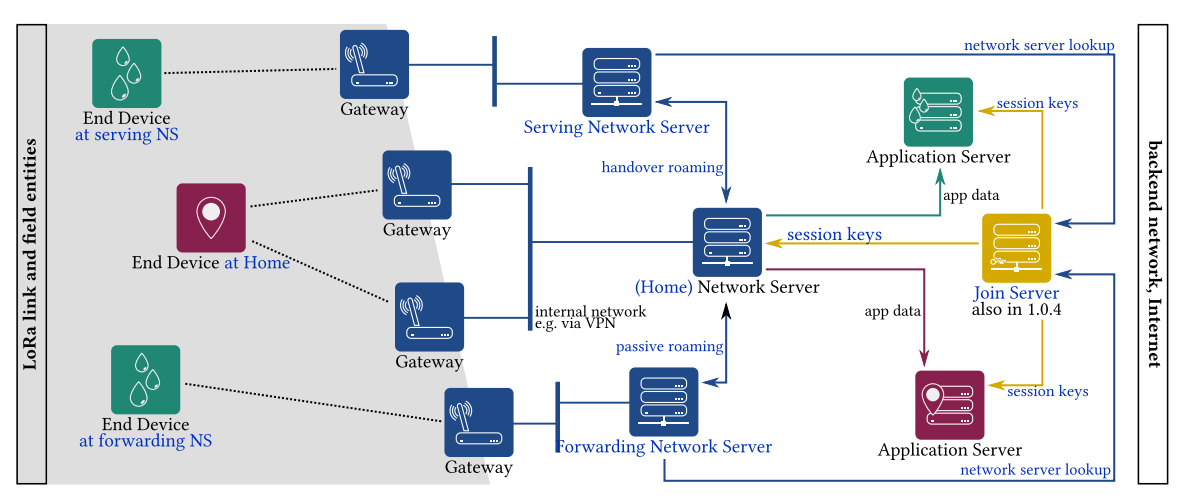
\includegraphics[scale=0.4]{barea/figuras/architeture_LoRaWan.png}
  \end{center}
  \legend{Fonte: \cite{hessel2023lorawan}}
\end{figure}

Após o encaminhamento feito pelos gateways, as mensagens chegam ao \textit{Network Server}. Esse servidor exerce papel central na rede, pois é responsável por processar as mensagens recebidas, eliminar duplicidades causadas pela recepção do mesmo quadro por múltiplos gateways, validar a integridade das mensagens e executar as funções de gerenciamento da camada MAC. Em outras palavras, é o \textit{Network Server} que coordena o funcionamento lógico da rede LoRaWAN.

Os dados de aplicação seguem então para o \textit{Application Server}, que é o componente responsável por tratar a informação útil transportada pelo dispositivo final. É nesse servidor que os dados recebidos podem ser decifrados, interpretados e encaminhados para a aplicação de interesse, como um sistema de monitoramento, um banco de dados ou uma plataforma de análise. Essa separação entre funções de rede e funções de aplicação é importante porque organiza melhor as responsabilidades do sistema e reduz o acoplamento entre comunicação e processamento da informação.

Na evolução do protocolo, especialmente a partir do LoRaWAN 1.1, o \textit{Join Server} passa a ter um papel mais explícito na arquitetura. Esse componente participa do processo de ativação dos dispositivos e da derivação de chaves de sessão, contribuindo para uma separação mais clara entre gerenciamento de rede e segurança da aplicação. Com isso, a arquitetura do LoRaWAN se torna mais organizada do ponto de vista funcional e mais adequada a cenários em que diferentes operadores ou domínios de serviço precisam cooperar.

Assim, a arquitetura do LoRaWAN pode ser entendida como uma organização em camadas funcionais: o dispositivo final coleta e transmite os dados, o gateway encaminha os quadros recebidos, o \textit{Network Server} gerencia a comunicação da rede, e o \textit{Application Server} entrega os dados à aplicação. Nas versões mais recentes, o \textit{Join Server} complementa essa estrutura ao apoiar o processo de ativação e gerenciamento de chaves. Essa divisão de papéis é fundamental para compreender como o protocolo opera e como seus componentes podem ser relacionados à arquitetura proposta neste trabalho.

%%%%%%%%%%%%%%%%%%%%%%%%%%%%%%%%%%%%%%%%%%%%%%%%%%%%

\subsection{Ativação do Dispositivo}

Antes de transmitir dados de aplicação, um dispositivo LoRaWAN precisa ser ativado na rede. Esse processo define como o dispositivo passa a ser reconhecido pelo sistema e como obtém o contexto necessário para a comunicação, incluindo identificadores, parâmetros de sessão e chaves utilizadas ao longo da operação. De forma geral, o LoRaWAN admite dois modos principais de ativação: \textit{Activation By Personalization} (ABP) e \textit{Over-The-Air Activation} (OTAA). \cite{hessel2023lorawan}

No modo ABP, o dispositivo já é configurado previamente com os parâmetros de sessão necessários para operar. Assim, ele pode iniciar a transmissão diretamente, sem realizar um procedimento de ingresso na rede a cada inicialização. Essa abordagem é mais simples do ponto de vista de implementação, mas oferece menor flexibilidade operacional, já que os parâmetros de comunicação ficam previamente fixados no dispositivo.

No modo OTAA, por outro lado, o dispositivo realiza um procedimento de ingresso na rede antes de iniciar sua operação normal. Nesse processo, o nó envia uma solicitação de ativação e, a partir da resposta da infraestrutura da rede, passa a operar com parâmetros e chaves de sessão derivados especificamente para aquela conexão. Em comparação com o ABP, essa abordagem é mais flexível e mais adequada a cenários reais, pois facilita renovação de chaves, adaptação do contexto de comunicação e suporte a funcionalidades mais avançadas do protocolo.

De forma simplificada, a ativação por OTAA envolve a troca de mensagens de ingresso e a geração de chaves de sessão a partir de credenciais previamente associadas ao dispositivo. Esse mecanismo permite que a rede estabeleça uma nova sessão de comunicação de forma controlada, em vez de depender sempre de parâmetros estáticos. Por esse motivo, o OTAA tende a ser considerado a alternativa mais robusta para implantações práticas, especialmente quando se deseja maior controle do ciclo de vida dos dispositivos e melhor suporte a segurança.

\begin{figure}[htb]
  \caption{\label{lorawan_join_process} (a) OTAA processo de entrada LoRaWAN 1.0.x. (b) OTAA processo de entrada LoRaWAN 1.1}
  \begin{center}
      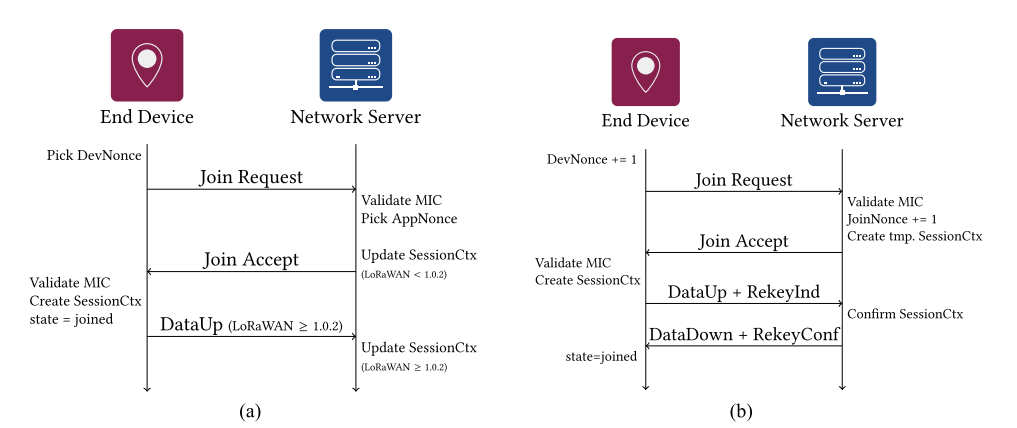
\includegraphics[scale=0.4]{barea/figuras/otaa_join_process.png}
  \end{center}
  \legend{Fonte: \cite{hessel2023lorawan}}
\end{figure}

A evolução do protocolo também impacta esse processo. Nas versões da família 1.0.x, a ativação já podia ocorrer por ABP ou OTAA, mas a versão 1.1 introduziu uma separação mais clara entre funções de rede e aplicação, além de mudanças no tratamento das chaves e no papel do \textit{Join Server}. Com isso, o processo de ativação passou a ser mais estruturado e alinhado com uma arquitetura de segurança mais organizada.

Assim, a ativação do dispositivo representa uma etapa fundamental no funcionamento do LoRaWAN, pois estabelece as condições iniciais para que a comunicação ocorra de forma válida dentro da rede. Enquanto o ABP oferece uma alternativa mais simples, o OTAA apresenta maior flexibilidade e melhor aderência a cenários práticos e escaláveis. A partir dessa etapa, o dispositivo pode iniciar a troca de dados com a infraestrutura da rede, conforme discutido na próxima subseção.

%%%%%%%%%%%%%%%%%%%%%%%%%%%%%%%%%%%%%%%%%%%%%%%%%%%%

\subsection{Transferência de Dados}

Após a ativação do dispositivo, a comunicação de dados pode ocorrer entre o dispositivo final e a infraestrutura da rede. No LoRaWAN, as mensagens enviadas pelo dispositivo em direção à rede são chamadas de \textit{DataUp}, enquanto as mensagens enviadas pela rede ao dispositivo são chamadas de \textit{Datadown}. Essa troca de dados pode ocorrer de forma simples, apenas com envio da informação, ou com solicitação de confirmação de recebimento, dependendo da necessidade da aplicação. \cite{hessel2023lorawan}

Quando não há necessidade de confirmação, utilizam-se mensagens não confirmadas, que reduzem o overhead da comunicação e tendem a ser mais adequadas a aplicações periódicas de monitoramento. Já nas mensagens confirmadas, a camada MAC pode exigir uma resposta da rede, permitindo ao dispositivo verificar se a transmissão foi reconhecida. Essa distinção é importante porque envolve um compromisso entre confiabilidade e consumo de recursos, já que confirmações adicionais aumentam o uso do canal e o gasto energético.

\begin{figure}[htb]
  \caption{\label{lorawan_message_ed}Classe para comunicacoes ED}
  \begin{center}
      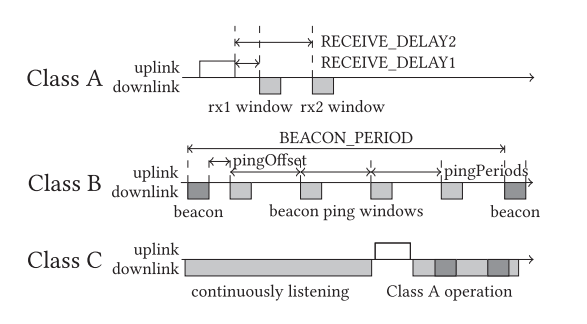
\includegraphics[scale=0.6]{barea/figuras/ed_operations_class.png}
  \end{center}
  \legend{Fonte: \cite{hessel2023lorawan}}
\end{figure}

O LoRaWAN define três modos principais de operação para os dispositivos finais, chamados de classes A, B e C. A Classe A é a padrão e está presente em todos os dispositivos LoRaWAN. Nela, o dispositivo inicia a comunicação por meio de um \textit{uplink} e, após essa transmissão, abre duas pequenas janelas de recepção para possíveis mensagens de \textit{downlink}. Essas janelas são conhecidas como RX1 e RX2. Esse modelo é o mais eficiente em termos energéticos, pois o dispositivo permanece a maior parte do tempo fora de escuta. 

Na Classe B, além do comportamento básico da Classe A, o dispositivo sincroniza sua operação com sinais periódicos da rede e passa a abrir janelas adicionais de recepção em instantes programados. Isso permite maior previsibilidade para o envio de mensagens em \textit{downlink}, embora aumente a complexidade da operação. Já na Classe C, o dispositivo permanece praticamente em escuta contínua, fechando a recepção apenas quando transmite. Essa abordagem reduz a latência de \textit{downlink}, mas aumenta significativamente o consumo de energia, sendo mais adequada a dispositivos com menor restrição energética.

\begin{figure}[htb]
  \caption{\label{messages_abc} Estrutura e Criptografia das mensagems LoRaWan}
    \begin{center}
      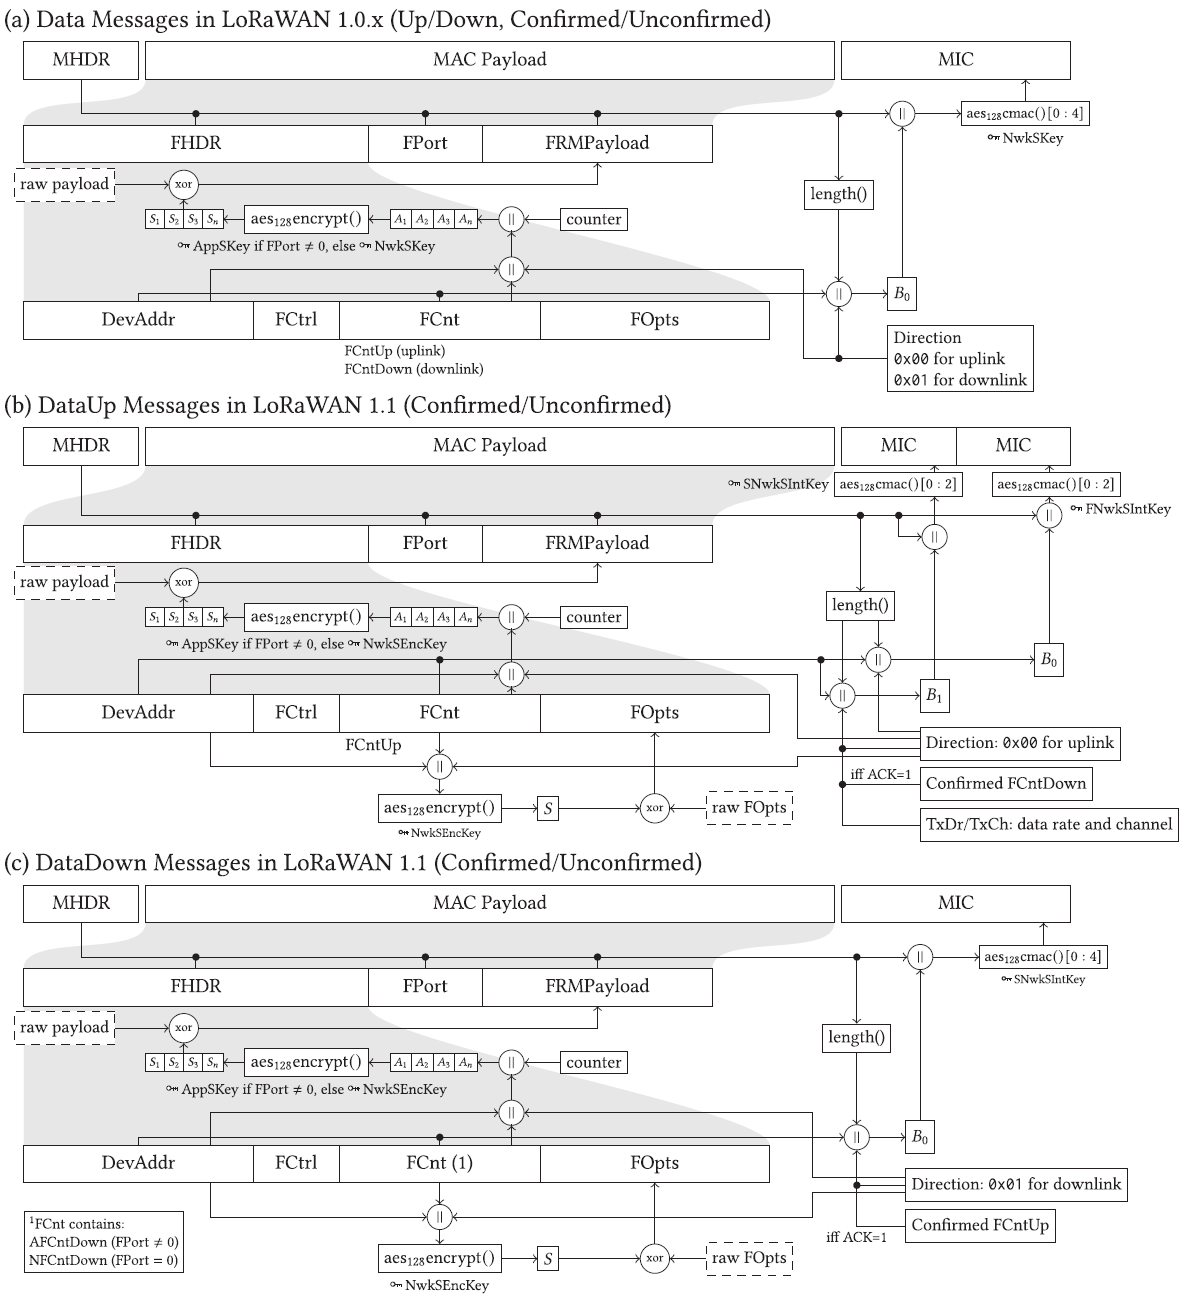
\includegraphics[scale=0.3]{barea/figuras/structure_messages_abc.png}
  \end{center}
  \legend{Fonte: \cite{hessel2023lorawan}}
\end{figure}

As mensagens de dados do LoRaWAN possuem uma estrutura padronizada. De forma geral, elas incluem um cabeçalho com a identificação do tipo de mensagem, um cabeçalho de quadro com informações de controle e endereçamento, um contador de quadros e o campo destinado à carga útil da aplicação. Entre esses elementos, o contador de quadros, representado por \textit{FCnt}, é especialmente importante para o acompanhamento da sequência das mensagens. Outros campos, como \textit{FPort} e \textit{FOpts}, ajudam a distinguir dados de aplicação e informações de controle da rede. Além disso, as mensagens incluem um código de integridade, chamado \textit{MIC}, utilizado para verificação da validade da comunicação.

De modo geral, a transferência de dados no LoRaWAN foi projetada para equilibrar simplicidade, baixo consumo e capacidade de operação em redes distribuídas de longo alcance. A existência de diferentes classes de operação e de mecanismos para mensagens confirmadas ou não confirmadas permite adaptar o comportamento da comunicação às necessidades da aplicação. A partir dessa base, torna-se possível compreender melhor como a rede ajusta e gerencia sua operação, tema discutido na próxima subseção.

%%%%%%%%%%%%%%%%%%%%%%%%%%%%%%%%%%%%%%%%%%%%%%%%%%%%

\subsection{Gerenciamento da Rede}

Como o LoRaWAN é um protocolo de camada MAC voltado a redes LPWAN, ele precisa de mecanismos para configurar dispositivos, ajustar parâmetros de comunicação e acompanhar o estado da rede. Parte dessas funções já aparece diretamente nos próprios campos das mensagens, como endereços, contadores de quadros e confirmações. No entanto, o protocolo também define comandos específicos para gerenciamento, conhecidos como \textit{MAC commands}, que permitem trocar informações de controle entre o dispositivo final e a infraestrutura da rede. \cite{hessel2023lorawan}

Esses comandos são usados para diferentes finalidades de operação. Entre elas, estão a obtenção de informações sobre a qualidade da conexão, o ajuste de parâmetros de transmissão e a sincronização de tempo. Assim, o gerenciamento da rede não ocorre como uma função separada do restante do protocolo, mas sim como parte do próprio fluxo de comunicação entre os dispositivos e os servidores da rede. 

Entre os mecanismos de gerenciamento, um dos mais importantes é o \textit{Adaptive Data Rate} (ADR). O ADR tem como objetivo ajustar a taxa de transmissão de dados e outros parâmetros de rádio de acordo com as condições de comunicação observadas na rede. Na prática, isso permite definir combinações mais adequadas de \textit{Spreading Factor}, largura de banda e potência de transmissão, buscando equilibrar confiabilidade, consumo de energia e uso eficiente do meio de comunicação.

De forma geral, o gerenciamento da rede no LoRaWAN existe para manter a comunicação funcional e eficiente ao longo do tempo. Por meio de comandos de controle e mecanismos como o ADR, o protocolo consegue ajustar seu comportamento às condições reais de operação, o que é especialmente importante em ambientes distribuídos, sujeitos a variações de alcance, interferência e disponibilidade energética. Com essa base conceitual, torna-se possível avançar para uma análise mais voltada à forma como essas tecnologias serão utilizadas na arquitetura proposta neste trabalho.

%%%%%%%%%%%%%%%%%%%%%%%%%%%%%%%%%%%%%%%%%%%%%%%%%%%%

\subsection{LoRa versus Wi-Fi no contexto do projeto}

Embora LoRa e Wi-Fi sejam tecnologias de comunicação sem fio, elas atendem a necessidades diferentes e, neste trabalho, não são tratadas como soluções concorrentes. Cada uma delas ocupa um papel específico na arquitetura proposta, de acordo com suas características de alcance, consumo energético, taxa de transmissão e facilidade de integração com os demais componentes do sistema.

O LoRa foi projetado para aplicações de longo alcance e baixo consumo, sendo adequado a dispositivos embarcados que operam com recursos limitados e transmitem pequenas quantidades de dados de forma periódica ou eventual. Essas características o tornam compatível com o cenário deste projeto, no qual o nó sensor precisa operar de forma eficiente, com comunicação sem fio e possibilidade de instalação afastada do ponto central da rede.

O Wi-Fi, por outro lado, oferece maior taxa de transmissão e integração mais direta com redes IP e serviços de aplicação, como APIs e servidores de armazenamento. Em contrapartida, apresenta maior consumo energético e menor adequação a nós distribuídos que precisem operar por longos períodos com restrição de energia. Por esse motivo, o Wi-Fi não foi adotado como tecnologia principal de comunicação entre os nós embarcados e a infraestrutura de campo.

No contexto deste trabalho, a solução adotada combina as duas tecnologias de forma complementar. O trecho entre o nó sensor e o \textit{gateway} utiliza LoRa em enlace ponto a ponto, preservando as vantagens de alcance e baixo consumo no nível embarcado. Já o trecho entre o \textit{gateway} e o servidor utiliza Wi-Fi, aproveitando sua integração mais simples com a infraestrutura de rede e com os serviços responsáveis por receber, armazenar e processar os dados coletados.

Essa divisão permite separar dois problemas distintos dentro da arquitetura. O primeiro é a comunicação entre dispositivos embarcados em campo, em que baixo consumo e cobertura são requisitos centrais. O segundo é a entrega dos dados para uma camada de processamento e persistência, em que a prioridade passa a ser conectividade com a rede local ou com a Internet, além da facilidade de integração com a aplicação. Assim, a escolha conjunta de LoRa e Wi-Fi não representa uma sobreposição de tecnologias, mas sim uma composição coerente entre camadas com funções diferentes.

Dessa forma, o uso de LoRa no trecho embarcado e de Wi-Fi no trecho de retaguarda estabelece uma arquitetura compatível com os objetivos do projeto. Ao mesmo tempo em que preserva as vantagens de uma rede LPWAN na comunicação entre os dispositivos de campo, essa abordagem também facilita a construção da interface com o servidor, a persistência dos dados e a futura integração com mecanismos de análise e segurança.

%%%%%%%%%%%%%%%%%%%%%%%%%%%%%%%%%%%%%%%%%%%%%%%%%%%%

\subsection{Implicações para a arquitetura proposta}
\label{subsec:implicacoes_arquitetura}

Os conceitos apresentados nas subseções anteriores permitem situar a arquitetura adotada neste trabalho. No projeto proposto, o nó sensor opera como dispositivo final, responsável pela coleta de dados do ambiente e pela transmissão dessas informações pela rede sem fio. Essa comunicação ocorre por um enlace LoRa ponto a ponto entre o nó e o \textit{gateway}, explorando as características de longo alcance e baixo consumo da camada física.

O gateway exerce o papel de ponto de transição entre a rede de campo e a infraestrutura de retaguarda. Sua função principal é receber os quadros enviados pelos dispositivos finais e encaminhá-los para a camada de processamento do sistema. A partir desse ponto, os dados podem ser entregues a um servidor ou API responsável por armazenamento, organização e disponibilização das informações para etapas posteriores de análise.

Essa divisão é importante porque separa o problema da comunicação embarcada do problema de processamento dos dados. No nível dos nós em campo, o foco está em transmitir com eficiência, respeitando restrições de energia, alcance e capacidade computacional. Já no nível do gateway e do servidor, torna-se possível concentrar funções de persistência, observabilidade e integração com serviços de aplicação, sem impor esse custo diretamente aos dispositivos finais.

A opção pelo enlace ponto a ponto, em lugar de uma rede LoRaWAN completa, é uma decisão de projeto, e não apenas uma consequência do hardware disponível. Uma rede LoRaWAN exige \textit{gateway} multicanal e \textit{network server}, e sua camada MAC determina o uso de AES-128 para proteger todo quadro. Nesse contexto, a inserção de outra primitiva criptográfica seria redundante, e a comparação entre algoritmos perderia sentido. O enlace ponto a ponto, ao contrário, deixa a camada acima da física inteiramente sob controle da aplicação, o que abre o espaço de projeto no qual a escolha do algoritmo de criptografia autenticada pode ser feita e avaliada. Além disso, controlar as duas pontas do enlace permite conhecer o instante e o conteúdo de cada transmissão, condição necessária para rotular o que é operação normal e o que é anomalia.

O LoRaWAN permanece como modelo de referência. Os papéis de \textit{gateway}, \textit{network server} e \textit{application server}, separados na arquitetura da Figura~\ref{lorawan_architeture}, são aqui concentrados em um único dispositivo, o \textit{gateway}, que recebe, valida e encaminha os quadros. A estrutura do quadro transmitido segue a do PHYPayload da especificação 1.0.4: o identificador do dispositivo e o contador de quadros vão em claro, e a alteração de qualquer um dos dois invalida o código de autenticação que encerra o quadro, depois do \textit{payload} cifrado. O esquema de provisionamento equivale à ativação por personalização (ABP), com chave e identificador gravados no dispositivo e sem procedimento de ingresso. O formato do quadro e a ordem de validação implementados são descritos na Subseção~\ref{subsec:implementacao_infra}.

Como discutido na Subseção~\ref{subsec:camada_fisica_lora}, a camada física LoRa não oferece nenhum mecanismo de segurança, e em um enlace ponto a ponto não existe a camada MAC do LoRaWAN que os forneceria. A proteção do quadro contra leitura, modificação, forja e repetição precisa, portanto, ser fornecida pela própria aplicação. Ao mesmo tempo, a presença de dados trafegando entre o dispositivo embarcado, o \textit{gateway} e a infraestrutura de \textit{backend} exige que a proteção seja pensada para cada trecho, e não apenas para o enlace de rádio.

Além disso, a própria dinâmica operacional da rede produz informações que podem ser úteis para análise de comportamento, identificação de falhas e detecção de atividades anômalas. Parâmetros de transmissão, padrões temporais de envio e eventos observados na comunicação podem servir como base para uma camada adicional de monitoramento do sistema, complementando a proteção oferecida pelos mecanismos tradicionais do protocolo.

Dessa forma, a arquitetura proposta neste trabalho não se limita ao transporte de dados entre dispositivos e servidor. Ela também cria as condições para incorporar camadas complementares de segurança e análise. Nesse contexto, a próxima seção discute o uso de criptografia leve como mecanismo adequado à proteção de dados em dispositivos com recursos restritos, enquanto a seção seguinte apresenta o papel do \textit{Machine Learning} como apoio à análise do comportamento da rede e à detecção de anomalias.


%%%%%%%%%%%%%%%%%%%%%%%%%%%%%%%%%%%%%%%%%%%%%%%%%%%%
%%%%%%%%%%%%%%%%%%%%%%%%%%%%%%%%%%%%%%%%%%%%%%%%%%%%


\section{Criptografia Leve (Lightweight Cryptography) e o Padrão Ascon}
Em dispositivos IoT, onde o baixo consumo de energia é um requisito essencial para viabilizar operações em diversas áreas, as aplicações que lidam com dados sensíveis e exigem sigilo demandam a adoção de métodos criptográficos que sejam, simultaneamente, leves e seguros.

O Instituto Nacional de Padrões e Tecnologia dos Estados Unidos (NIST) atua, desde 1973, no desenvolvimento de normas para proteger dados sensíveis transmitidos entre dispositivos. Seu histórico abrange desde a criação do \textit{Data Encryption Standard} (DES) e a consolidação do atual padrão de criptografia simétrica, o \textit{Advanced Encryption Standard} (AES), até as recentes padronizações de criptografia pós-quântica (\textit{Post-Quantum Cryptography}) e de criptografia leve (\textit{Lightweight Cryptography}) \cite{chen2022cornerstone}.

Com o crescimento expressivo do uso de dispositivos IoT, a necessidade de estabelecer um padrão robusto de criptografia leve tornou-se urgente. Isso impulsionou o desenvolvimento de uma nova padronização internacional com o objetivo de contemplar as primitivas criptográficas e os modos de operação adequados para ambientes restritos. Os critérios exigidos para esse novo padrão incluíam resiliência de segurança, flexibilidade de implementação, baixa sobrecarga ao integrar múltiplas funções e facilidade de proteção contra ataques de canal lateral (\textit{Side-Channel Attacks}), entre outros requisitos técnicos \cite{nistir8114}.

O processo de padronização promovido pelo NIST ocorreu ao longo de múltiplas fases de testes e escrutínio público. Inicialmente, 57 algoritmos foram submetidos para consideração. Desses, 32 avançaram para a segunda rodada e, após rigorosas avaliações de desempenho e segurança, apenas 10 chegaram à fase final. A culminação desse extenso projeto ocorreu, em 2023, com o anúncio da família Ascon como a grande vencedora \cite{nistir8454}.

O desenvolvimento do padrão Ascon começou em 2014 e ele é o foco principal deste trabalho. Na prática, ele funciona como um conjunto de algoritmos construído sob medida para dispositivos com poucos recursos. A padronização oficial conta com quatro variações principais. A primeira delas é o Ascon-AEAD128, de criptografia autenticada com dados associados (AEAD, \textit{Authenticated Encryption with Associated Data}), que criptografa os dados, verifica a autenticidade da mensagem e facilita a proteção contra ataques de canal lateral. A segunda variação é o Ascon-Hash256, criado especificamente para garantir a integridade dos dados transmitidos pela rede. Por fim, existem o Ascon-XOF128 e o Ascon-CXOF128. Ambos funcionam como funções de saída extensível, uma característica que permite ajustar o tamanho do \textit{hash} gerado e economizar recursos computacionais durante o processamento \cite{nist2025ascon}.

%%%%%%%%%%%%%%%%%%%%%%%%%%%%%%%%%%%%%%%%%%%%%%%%%%%%

\subsection{O Padrão Ascon-AEAD128 e a Variante Ascon-128a}
O algoritmo de criptografia autenticada escolhido para o projeto pertence à família Ascon, padronizada pelo NIST sob a forma do Ascon-AEAD128 \cite{nist2025ascon}. Na prática, a implementação adotada neste trabalho utiliza a variante Ascon-128a, finalista do processo de padronização (versão 1.2), que compartilha a mesma estrutura de permutação do algoritmo padronizado, conforme detalhado na Seção \ref{subsec:biblioteca-ascon}. A utilização de funções de \textit{hash} adicionais não é necessária, uma vez que esse algoritmo já garante confidencialidade, integridade e autenticidade em uma única operação de criptografia autenticada.

O processo de cifragem do Ascon-AEAD128 (Figura~\ref{fig:fluxo_ascon_encript}) recebe como entrada uma chave secreta e um \textit{nonce}, ambos de 128 bits, além dos dados associados (\textit{Associated Data} - AD) e o texto em claro a ser cifrado (\textit{plaintext}), que possuem tamanhos variáveis. A saída dessa função é o texto cifrado (\textit{ciphertext}) acompanhado de uma \textit{Tag} de Autenticação de 128 bits. Por sua vez, a função de decifragem recebe a chave, o \textit{nonce}, os dados associados, o texto cifrado e a \textit{tag} de autenticação. O texto original em claro só é retornado se a \textit{tag} for validada com sucesso. Caso contrário, a operação é abortada e retorna um erro (\textit{fail}).

O estado interno inicial de ambos os processos possui 320 bits, sendo formado pela concatenação de 64 bits do Vetor de Inicialização (IV), 128 bits da chave secreta e 128 bits do \textit{nonce}. Após a inicialização, o algoritmo segue em fases. Primeiro ocorre o processamento dos dados associados (se presentes), seguido pela cifragem do texto em blocos e, ao final de todo o processamento, a fase de finalização gera a \textit{tag} de autenticação.

A Tabela~\ref{tab:parametros_ascon} compara os parâmetros do Ascon-AEAD128 padronizado com os da variante Ascon-128a adotada neste trabalho. Todos os valores que determinam o custo de processamento, como a taxa, a capacidade e o número de rodadas das permutações, são idênticos nas duas versões, o que sustenta a equivalência de desempenho assumida na Seção \ref{subsec:biblioteca-ascon}.

\begin{table}[htb]
\centering
\caption{Parâmetros do Ascon-AEAD128 padronizado e da variante Ascon-128a}
\label{tab:parametros_ascon}
\begin{tabular}{lrr}
\hline
\textbf{Parâmetro} & \textbf{Ascon-AEAD128} & \textbf{Ascon-128a} \\
\hline
Chave (bits) & 128 & 128 \\
\textit{Nonce} (bits) & 128 & 128 \\
\textit{Tag} de autenticação (bits) & 128 & 128 \\
Taxa de absorção (bits) & 128 & 128 \\
Capacidade (bits) & 192 & 192 \\
Rodadas na inicialização e finalização & 12 & 12 \\
Rodadas no processamento de dados & 8 & 8 \\
\hline
\end{tabular}
\legend{Fonte: elaborado pelos autores com base em \citeonline{nist800232} e \citeonline{ascon_v12_spec}.}
\end{table}

\begin{figure}[htb]
  \caption{\label{fig:fluxo_ascon_encript}Processo de cifragem do Ascon-AEAD128}
  \begin{center}
    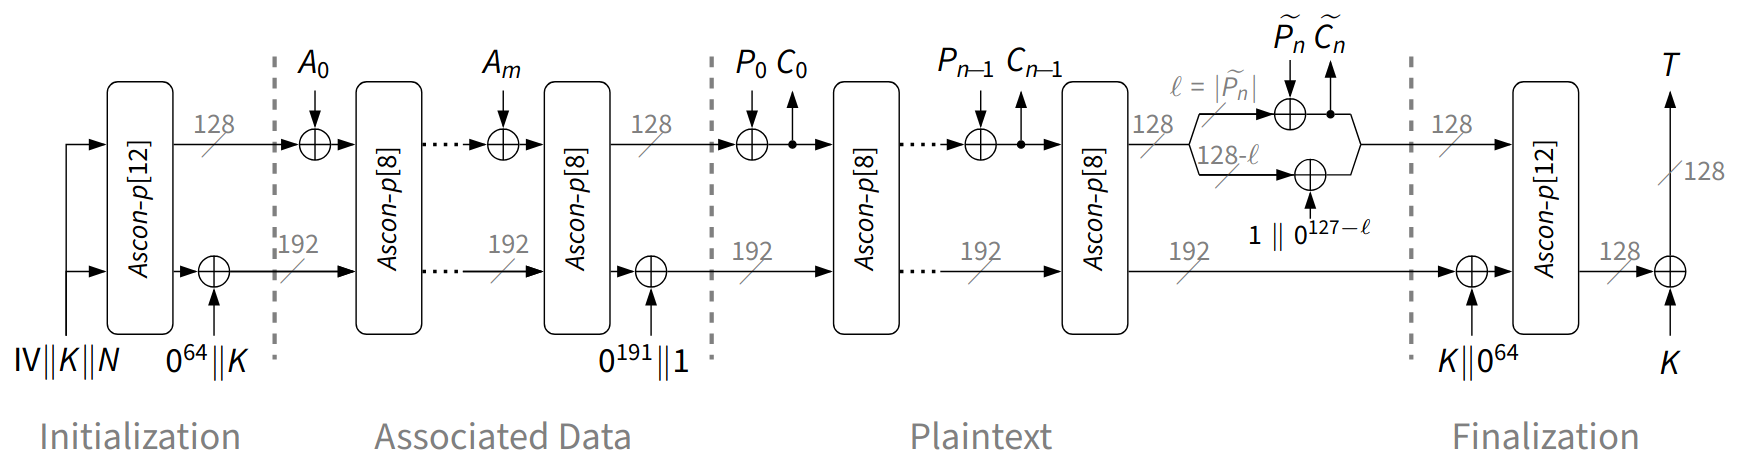
\includegraphics[scale=0.25]{felipe/figuras/fluxo-ascon-aead128-encript.png}
  \end{center}
  \legend{Fonte: \cite{nist2025ascon}}
\end{figure}

O processo de decifragem (Figura~\ref{fig:fluxo_ascon_decript}) possui uma estrutura muito semelhante à da cifragem. Ele passa pela mesma inicialização do estado de 320 bits e pelo processamento dos dados associados. A diferença principal ocorre nas etapas finais. O texto cifrado é processado bloco a bloco para recuperar o texto original e, na fase de finalização, a chave secreta é combinada com o estado interno para recalcular a \textit{tag} de autenticação. Se a \textit{tag} recalculada for idêntica à \textit{tag} recebida, o texto decifrado é considerado autêntico e é retornado, caso contrário, a mensagem é descartada.

\begin{figure}[htb]
  \caption{\label{fig:fluxo_ascon_decript}Processo de decifragem do Ascon-AEAD128}
  \begin{center}
    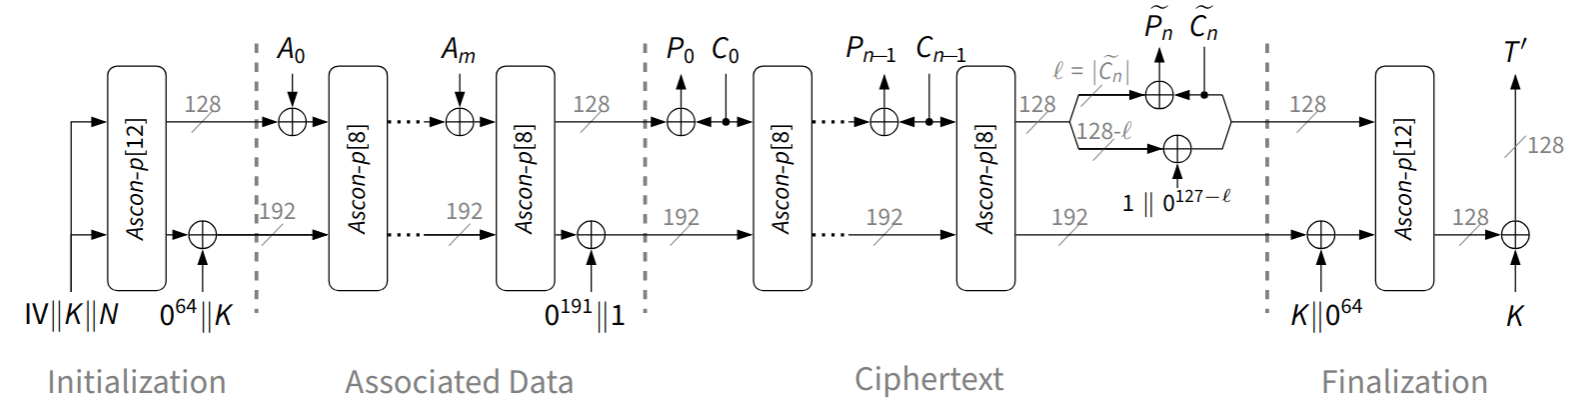
\includegraphics[scale=0.35]{felipe/figuras/fluxo-ascon-aead128-decript.png}
  \end{center}
  \legend{Fonte: \cite{nist2025ascon}}
\end{figure}

%%%%%%%%%%%%%%%%%%%%%%%%%%%%%%%%%%%%%%%%%%%%%%%%%%%%

\subsection{Comparativo de Algoritmos Criptográficos para IoT}
Durante a pesquisa inicial sobre criptografia leve, outros algoritmos foram avaliados, mas nenhum se mostrou tão adequado às necessidades do projeto quanto o padrão Ascon. Entre as principais alternativas analisadas, destacam-se o Speck \cite{beaulieu2013speck} e o ChaCha20 \cite{bernstein2008chacha}.

O Speck é uma cifra de bloco pura e bastante leve. No entanto, ele possui uma limitação estrutural importante para redes modernas, pois não oferece Criptografia Autenticada com Dados Associados (\textit{AEAD}) de forma nativa. Para garantir a integridade da mensagem, seria necessária a adição de um algoritmo de autenticação secundário e independente (como um código de autenticação de mensagem, MAC). O Speck teve sua padronização internacional ativamente rejeitada pela ISO (\textit{International Organization for Standardization}) por falta de transparência em seu design \cite{register2018nsa}.

O ChaCha20, por sua vez, é uma cifra de fluxo de altíssimo desempenho, amplamente adotada como padrão da indústria para cenários de \textit{software} onde \textbf{não} há aceleração de \textit{hardware} disponível. Contudo, assim como o Speck, ele carece de propriedades \textit{AEAD} embutidas. A exigência extra de se acoplar o algoritmo Poly1305 consome memória e processamento. Assim, ele não atende ao requisito de reunir confidencialidade, integridade e autenticidade em uma única operação, oferecido nativamente pelo Ascon.

Para a análise comparativa de viabilidade, este trabalho também optou por não focar nos demais algoritmos finalistas do processo de padronização do NIST (como TinyJAMBU ou Xoodyak) \cite{nist_lwc_finalists}, uma vez que o próprio comitê apontou o Ascon como o mais maduro dos finalistas em termos de segurança e como a submissão com maior volume de análise independente, no relatório oficial NIST IR 8454 \cite{nistir8454}.

Dessa forma, a metodologia de comparação deste trabalho foi refinada para responder à questão prática sobre o embate entre o novo padrão de \textit{software} e o padrão legado de \textit{hardware}. Os testes comparam exclusivamente o Ascon (novo padrão \textit{Lightweight Cryptography} do NIST) contra o AES-128-GCM (\textit{Galois/Counter Mode}), cujo bloco de cifra é executado no coprocessador de \textit{hardware} do microcontrolador, enquanto a autenticação (GHASH) permanece em \textit{software}. Essa abordagem permite avaliar se a migração para a criptografia leve em \textit{software} traz vantagens reais de consumo, memória e latência frente ao uso do acelerador de silício já embutido nas placas comerciais utilizadas em redes \textit{LoRaWAN}.

%%%%%%%%%%%%%%%%%%%%%%%%%%%%%%%%%%%%%%%%%%%%%%%%%%%%
%%%%%%%%%%%%%%%%%%%%%%%%%%%%%%%%%%%%%%%%%%%%%%%%%%%%


\section{Aprendizado de Máquina para Detecção de Anomalias}
\label{sec:ml-conceitos}

O uso de aprendizado de máquina é coerente com o estado da arte recente.
Trabalhos como \cite{farhad2023} demonstram que o aprendizado de máquina em
LoRaWAN vem sendo explorado para otimizar parâmetros de rede
(\textit{spreading factor}, potência de transmissão) e classificar padrões
de mobilidade. Embora parte significativa da literatura esteja concentrada em
desempenho e eficiência, esse mesmo conjunto de atributos também é relevante
para a detecção de anomalias, já que comportamentos suspeitos se refletem em
mudanças desses padrões operacionais \cite{farhad2023, vangelista2023}.

Esta seção trata dos conceitos de séries temporais e de detecção de anomalias
usados pela frente de aprendizado de máquina. Eles sustentam o método da
Seção~\ref{subsec:ml-dataset} e os resultados da Seção~\ref{sec:resultados_ml}.

%%%%%%%%%%%%%%%%%%%%%%%%%%%%%%%%%%%%%%%%%%%%%%%%%%%%

\subsection{Por que detectar desvios do RSSI}
\label{subsec:ml-motivacao}

A autenticação de um quadro, pelo código de integridade do LoRaWAN ou pela
\textit{tag} do Ascon usada no protótipo da equipe, mostra que o remetente
conhece a chave da sessão. Ela não mostra de onde o sinal partiu. Se a chave de
um nó sensor for obtida por um atacante, os quadros que ele enviar serão
aceitos como legítimos, e o conteúdo não permite distingui-los dos do nó
verdadeiro. Esse é o caso de \textit{spoofing} que a criptografia não cobre.

O que ainda diferencia o atacante é a camada física. Um transmissor em outra
posição, ou com outra potência, chega ao \textit{gateway} com outro RSSI, e o
\textit{gateway} já mede o RSSI de todo quadro, sem mudança no protocolo. Na
literatura, desvios do RSSI fora da faixa esperada para o nó são tratados como
indício de \textit{spoofing} \cite{pourghasem2025spoofing}, e desvios nos
metadados de rádio, entre eles o RSSI, expõem o \textit{jamming} reativo
\cite{ruotsalainen2022jamming}.

O RSSI, porém, também muda sem ataque, com o canal de frequência, a taxa de
dados e o ambiente (Seção~\ref{subsec:ml-rssi}). Um desvio só tem significado
em relação ao valor esperado para aquele nó naquele momento. Por isso a
detecção deste trabalho prevê o RSSI de cada quadro e alarma quando o valor
observado se afasta da previsão além de um limiar
(Seção~\ref{subsec:ml-deteccao}). Prever, em vez de comparar com um valor
fixo, acompanha as mudanças de nível que acontecem sem ataque, e não exige
exemplos rotulados de ataque para o treino. Como a previsão usa só quadros
passados, a decisão pode ser tomada no próprio \textit{gateway}, quando cada
quadro chega \cite{blazquez2021review}, o que pede um modelo leve o bastante
para um microcontrolador.

\subsection{O RSSI como série temporal}
\label{subsec:ml-rssi}

O RSSI é a potência com que o \textit{gateway} recebe um quadro, em dBm. O
valor é negativo e é mais forte quanto mais perto de zero \cite{ttnrssi}. O nó
sensor não escolhe o \textit{gateway}. Todos os \textit{gateways} ao alcance
recebem o mesmo quadro, e cada um mede o seu próprio RSSI
\cite{brocaarintegration}. Para formar uma série temporal é preciso, portanto,
fixar um par de nó sensor e \textit{gateway}. Como o RSSI é medido no
\textit{gateway}, ele fica fora da proteção dada pela cifragem do
\textit{payload}.

O RSSI muda também sem ataque. O nó sensor troca de canal de frequência de
forma pseudoaleatória a cada transmissão \cite{lorawan103}, e a taxa de dados
adaptativa (ADR) pode mudar a taxa de dados e a potência de transmissão
\cite{ttnadr}. Além disso, um contador de quadros (FCnt) repetido indica o
mesmo quadro enviado de novo, e não uma medida nova \cite{lorawan103}.

\subsection{Autocorrelação e estacionariedade}
\label{subsec:ml-autocorrelacao}

A função de autocorrelação (ACF) mede a relação linear entre a série e ela
mesma deslocada de $k$ passos, chamados de defasagem. A função de
autocorrelação parcial (PACF) mede a mesma relação depois de remover o efeito
das defasagens intermediárias \cite{hyndman2021}.

Uma série é estacionária quando as suas propriedades estatísticas não dependem
do instante observado. A diferenciação, que troca cada valor pela diferença em
relação ao anterior, remove mudanças de nível. No teste KPSS, a hipótese nula é
que a série é estacionária, e um valor-p pequeno indica que é preciso
diferenciar \cite{hyndman2021}.

\subsection{Modelos de previsão}
\label{subsec:ml-modelos}

A referência mais simples é o \textit{random walk}, cuja previsão é a última
observação \cite{hyndman2021}, como na Equação~\ref{eq:ml-random-walk}.
\begin{equation}
	\hat{y}_t = y_{t-1}
	\label{eq:ml-random-walk}
\end{equation}

O ARIMA$(p,d,q)$ combina $p$ termos autorregressivos, $d$ diferenciações e $q$
termos de médias móveis dos erros anteriores \cite{box2015, hyndman2021}. Com o
operador de atraso $B$, tal que $B y_t = y_{t-1}$, o modelo se escreve como na
Equação~\ref{eq:ml-arima}, em que $\varepsilon_t$ é um ruído branco.
\begin{equation}
	\left(1 - \phi_1 B - \dots - \phi_p B^p\right)(1-B)^d y_t = c + \left(1 + \theta_1 B + \dots + \theta_q B^q\right)\varepsilon_t
	\label{eq:ml-arima}
\end{equation}

O \textit{random walk} é o caso ARIMA$(0,1,0)$, e o ARIMA$(0,1,1)$ equivale à
suavização exponencial simples \cite{hyndman2021}. Os coeficientes podem ser
estimados uma vez e depois aplicados, fixos, a uma série mais longa
\cite{statsmodelsapply}. Assim se obtém a previsão um passo à frente, em que
cada valor é previsto com as observações reais até o instante anterior.

\subsection{Avaliação da previsão}
\label{subsec:ml-avaliacao}

Os dados de treino estimam os parâmetros, e os de teste, que não entram no
ajuste, medem a acurácia. Em séries temporais a divisão é cronológica, para que
nenhuma informação futura entre no treino \cite{hyndman2021, bergmeir2012}.
Entre treino e teste, um conjunto de validação serve para as escolhas, como a
ordem do modelo, de modo que o teste seja usado só para a medida final.

O erro de previsão é medido por duas métricas na unidade dos dados, a raiz do
erro quadrático médio (RMSE) e o erro absoluto médio (MAE), definidas nas
Equações~\ref{eq:ml-rmse} e~\ref{eq:ml-mae} \cite{hyndman2021}.
\begin{equation}
	\mathrm{RMSE} = \sqrt{\frac{1}{N}\sum_{t=1}^{N}\left(y_t - \hat{y}_t\right)^2}
	\label{eq:ml-rmse}
\end{equation}
\begin{equation}
	\mathrm{MAE} = \frac{1}{N}\sum_{t=1}^{N}\left|y_t - \hat{y}_t\right|
	\label{eq:ml-mae}
\end{equation}
O RMSE dá mais peso aos erros grandes, e o MAE pesa todos os erros igualmente.
Um método que minimiza o MAE leva a previsões da mediana, e um que minimiza o
RMSE, a previsões da média \cite{hyndman2021}. Uma diferença de ordem entre as
duas métricas indica que a comparação depende do tamanho dos erros
considerados.

\subsection{Detecção de anomalias por previsão}
\label{subsec:ml-deteccao}

Em operação real, dados rotulados que identifiquem quadros associados a
ataques são raros, o que dificulta o uso de classificadores supervisionados.
Por isso a detecção é tratada como um problema de previsão. Um modelo estima o
valor esperado de cada observação a partir das anteriores, e o ponto é
declarado anômalo quando a distância entre o valor observado $x_t$ e o valor
esperado $\hat{x}_t$ passa de um limiar $\tau$ \cite{blazquez2021review,
chalapathy2019}, como na Equação~\ref{eq:ml-deteccao}. Quando $\hat{x}_t$ vem
só de observações passadas, a decisão é tomada sobre cada dado no momento em
que ele chega, o que permite executá-la na borda da rede.
\begin{equation}
	\left| x_t - \hat{x}_t \right| > \tau
	\label{eq:ml-deteccao}
\end{equation}

Sob resíduos normais e sem correlação, $\tau$ pode ser $c$ vezes o desvio
padrão dos resíduos, com $c = 2{,}58$ para 99\% \cite{hyndman2021}. Quando a
suposição de normalidade falha, um limiar não paramétrico, tirado da própria
distribuição dos erros, é uma alternativa \cite{hundman2018spacecraft}. Em
LoRaWAN, o \textit{jamming} reativo aumenta o RSSI e é detectado comparando os
metadados recebidos com os esperados para o nó sensor
\cite{ruotsalainen2022jamming}, e desvios do RSSI fora da faixa esperada são
tratados como indício de \textit{spoofing} \cite{pourghasem2025spoofing}.

\subsection{Trabalhos relacionados e lacuna}
\label{subsec:ml-lacuna}

A literatura sobre o RSSI em redes LoRaWAN se divide em duas linhas que pouco se
encontram. A primeira prevê o RSSI. \citeonline{guerra2024forecasting}
compararam ARIMA, inteligência artificial e modelos híbridos em médias horárias
de oito nós, e o ARIMA com a temperatura como variável externa foi a
alternativa mais competitiva. \citeonline{fhima2026harbors} previram vários
passos à frente o RSSI de nós móveis num porto, reajustando o modelo a cada
ponto. Nenhum dos dois usa a previsão para detectar anomalias, nem trata o
canal de frequência, que \citeonline{harinda2022multigateway} não viram afetar o
RSSI em ambiente interno.

A segunda linha detecta ataques pelos metadados de rádio.
\citeonline{ruotsalainen2022jamming} compara os metadados recebidos com os
esperados para o nó, e \citeonline{pourghasem2025spoofing} classificam quadros
com modelos supervisionados, o que exige rótulos de ataque. Falta, entre as duas
linhas, um modelo leve que forneça o valor esperado de cada quadro, com uma
sensibilidade medida em dB e um alarme falso controlado, e que rode no próprio
\textit{gateway}. Este trabalho ocupa essa lacuna com os metadados de rádio do
\textit{dataset} Tour Perret \cite{tourperret_dataset} e com a execução do
detector num microcontrolador ESP32.



% Capítulo 3. Metodologia do Trabalho
\chapter{Método do trabalho} \label{cap:metodo}


Este capítulo apresenta o método adotado na construção da proposta deste trabalho. A definição da solução foi conduzida a partir de três frentes complementares: levantamento bibliográfico, análise técnica das tecnologias envolvidas e organização da arquitetura do sistema. O objetivo desse processo foi estruturar uma proposta coerente para comunicação, segurança e análise de dados em um cenário de sistemas embarcados e Internet das Coisas.

Inicialmente, é apresentada a arquitetura de comunicação e infraestrutura do sistema, que estabelece o caminho de coleta, encaminhamento e armazenamento dos dados. Em seguida, são apresentadas as etapas relacionadas à segurança e ao uso de aprendizado de máquina, consideradas como partes integradas à solução proposta. Ao final, o capítulo organiza os elementos que orientam a implementação e a avaliação do sistema.

%%%%%%%%%%%%%%%%%%%%%%%%%%%%%%%%%%%%%%%%%%%%%%%%%%%%
%%%%%%%%%%%%%%%%%%%%%%%%%%%%%%%%%%%%%%%%%%%%%%%%%%%%

\section{Procedimento de definição da arquitetura do sistema}

A definição da arquitetura do sistema foi conduzida a partir da combinação entre levantamento bibliográfico, análise técnica das tecnologias envolvidas e separação em módulos da solução proposta. O objetivo dessa etapa foi estruturar uma arquitetura coerente com o problema estudado, considerando as restrições típicas de sistemas embarcados, a necessidade de comunicação em campo e a integração posterior com mecanismos de segurança e análise.

Como referência metodológica para essa definição, o trabalho adota princípios inspirados no modelo RM-ODP, utilizando diferentes pontos de vista para organizar a solução. Em termos funcionais, foram identificados os principais blocos responsáveis pela coleta, encaminhamento, recebimento e armazenamento das informações. Em termos de informação, foram considerados os dados de aplicação e os metadados necessários para rastreabilidade, segurança e análise posterior. Em termos de engenharia, foram observadas as separações entre o trecho embarcado da comunicação, o gateway e a infraestrutura de backend.

A partir dessa organização, a arquitetura foi estruturada de modo a separar claramente a comunicação em campo da camada de aplicação. Essa separação permite tratar, de forma independente, as restrições energéticas dos nós sensores, o papel intermediário do gateway e as funções de autenticação, persistência e análise associadas ao backend. Com isso, a definição arquitetural deixa de ser apenas uma escolha de componentes e passa a refletir a distribuição de responsabilidades entre as partes do sistema.

Além da decomposição dos componentes, o procedimento de definição da arquitetura também considerou o fluxo das informações ao longo da solução. Para isso, foram analisadas as interações entre os nós de campo, o gateway e a infraestrutura de backend, buscando garantir que o sistema fosse capaz de receber, registrar e armazenar dados e metadados de forma compatível com as etapas posteriores do trabalho.

Por fim, a representação da interação entre os principais componentes foi organizada também por meio de diagramas, de modo a tornar mais clara a sequência de eventos envolvida na coleta, no encaminhamento e no armazenamento das mensagens. Essa modelagem auxilia tanto na compreensão da proposta quanto na transição entre a etapa metodológica e a etapa posterior de especificação da arquitetura.

\subsection{Critérios adotados na decomposição arquitetural}

A modularização da arquitetura foi orientada por três critérios principais. O primeiro foi a separação entre o trecho de comunicação em campo e a infraestrutura de aplicação, de modo a preservar as vantagens do uso de LoRa no nível embarcado e da comunicação baseada em rede IP no nível de backend. O segundo foi a definição de responsabilidades distintas para coleta, encaminhamento, autenticação e persistência, evitando concentrar funções heterogêneas em um único componente. O terceiro foi a necessidade de manter a solução compatível com a incorporação posterior de mecanismos de criptografia leve e análise por aprendizado de máquina.

Esses critérios levaram à definição de uma arquitetura em blocos com papéis bem delimitados. No trecho embarcado, concentram-se as funções de aquisição e transmissão inicial dos dados. No ponto de transição, o gateway atua como elemento de integração entre a rede de campo e a infraestrutura de aplicação. No backend, concentram-se as funções de autenticação, persistência e preparação dos dados para uso posterior. Essa divisão favorece clareza arquitetural, reduz acoplamento entre responsabilidades e facilita a evolução incremental da solução.

\subsection{Modelagem das interações e do fluxo de dados}

Para explicitar a dinâmica de funcionamento da proposta, o fluxo principal de interação entre os componentes foi modelado em termos de sequência de eventos. Essa modelagem considera a coleta dos dados no nó de campo, a transmissão pelo enlace LoRa ponto a ponto, a recepção e o enriquecimento da mensagem no gateway, o encaminhamento ao backend por Wi-Fi e HTTP, e o armazenamento final de dados e metadados na infraestrutura de persistência.

A utilização de um diagrama de sequência nessa etapa é importante porque permite representar, de forma mais direta, a ordem das interações entre os componentes e os pontos em que ocorre o tratamento das mensagens. Com isso, o fluxo deixa de ser apenas uma descrição textual e passa a ser apresentado também como uma sequência organizada de ações entre entidades bem definidas.

\begin{figure}[htb]
  \caption{\label{infra_arch_1}Diagrama de sequência UML do fluxo principal}
  \begin{center}
      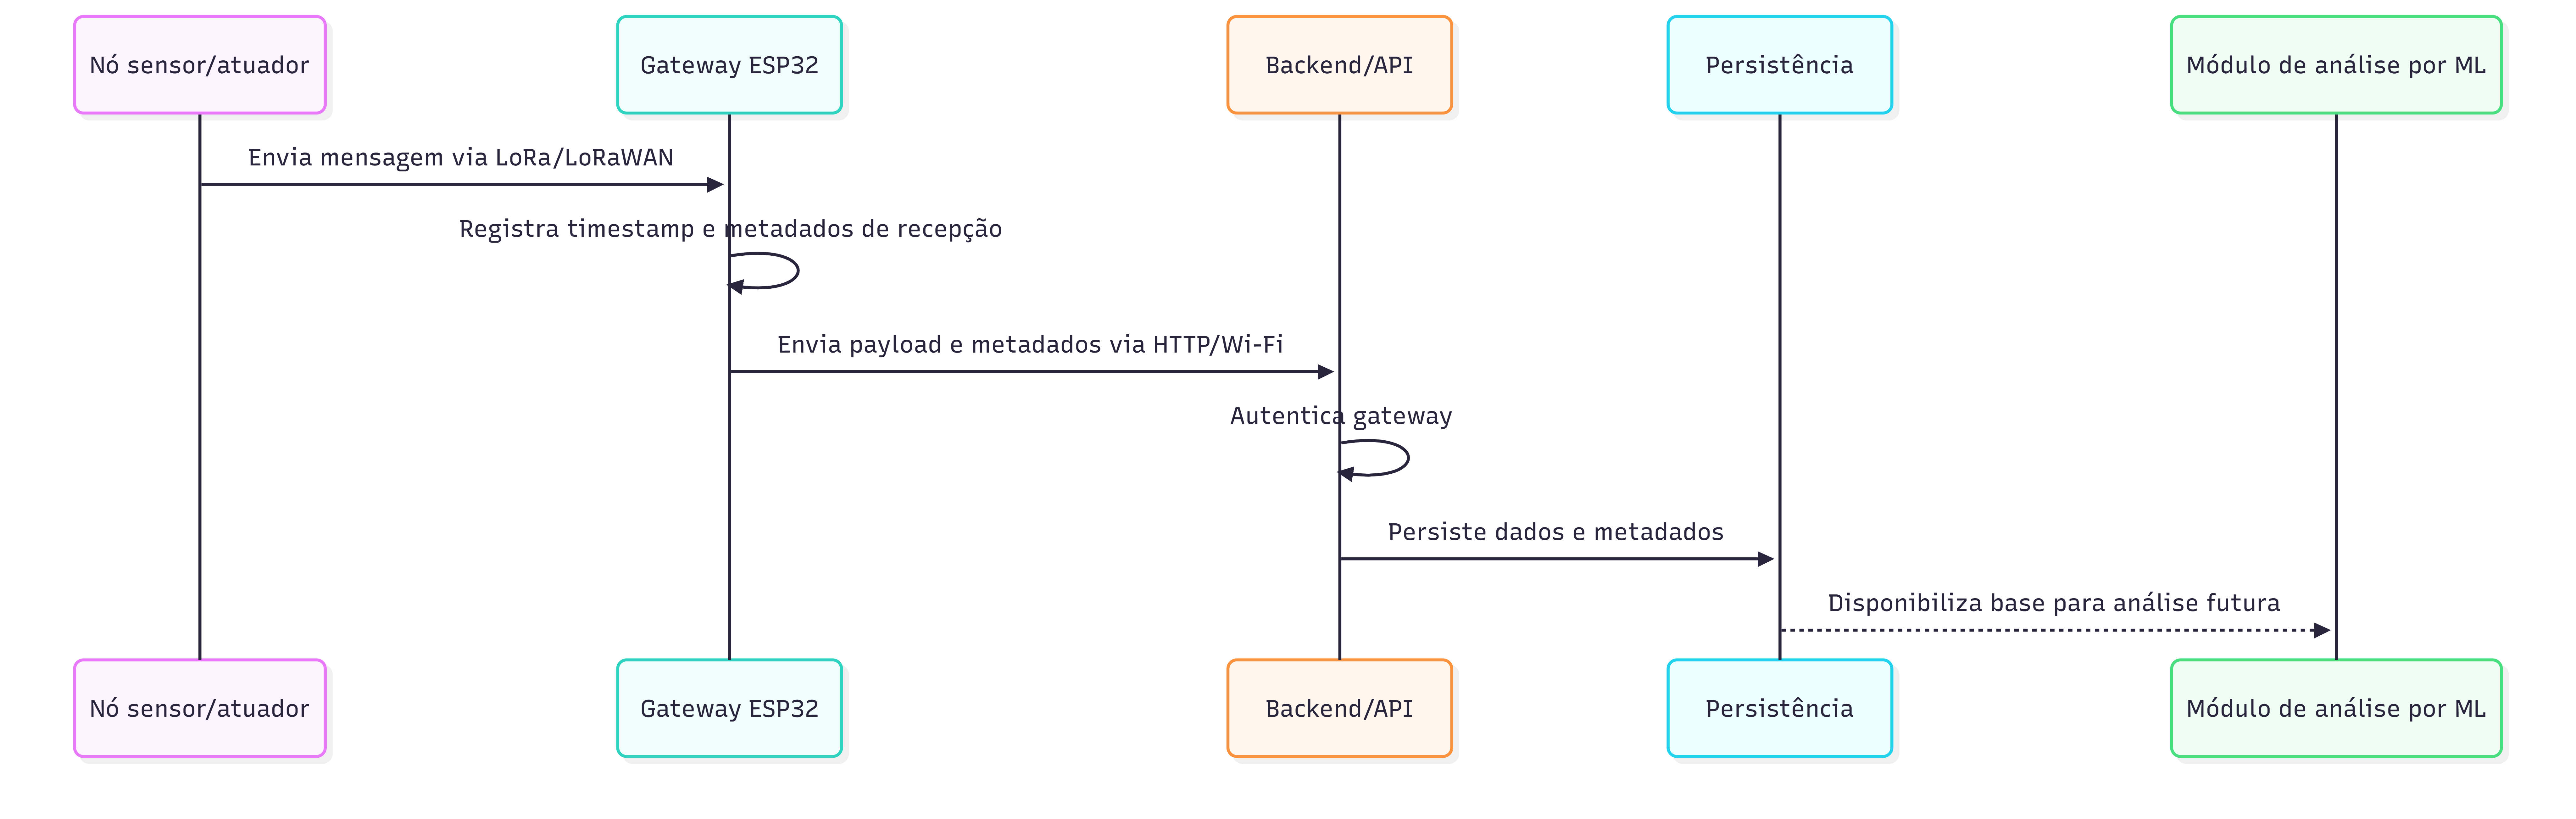
\includegraphics[scale=0.05]{barea/figuras/arch-2-uml.png}
  \end{center}

\end{figure}

Essa representação também ajuda a evidenciar que o sistema foi concebido para operar de forma orientada a evento. Em vez de depender de comunicação contínua, o fluxo é ativado pela geração e recepção das mensagens produzidas em campo, o que torna a proposta mais compatível com o tipo de aplicação e com as restrições energéticas associadas aos dispositivos embarcados.

%%%%%%%%%%%%%%%%%%%%%%%%%%%%%%%%%%%%%%%%%%%%%%%%%%%%
%%%%%%%%%%%%%%%%%%%%%%%%%%%%%%%%%%%%%%%%%%%%%%%%%%%%


\section{Especificação de Requisitos e Revisão Bibliográfica}

%%%%%%%%%%%%%%%%%%%%%%%%%%%%%%%%%%%%%%%%%%%%%%%%%%%%
\subsection{Materiais e bases de dados}
\label{subsec:ml-dataset}

Esta parte do método trata do modelo de detecção. Ela parte do RSSI, o
metadado de recepção definido na Seção~\ref{subsec:camada_fisica_lora}, e
entrega o detector que o \textit{gateway} da Seção~\ref{sec:requisitos_infra}
executa, descrito na Seção~\ref{subsec:ml-protocolo-borda}. O modelo é estimado
com o \textit{dataset} Tour Perret,
publicado pelo CampusIoT da Université Grenoble Alpes \cite{tourperret_dataset}.
Ele reúne os eventos de cinco nós sensores instalados na Tour Perret, em
Grenoble, recebidos de 25/06/2021 a 23/06/2023 por um servidor de rede
ChirpStack v3, num total de 421.937 mensagens. O arquivo usado é o oficial,
conferido pelo resumo SHA-256 publicado com ele. Cada evento de
\textit{uplink} traz uma lista com uma entrada por \textit{gateway} que recebeu
o quadro, com o RSSI medido naquele \textit{gateway} \cite{brocaarintegration}.

O \textit{dataset} vem de sensores em operação real e não tem rótulos de ataque.
Por isso ele serve para aprender o comportamento esperado do RSSI, e a
capacidade de detecção é medida com desvios sintéticos, como descrito na
Seção~\ref{subsec:ml-protocolo-deteccao}.

\subsection{Limpeza e recorte da série}
\label{subsec:ml-limpeza}
% sec:selecao_variaveis: rótulo citado pelas Seções 2.1 e 3.1 (barea); aqui se define que o modelo usa só o RSSI.
\label{sec:selecao_variaveis}

A limpeza segue regras numeradas, cada uma com a contagem de linhas depois de
aplicada, como mostram a Tabela~\ref{tab:ml-limpeza} e a
Figura~\ref{fig:ml-funil}. Os dados ficam em duas tabelas, uma de quadros e
outra de recepções, segundo o princípio de uma linha por observação
\cite{wickham2014tidy}. As regras têm quatro papéis diferentes. L1 e L4 removem
registros que não são medidas novas. L2 e L3 só organizam os dados. L6 e L8 não
removem dados inválidos. Elas fazem o recorte do estudo, escolhendo um nó
sensor e um trecho contínuo. L7 e L9 apenas marcam quadros, sem remover nada, e
L5 registra a decisão de não filtrar o RSSI.

\begin{table}[htb]
	\centering
	\caption{Regras de limpeza e recorte da série de RSSI}
	\label{tab:ml-limpeza}
	\begin{tabular}{llr}
		\hline
		\textbf{Regra} & \textbf{O que faz} & \textbf{Linhas depois} \\
		\hline
		L1 & Mantém só eventos de \textit{uplink} & 421.906 \\
		L2 & Usa o instante de arquivamento como eixo de tempo & 421.906 \\
		L3 & Separa quadros e recepções (recepções) & 3.559.119 \\
		L4 & Remove retransmissões (quadros) & 398.699 \\
		L5 & Não aplica limite físico ao RSSI & 398.699 \\
		L6 & Seleciona o nó sensor \texttt{441a1ed9} & 193.442 \\
		L7 & Marca trocas de taxa de dados e quedas do FCnt & 193.442 \\
		L8 & Seleciona o maior trecho sem lacuna maior que 1~h & 58.540 \\
		L9 & Marca os quadros sem RSSI no \textit{gateway} escolhido & 58.540 \\
		\hline
	\end{tabular}
	\legend{Fonte: elaborado pelos autores.}
\end{table}

\begin{figure}[htb]
	\centering
	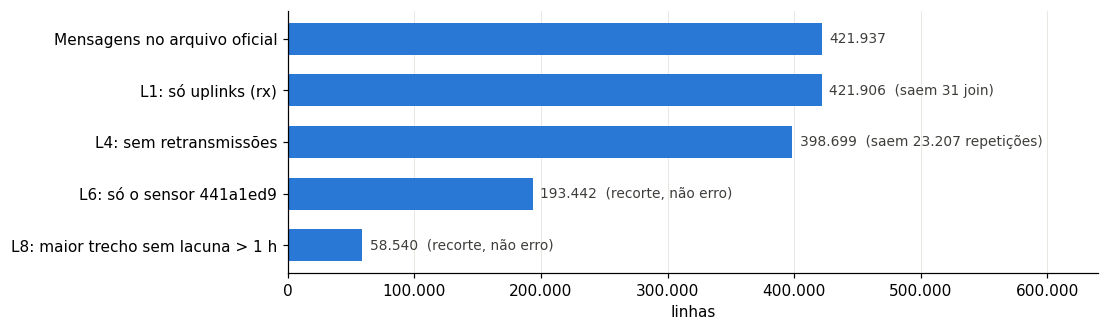
\includegraphics[width=0.85\textwidth]{tadaki/figuras/ml-funil-limpeza.png}
	\caption{Quantidade de linhas depois de cada etapa da limpeza e do recorte}
	\label{fig:ml-funil}
	\legend{Fonte: elaborado pelos autores.}
\end{figure}

A regra L4 trata como retransmissão o quadro do mesmo nó sensor com o mesmo
FCnt do anterior, recebido em menos de 60~s, porque o FCnt não sobe quando o
mesmo quadro é reenviado \cite{lorawan103}. No trecho usado, a janela de 60~s
não muda nada, pois de 10~s a sem limite são sempre as mesmas 4
retransmissões. A regra L5 deixa o RSSI sem filtro, porque no trecho usado ele
fica entre $-120$ e $-90$~dBm e um valor extremo pode trazer informação sobre o
processo \cite{hyndman2021}, que é justamente o que a detecção procura.

O estudo usa só o RSSI, de um nó sensor e de um \textit{gateway}. Entre os cinco
nós sensores, o \texttt{441a1ed9} tem ao mesmo tempo o maior número de quadros
(193.442), a taxa de dados mais estável (99,99\% em DR5, com 13 trocas) e o
maior trecho contínuo (58.540 quadros, contra no máximo 24.992 dos outros). O
\textit{gateway} \texttt{17459c66} é o de maior cobertura desse nó sensor, com
97,2\% dos quadros. O maior trecho sem intervalo acima de 3.600~s vai de
16/11/2021 a 08/06/2022, em 203,7 dias, e é o mesmo para qualquer limite entre
3.600 e 14.400~s.

\subsection{Preparação da série}
\label{subsec:ml-preparacao}

Depois da limpeza, quatro decisões transformam os quadros em uma série pronta
para o modelo. A série começa no primeiro quadro com RSSI observado, porque
antes dele não há valor anterior a repetir, o que descarta 4 quadros e deixa
58.536. O quadro que o \textit{gateway} escolhido não recebeu, 2,8\% do
trecho, recebe o último valor observado e fica marcado. Essa forma de
preencher usa só o passado. Uma alternativa medida, deixar o vazio para o
próprio modelo tratar, mudou o RMSE de validação do ARIMA por canal de
1,136 para 1,135~dBm.

O eixo da série é a ordem dos quadros, e não o relógio, porque o modelo supõe
passos iguais. O nó sensor transmite a intervalos regulares. O intervalo entre
quadros consecutivos tem mediana de 300,0~s e fica até 300,03~s em 99\% dos
casos, e só 24 dos 58.535 intervalos passam de 600~s. A divisão é cronológica,
como mostra a Tabela~\ref{tab:ml-divisao}.

\begin{table}[htb]
	\centering
	\caption{Divisão da série em treino, validação e teste}
	\label{tab:ml-divisao}
	\begin{tabular}{lrlr}
		\hline
		\textbf{Parte} & \textbf{Quadros} & \textbf{Período (UTC)} & \textbf{Sem RSSI} \\
		\hline
		Treino (70\%) & 40.975 & 16/11/2021 a 08/04/2022 & 1.355 \\
		Validação (15\%) & 8.780 & 08/04/2022 a 08/05/2022 & 121 \\
		Teste (15\%) & 8.781 & 08/05/2022 a 08/06/2022 & 138 \\
		\hline
	\end{tabular}
	\legend{Fonte: elaborado pelos autores.}
\end{table}

O treino estima os coeficientes do modelo. A validação serve a todas as
escolhas, a ordem do modelo e o limiar do alarme. O teste é usado uma única vez
para cada configuração final.

\subsection{Protocolo de avaliação da previsão}
\label{subsec:ml-protocolo}

Toda previsão é um passo à frente. Os coeficientes do ARIMA são estimados uma
vez no treino e depois aplicados, fixos, ao resto da série
\cite{statsmodelsapply}, de modo que cada quadro é previsto com os valores
reais até o quadro anterior, como faria o \textit{gateway}. A diferenciação é
decidida pelo teste KPSS no treino, a ordem é escolhida pelo RMSE na validação,
e cada configuração final é avaliada uma única vez no teste.

O erro é medido pelo RMSE e pelo MAE da Seção~\ref{subsec:ml-avaliacao} e
também pela mediana do erro absoluto, que indica o erro típico de um quadro.
As três medidas usam só os quadros com RSSI observado, porque num quadro
preenchido o \textit{random walk} acerta por construção.

O modelo é comparado com duas referências. A primeira é o \textit{random walk}
da Equação~\ref{eq:ml-random-walk}. A segunda, mais exigente, é o
\textit{random walk} por canal, que repete o último valor observado no mesmo
canal de frequência. Ganhar desta segunda referência mostra que o modelo
acrescenta algo além de separar os canais.

A robustez dos resultados é verificada de quatro formas. O mesmo procedimento é
repetido no \textit{gateway} \texttt{100210b9}. A ordem do modelo é variada um
parâmetro de cada vez, para ver se o resultado depende de uma ordem
específica. A execução completa, do \textit{dataset} bruto aos resultados, é
refeita numa cópia isolada do projeto. Por fim, para medir quanto dado de
treino basta, o ARIMA é estimado com treinos de 6~h a 142 dias, todos
terminando no fim do treino e avaliados na mesma validação. Um tamanho basta
quando o RMSE fica abaixo do \textit{random walk} por canal e no máximo 20\%
acima do obtido com o treino inteiro.

\subsection{Protocolo da detecção}
\label{subsec:ml-protocolo-deteccao}

A detecção usa a regra da Equação~\ref{eq:ml-deteccao} sobre o erro do modelo
final. Em cada canal, o limiar $\tau$ é o quantil de 99\% do erro absoluto na
validação, o que fixa cerca de 1\% de alarmes falsos sem depender da suposição
de normalidade \cite{hundman2018spacecraft}. O limiar nunca fica abaixo de
1,5~dB, porque o \textit{gateway} informa o RSSI em valores inteiros de dB.

Como o \textit{dataset} não tem ataques identificados, a detecção é medida com
desvios sintéticos, somados a uma cópia do teste. Cada desvio é um degrau de
$+\Delta$ ou $-\Delta$~dB, com $\Delta$ de 1 a 10~dB, em dois formatos, um de 12
quadros, cerca de 1~h, e outro de um só quadro. O sentido positivo segue o
efeito do \textit{jamming} reativo sobre o RSSI \cite{ruotsalainen2022jamming}.
Cada combinação é aplicada em 300 posições sorteadas do teste, uma de cada vez,
com semente fixa, e o valor alterado entra no histórico do modelo, como
aconteceria na borda. As medidas são a taxa de alarmes falsos no teste sem
desvio e a fração dos desvios com ao menos um alarme, com intervalo de
confiança de 95\% pelo método de Wilson.

Para saber quanto da detecção vem do modelo, o mesmo protocolo é aplicado a um
detector mais simples, que usa como previsão o \textit{random walk} por canal.
Como o RSSI é inteiro, o erro desse detector também é inteiro, e o limiar por
quantil não consegue fixar o alarme falso em 1\%. Por isso ele é avaliado em
duas versões. A primeira usa a mesma regra, o que dá menos alarmes falsos que o
ARIMA, e a segunda usa o limiar um valor inteiro abaixo, o que dá mais.

\subsection{Execução do detector no microcontrolador}
\label{subsec:ml-protocolo-borda}

Com os coeficientes fixos, a previsão um passo à frente do ARIMA$(0,1,1)$ é a
suavização exponencial simples \cite{hyndman2021}, como na
Equação~\ref{eq:ml-borda}, em que $\alpha = 1 + \theta$ e $\theta$ é o
coeficiente de média móvel estimado no treino de cada canal.
\begin{equation}
	\hat{y}_{t+1} = \hat{y}_t + \alpha \left( y_t - \hat{y}_t \right)
	\label{eq:ml-borda}
\end{equation}

Por isso o detector não precisa de biblioteca de séries temporais. Para cada
canal ele guarda $\alpha$, o limiar e a última previsão. Esses valores são
exportados do Python para um arquivo de cabeçalho em C++, e o mesmo código é
compilado para o computador e para a placa Heltec WiFi LoRa 32 V3, com ESP32-S3,
usada pela frente de infraestrutura. A conferência compara, quadro a quadro,
a previsão e o alarme do detector com os do Python, na série de teste e na mesma
série com um desvio sintético de $+5$~dB por 12 quadros. No \textit{gateway} do
protótipo, o detector roda depois do registro de cada quadro autenticado, sem
alterar o dado registrado, e um botão da placa soma um desvio sintético ao RSSI
que o detector recebe, para simular um ataque.



\subsection{Biblioteca Ascon}
\label{subsec:biblioteca-ascon}
Para a implementação das primitivas criptográficas no microcontrolador, optou-se pela utilização da biblioteca de código aberto \textit{ascon-suite}, mantida por \citeonline{weatherley2023ascon}. A escolha desta implementação específica, em detrimento do repositório de referência matemático original (\textit{ascon-c}), justifica-se por fatores arquiteturais estritamente alinhados aos objetivos de prototipagem em sistemas embarcados.

Primeiramente, a \textit{ascon-suite} foi estruturada com foco em plataformas com restrição de recursos, fornecendo rotinas de \textit{backend} altamente otimizadas em linguagem \textit{Assembly}, podendo ser usada diretamente na IDE do Arduino como uma biblioteca, facilitando o desenvolvimento na placa ESP32.

Em segundo lugar, a biblioteca expõe, além da interface de uma única chamada, uma API incremental que permite cifrar mensagens em fragmentos sucessivos, mantendo apenas o estado interno de 80 bytes entre as chamadas. Esse recurso não é exigido pelos \textit{payloads} deste trabalho, que cabem integralmente em memória, mas amplia a margem de crescimento da solução para mensagens maiores que a RAM disponível.

Por fim, o rigor técnico da biblioteca possui forte validação científica. Os códigos otimizados em \textit{Assembly} e C que deram origem à \textit{ascon-suite} foram empregados como base metodológica para a extração de métricas de desempenho em microcontroladores durante o processo de padronização do NIST, com resultados documentados na seção 4.1.3 do relatório oficial NIST IR 8454 \cite{nistir8454}. Uma das três plataformas de teste ali utilizadas é o ESP32 (Xtensa LX6, 240~MHz), o mesmo microcontrolador e a mesma frequência adotados neste trabalho.

A implementação utilizada neste trabalho, fornecida pela biblioteca ascon-suite, corresponde à versão finalista submetida à competição de Criptografia Leve do NIST (Ascon v1.2), e não à forma normatizada posteriormente na publicação SP 800-232 (2025). Especificamente, adota-se a variante Ascon-128a, que compartilha a mesma estrutura de permutação do Ascon-AEAD128 padronizado. As diferenças entre a v1.2 e o SP 800-232 concentram-se no vetor de inicialização, na ordenação de bytes na interface de entrada/saída e na separação de domínio. Como o custo computacional do Ascon é dominado pelas aplicações da permutação, idênticas nas duas versões, espera-se que as métricas de desempenho, memória e energia sejam essencialmente equivalentes.

%%%%%%%%%%%%%%%%%%%%%%%%%%%%%%%%%%%%%%%%%%%%%%%%%%%%
%%%%%%%%%%%%%%%%%%%%%%%%%%%%%%%%%%%%%%%%%%%%%%%%%%%%


\section{Testes e Avaliação de Desempenho (\textit{Benchmarking})}
\label{subsec:validacao-ascon}
\subsection{\textit{Known Answer Tests} (KAT)}
A primeira etapa é a validação através dos \textit{Known Answer Tests} (KAT), que são testes disponibilizados pelo próprio grupo que desenvolveu o Ascon. Eles fornecem parâmetros de entrada específicos que devem resultar em saídas exatas e já esperadas. Como o trabalho utiliza a variante Ascon-128a (versão 1.2), a validação emprega os vetores de teste correspondentes a essa versão, distribuídos junto à própria \textit{ascon-suite} e derivados do repositório de referência \textit{ascon-c} \cite{ascon_reference_c}.

Para validar a biblioteca de forma puramente matemática, os testes são rodados exaustivamente em um computador desktop. Depois, para garantir que não haja nenhuma anomalia de compilação ou diferença causada pela arquitetura de hardware, testes adicionais são executados diretamente na placa, com um volume menor de vetores.

Como garantia extra, a validação na placa precede qualquer coleta de desempenho, de modo que as medições incidam apenas sobre uma implementação já verificada, o próprio \textit{firmware} de medição repete dois vetores do KAT, e um vetor de referência do AES-GCM, antes de medir, e interrompe a execução se algum deles falhar. Ao comparar as saídas das funções da biblioteca \textit{ascon-suite} com os resultados oficiais, comprova-se de forma prática que a implementação opera corretamente no ambiente do projeto.

%%%%%%%%%%%%%%%%%%%%%%%%%%%%%%%%%%%%%%%%%%%%%%%%%%%%

\subsection{Validação dos Dados Associados (AEAD)}
Outro teste é a validação da autenticidade do modo AEAD e a sua capacidade de rejeição de anomalias. Para avaliar a resiliência do sistema contra um ataque de \textit{Man-in-the-middle} (MitM), no qual um interceptador tenta forjar ou corromper a mensagem em trânsito, a metodologia emprega a técnica de injeção intencional de falhas (\textit{bit-flipping}).

Após a geração de um pacote válido, o firmware de teste altera intencionalmente bits específicos antes de repassar a mensagem para a função de decifragem. A adulteração é testada em três frentes distintas.
\begin{itemize}
\item \textbf{No texto cifrado (\textit{Ciphertext}):} simulando um atacante que tenta alterar o valor do \textit{payload} do sensor.
\item \textbf{Nos Dados Associados (AD):} alterando o cabeçalho do protocolo LoRaWAN, simulando uma tentativa de modificar metadados de roteamento ou de identificação do nó.
\item \textbf{Na \textit{Tag} de Autenticação:} simulando um cenário onde a mensagem é modificada e o atacante anexa uma assinatura forjada ou corrompida.
\end{itemize}

O resultado esperado em todos os cenários de adulteração é que a função de decifragem do algoritmo reconheça a quebra de integridade e falhe imediatamente, retornando um código de erro e garantindo que nenhum fragmento do texto claro modificado seja entregue para a camada de aplicação do microcontrolador.

%%%%%%%%%%%%%%%%%%%%%%%%%%%%%%%%%%%%%%%%%%%%%%%%%%%%

\subsection{Vazamento de Memória e Ataques de Canal Colateral}
A avaliação de desempenho não se limita à validação funcional e engloba também o consumo de memória (RAM) e o tempo de execução. Para a análise de memória, a metodologia emprega as funções nativas do ESP-IDF. O uso do \textit{Heap} é monitorado por meio da função \texttt{esp\_get\_free\_heap\_size()} antes e depois da execução e, durante a execução, por uma tarefa no segundo núcleo do processador que lê o \textit{heap} livre continuamente e registra o menor valor observado, de modo a detectar alocações feitas e liberadas dentro da própria operação, invisíveis à comparação entre o antes e o depois. Adicionalmente, mede-se a profundidade máxima alcançada na Pilha (\textit{Stack}) através da função \texttt{uxTaskGetStackHighWaterMark()}, lida dentro de uma tarefa dedicada à operação, uma vez que essa marca registra o ponto mais fundo já atingido pela pilha da tarefa, lida na tarefa principal ela refletiria o uso anterior de outras rotinas, e não o do algoritmo.

Outro aspecto avaliado é o espaço ocupado de memória. O procedimento consiste em compilar o firmware e analisar o uso de memória Flash, comparando os resultados do compilador com e sem a inclusão da biblioteca no projeto.

Quanto ao tempo de execução, a metodologia busca não apenas medir a eficiência, mas também validar a resistência das implementações contra ataques de canal colateral baseados em tempo (\textit{Timing Side-Channel Attacks}). A medição extrai diretamente a quantidade de ciclos de \textit{clock} processados, lendo o contador de ciclos da CPU do ESP32 por meio da função \texttt{ESP.getCycleCount()}, para a cifragem e para a decifragem, em \textit{payloads} de 0, 2, 16, 23, 32 e 64 bytes. Os múltiplos de 16 bytes sustentam o modelo linear de custo por bloco, o \textit{payload} vazio mede a parcela fixa diretamente, e 2 e 23 bytes correspondem aos dois tamanhos de mensagem que ocorrem no \textit{dataset} Tour Perret, usado pela frente de aprendizado de máquina. Em cada tamanho é tomado o piso, o menor valor de 2.000 medidas, com as interrupções habilitadas, de modo que Ascon e AES sejam medidos exatamente da mesma forma. O \textit{driver} de AES do ESP-IDF já protege a operação de bloco com uma seção crítica própria \cite{espressif2026idf}, e o piso de 2.000 medidas faz o papel de filtro contra as interrupções que atingem o restante da chamada. Para o Ascon, o piso com as interrupções desabilitadas é medido como contraprova. Para validar a mitigação de ataques de canal colateral, são realizados testes repetitivos enviando cargas de dados (\textit{payloads}) com conteúdos e chaves completamente distintos, mas de tamanhos idênticos, incluindo classes de entrada fixas (todos os bytes nulos, todos 0xFF, alternados) e variáveis (rampa e valores derivados de um \textit{hash}), na linha do método dudect, que compara o tempo entre classes de entrada em vez de confiar numa única distribuição \cite{reparaz2017dudect}. O resultado esperado é que a variação nos ciclos de \textit{clock} consumidos seja desprezível, coerente com o projeto do algoritmo. A camada de substituição do Ascon dispensa tabelas de consulta, o que afasta ataques de temporização por cache \cite{ascon_v12_spec}. Dessa forma, o tempo de processamento do nó sensor não permite ao atacante deduzir fragmentos da chave ou da mensagem.

Por fim, para verificar a reprodutibilidade, o procedimento é repetido em 100 execuções independentes por tamanho de \textit{payload}, registrando-se o piso de ciclos (o menor valor medido) de cada execução, nas duas placas do projeto, o ESP32 clássico e o ESP32-S3 da placa Heltec com LoRa. A análise distingue a variação entre execuções, dada pela dispersão dos pisos, da variação interna a cada execução, dada pelo desvio padrão de suas medidas. O mesmo se aplica ao comparativo com o AES-128-GCM, tomando como métrica a razão entre os pisos, que cancela fatores comuns às duas medições.

%%%%%%%%%%%%%%%%%%%%%%%%%%%%%%%%%%%%%%%%%%%%%%%%%%%%

\subsection{Avaliação de Consumo Energético}
\label{subsec:energia_metodo}
A avaliação restringe-se ao custo energético das operações criptográficas, não incluindo o consumo da transmissão via rádio. A medição é realizada através da técnica de monitoramento da queda de tensão em um resistor de precisão (\textit{shunt}) de 1$\Omega$ conectado em série com a alimentação de 3,3V do microcontrolador \cite{hubble2024esp32power}, conforme a Figura~\ref{fig_setup_consumo}. As capturas são feitas com um osciloscópio digital, utilizando um pino GPIO como sinal de gatilho (\textit{trigger}) para delimitar com precisão o intervalo de tempo exato da execução das funções criptográficas.

Considerando que o módulo \textit{ESP32 DevKitV1} possui componentes periféricos que consomem corrente de forma constante, como o LED de operação, o regulador de tensão LDO e o conversor USB-Serial, a análise não foca no consumo absoluto da placa. Em vez disso, é aplicada a metodologia de Diferença de Consumo ($\Delta$), na qual subtrai-se a corrente de repouso (\textit{baseline}) do sistema ocioso do valor obtido durante o processamento do algoritmo.

Uma operação isolada não é mensurável dessa forma. A cifragem de 23 bytes dura cerca de 27~$\mu$s, e um acréscimo de poucos miliampères nesse intervalo desaparece no ruído da corrente de repouso da placa, da ordem de 50~mA, com a resolução de 8 bits do osciloscópio. Por isso cada operação é repetida 20.000 vezes em sequência, com o pino de gatilho em nível alto durante toda a rajada, que dura de meio segundo a dois segundos conforme o algoritmo e a placa. O osciloscópio registra a rajada inteira, e toma-se a média da tensão no resistor dentro da janela da rajada e a média em um trecho de repouso da mesma captura. A diferença entre as duas, dividida pela resistência, é a corrente que a operação acrescenta, e a energia por operação é o produto da tensão na placa, desse acréscimo e da duração da rajada, dividido pelo número de repetições. Além do Ascon-128a e do AES-128-GCM, em cifragem e decifragem, mede-se um caso de controle em que o processador apenas aguarda o mesmo tempo em um laço, para separar o custo de manter o núcleo ativo do custo do algoritmo. Durante a medição a placa é alimentada apenas pela fonte, com o cabo USB desconectado, porque o regulador da placa e o terra do cabo criariam caminhos de corrente por fora do resistor.

\begin{figure}[htb]
  \caption{\label{fig_setup_consumo}Configuração de medição de corrente via resistor \textit{shunt} e osciloscópio}
  \begin{center}
      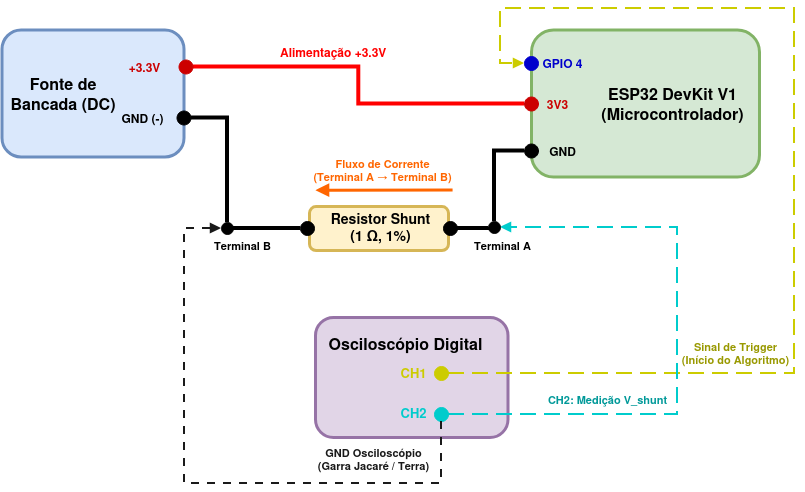
\includegraphics[scale=0.5]{felipe/figuras/setup_consumo_energia.png}
  \end{center}
  \legend{Fonte: Elaborado pelos autores (2026) com base em \cite{hubble2024esp32power}}
\end{figure}



% Capítulo 4. Especificação de Requisitos
\chapter{Especificação de Requisitos} \label{cap:especificacao}

%%%%%%%%%%%%%%%%%%%%%%%%%%%%%%%%%%%%%%%%%%%%%%%%%%%%
%%%%%%%%%%%%%%%%%%%%%%%%%%%%%%%%%%%%%%%%%%%%%%%%%%%%

\section{Especificação da arquitetura do sistema}
\label{sec:requisitos_infra}

A arquitetura especificada neste trabalho define a organização técnica da solução proposta para comunicação, encaminhamento e persistência dos dados produzidos na rede de campo. Sua função é estruturar, de forma coerente, os componentes responsáveis pela coleta das informações, pela transição entre a comunicação embarcada e a infraestrutura de aplicação, e pelo armazenamento dos dados necessários ao funcionamento do sistema e às etapas posteriores de segurança e análise.

A solução foi organizada em quatro blocos principais: nó sensor, \textit{gateway}, \textit{backend} com API e persistência. No trecho de campo, o nó coleta os dados do ambiente e transmite quadros curtos por um enlace LoRa ponto a ponto, atendendo aos requisitos de operação em dispositivos com restrição energética. O \textit{gateway} concentra em um único dispositivo os papéis que o modelo LoRaWAN distribui entre \textit{gateway}, \textit{network server} e \textit{application server}: recebe os quadros, verifica a autenticidade e a ordem, registra os metadados de recepção e encaminha as mensagens ao \textit{backend}, em conformidade com os requisitos RF3, RF6 e RF12.

A partir do \textit{gateway}, a comunicação passa a utilizar Wi-Fi e requisições HTTP, integrando a rede embarcada a uma API autenticada e a um mecanismo centralizado de persistência, implantados em infraestrutura local, na mesma rede do \textit{gateway}. Essa escolha mantém a coleta independente de conectividade externa e dispensa a negociação de certificados no dispositivo embarcado; a migração para infraestrutura em nuvem, com transporte cifrado, é tratada como extensão e discutida no Capítulo~\ref{cap:consideracoes}. A camada de aplicação permanece disponível de forma contínua para o recebimento dos dados encaminhados pelo \textit{gateway}, e o próprio \textit{gateway} mantém os quadros em memória quando a API está indisponível.

Além dos dados de aplicação, como temperatura e luminosidade, a arquitetura prevê a persistência de metadados relevantes para o acompanhamento da comunicação, incluindo informações de origem, sequência, recepção e qualidade do enlace. Essa escolha atende aos requisitos RF5 e RF7 e contribui para a rastreabilidade da operação, conforme estabelecido em RNF6. Cada registro carrega ainda o identificador da sessão em que foi recebido e a indicação de ter sido entregue em tempo real ou reenviado após uma falha de conectividade (RF9 e RF10), de modo que uma queda da rede entre \textit{gateway} e \textit{backend} nunca se confunda com perda no enlace de rádio. A mesma base persistida prepara a infraestrutura para a incorporação de mecanismos de criptografia leve e de análise por aprendizado de máquina, em conformidade com RNF7 e RNF8.

A Figura~\ref{fig:arquitetura-especificada} apresenta a arquitetura técnica especificada para o sistema. A partir dessa organização, as subseções seguintes detalham os requisitos funcionais e não funcionais da infraestrutura proposta, que fundamentam e justificam as decisões arquiteturais adotadas.

\begin{figure}[htb]
  \caption{\label{fig:arquitetura-especificada}Arquitetura especificada do sistema proposto.}
  \begin{center}
      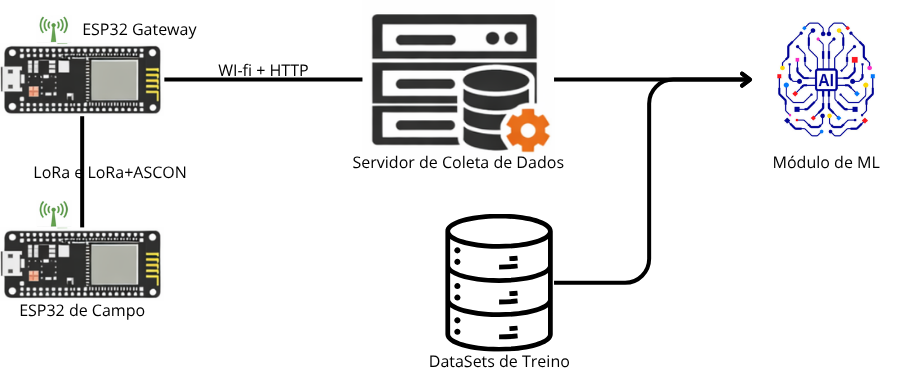
\includegraphics[scale=0.5]{barea/figuras/arch_figure1.png}
  \end{center}

\end{figure}

%%%%%%%%%%%%%%%%%%%%%%%%%%%%%%%%%%%%%%%%%%%%%%%%%%%%

\subsection{Requisitos funcionais da infraestrutura proposta}

Os requisitos funcionais da infraestrutura proposta descrevem os comportamentos esperados da arquitetura do sistema, considerando a coleta, o encaminhamento, a autenticação e a persistência das informações produzidas na rede de campo.

\begin{enumerate}
    \item[RF1.] O sistema deve permitir que os nós de campo coletem e transmitam dados de aplicação, incluindo, no protótipo previsto, informações de temperatura e luminosidade.

    \item[RF2.] Cada mensagem transmitida pelos nós deve conter, além dos dados de aplicação, informações mínimas de identificação e acompanhamento, incluindo identificador do dispositivo e contador de mensagens.

    \item[RF3.] O gateway deve receber as mensagens provenientes da rede de campo, registrar os metadados de recepção e encaminhar essas informações ao backend por meio de rede Wi-Fi e requisições HTTP.

    \item[RF4.] O backend deve autenticar as requisições enviadas pelo gateway, restringindo o recebimento de dados a dispositivos previamente autorizados.

    \item[RF5.] O sistema deve persistir os dados de aplicação recebidos dos nós juntamente com os metadados associados à comunicação.

    \item[RF6.] A infraestrutura deve permitir armazenamento temporário das mensagens no gateway em situações de indisponibilidade da conexão com o backend, com possibilidade de reenvio posterior.

    \item[RF7.] Os dados persistidos devem permanecer disponíveis para uso posterior pelas camadas de segurança e de análise por aprendizado de máquina.

    \item[RF8.] O gateway deve registrar cada quadro recebido em sua interface serial, em formato legível por máquina, independentemente do estado da conexão com o backend, de modo que a coleta nunca dependa da rede.

    \item[RF9.] O sistema deve identificar sessões de operação, de modo que quadros recebidos após um reinício do nó ou do gateway não sejam confundidos com a continuação da sequência anterior.

    \item[RF10.] Cada quadro persistido deve indicar sua origem: entregue em tempo real, reenviado a partir do armazenamento temporário do gateway ou relido de um registro serial.

    \item[RF11.] O gateway deve emitir periodicamente um sinal de vida com contadores de quadros recebidos, rejeitados e encaminhados, para distinguir ausência de tráfego de falha do próprio gateway.

    \item[RF12.] O gateway deve descartar, sem encaminhar, quadros com tamanho diferente do esperado, com falha de verificação de integridade, com falha de autenticação ou com contador não crescente, contabilizando cada caso separadamente.

\end{enumerate}

%%%%%%%%%%%%%%%%%%%%%%%%%%%%%%%%%%%%%%%%%%%%%%%%%%%%

\subsection{Requisitos não funcionais da infraestrutura proposta}

Os requisitos não funcionais da infraestrutura proposta descrevem propriedades de operação e restrições que devem ser observadas para que a solução seja compatível com o contexto de sistemas embarcados e Internet das Coisas. Para sua elicitação e organização, adotou-se como referência a norma ISO/IEC 25010, considerando principalmente características relacionadas à eficiência de desempenho, confiabilidade, compatibilidade, manutenibilidade e segurança.

\begin{enumerate}
    \item[RNF1.] A infraestrutura deve ser compatível com a operação de nós de campo com restrições de energia, priorizando baixo consumo no trecho embarcado da comunicação.

    \item[RNF2.] A comunicação do sistema deve ser orientada a evento, evitando transmissões contínuas desnecessárias entre os componentes.

    \item[RNF3.] A arquitetura deve manter separação clara entre a rede de campo, baseada em LoRa ponto a ponto, e a infraestrutura de aplicação, baseada em Wi-Fi e HTTP, de modo que a recepção de rádio nunca aguarde a rede.

    \item[RNF4.] O protótipo deve preservar simplicidade de integração entre hardware, comunicação e backend, de modo a manter viável sua montagem e evolução no contexto do projeto.

    \item[RNF5.] A infraestrutura deve apresentar robustez básica a falhas temporárias de conectividade entre gateway e backend.

    \item[RNF6.] O sistema deve garantir rastreabilidade das mensagens recebidas, por meio do registro de dados e metadados que permitam identificar origem, sequência, instante de recepção e condições básicas do enlace.

    \item[RNF7.] A arquitetura deve ser compatível com a incorporação posterior de mecanismos de criptografia leve sem exigir reformulação completa da infraestrutura de comunicação.

    \item[RNF8.] A infraestrutura deve ser compatível com o uso posterior de técnicas de aprendizado de máquina aplicadas à análise do comportamento da rede e à detecção de anomalias.
    
    \item[RNF9.] O quadro transmitido não deve exceder 51 bytes, limite do plano regional AU915 na taxa de dados mais lenta, de modo que possa ser transmitido em qualquer fator de espalhamento.

    \item[RNF10.] Os metadados de recepção registrados devem ter os mesmos campos e a mesma semântica das variáveis candidatas dos modelos de detecção, permitindo comparar a coleta própria com o conjunto de dados de referência sem transformação adicional.

    \item[RNF11.] O envio ao backend não deve bloquear a recepção de rádio: um quadro que chegue durante uma requisição HTTP em andamento deve ser recebido e registrado normalmente.

\end{enumerate}

%%%%%%%%%%%%%%%%%%%%%%%%%%%%%%%%%%%%%%%%%%%%%%%%%%%%

\subsection{Rastreabilidade dos requisitos da infraestrutura}
\label{subsec:rastreabilidade_infra}

A Tabela~\ref{tab:rastreabilidade_infra} relaciona cada requisito ao componente que o atende e à forma como foi verificado. Os detalhes de implementação estão no Capítulo~\ref{cap:desenvolvimento}. As evidências vêm das quatro coletas em bancada (23 de agosto, 24 de setembro, 8 de outubro e 12 a 13 de outubro de 2026), das cinco suítes de teste executadas nas placas e dos testes automatizados do \textit{backend}. Dois requisitos estão atendidos apenas em parte e são declarados como tal: o RF1, porque os dados de aplicação ainda são sintéticos; e o RNF1, porque o nó ainda não entra em modo de baixo consumo entre transmissões. O RF6, declarado parcial até outubro, foi exercitado em uma queda real de rede em 13 de outubro.

\begin{table}[!htbp]
\centering
\caption{Rastreabilidade dos requisitos da infraestrutura}
\label{tab:rastreabilidade_infra}
\footnotesize
\begin{tabular}{lp{5,2cm}p{8cm}}
\hline
\textbf{Req.} & \textbf{Onde é atendido} & \textbf{Como foi verificado} \\
\hline
RF1  & Firmware do nó; 4 bytes de dados no quadro & Quatro coletas, de 23/08 a 13/10; dados sintéticos (parcial) \\
RF2  & Cabeçalho do quadro: identificador e contador & Suítes do quadro v2 (14 casos) e v3 (14 casos) na placa; coletas \\
RF3  & Gateway: recepção no núcleo 1, envio HTTP no núcleo 0 & 6.007 quadros recebidos em 12 a 13/10, 2.432 entregues ao vivo \\
RF4  & Token no cabeçalho HTTP, comparação em tempo constante & Testes automatizados do backend \\
RF5  & Banco SQLite com os 12 campos e metadados de ingestão & Testes; conferência serial contra banco \\
RF6  & Fila e armazenamento temporário de 512 registros no gateway & Queda real do Wi-Fi em 13/10: 512 retidos, os mais antigos descartados como previsto \\
RF7  & API de consulta e exportação em CSV & Ferramenta de análise; notebooks \\
RF8  & Registro serial sob exclusão mútua, anterior ao envio & Coleta de 23/08 sem backend; 3.575 quadros recuperados do registro em 13/10 \\
RF9  & Identificador de sessão: sorteio na inicialização mais contador de sessão & Suíte do gateway na placa; uma sessão distinta por coleta \\
RF10 & Campo de origem por idade do registro na entrega & 13/10: 2.432 ao vivo e 3.575 relidos do registro serial, distinguidos no banco \\
RF11 & Sinal de vida a cada 30 s na serial e na API & Registro serial; 669 sinais de vida no banco desde 08/10 \\
RF12 & Verificação de tamanho, CRC, anti-replay e tag & Suítes v2 e v3 na placa: forjado, repetido e contador alto rejeitados; 0 rejeições indevidas em 6.468 quadros \\
RNF1 & Potência de 5 dBm; nó sem modo de repouso & Parcial: repouso entre transmissões pendente \\
RNF2 & Recepção por interrupção; transmissão periódica & Coletas \\
RNF3 & Dois núcleos com fila de espera zero & 0 perdas em 6.007 quadros com a tarefa de rede ativa \\
RNF4 & Contrato único compartilhado pelos dois firmwares & Compilação; testes \\
RNF5 & Armazenamento temporário e espera exponencial de 1 a 30 s & Queda de 13/10: gateway seguiu recebendo e tentando reenviar por 5 h \\
RNF6 & 12 campos mais identificadores de gateway, sessão e instante UTC & Conferência serial contra banco \\
RNF7 & Dois caminhos de cifra, selecionados em tempo de compilação & AES-GCM no ar em 24/09; Ascon-128a no ar desde 08/10 \\
RNF8 & Mesmos campos das variáveis candidatas dos modelos & Análise das coletas \\
RNF9 & Quadro de 26 bytes; verificação em tempo de compilação & Compilação \\
RNF10 & Formatação byte a byte do registro & Suíte do gateway na placa (16 casos, 17/11); ETL compara coleta própria e Tour Perret sem conversão \\
RNF11 & Fila entre núcleos com espera zero & 0 perdas em 6.007 quadros com envio HTTP concorrente \\
\hline
\end{tabular}
\legend{Fonte: elaborado pelos autores (2026).}
\end{table}


%%%%%%%%%%%%%%%%%%%%%%%%%%%%%%%%%%%%%%%%%%%%%%%%%%%%
%%%%%%%%%%%%%%%%%%%%%%%%%%%%%%%%%%%%%%%%%%%%%%%%%%%%


\section{Requisitos de Segurança do Sistema criptográfico}
\label{sec:requisitos_seguranca}
\subsection{Segurança do Ascon-AEAD128 e da variante Ascon-128a}
A camada criptográfica especificada nesta seção é adicional à proteção já oferecida pelo protocolo de comunicação. A especificação do LoRaWAN determina que o \textit{payload} de aplicação seja cifrado fim a fim entre o dispositivo e o \textit{Application Server}, mas registra que a proteção de integridade não é fim a fim. O \textit{Network Server} pode alterar o conteúdo cifrado em trânsito, ainda que sem conseguir lê-lo, uma vez que detém a chave empregada no cálculo do código de integridade das mensagens. Por esse motivo, a própria norma recomenda que aplicações que exijam confidencialidade e integridade fim a fim empreguem soluções de segurança adicionais \cite{lorawan104}. É essa lacuna de integridade que a camada baseada em Ascon preenche neste trabalho.

Para o uso seguro da cifra, este trabalho adota os requisitos operacionais especificados pelo NIST para o Ascon-AEAD128 \cite{nist800232}. Embora a implementação utilizada corresponda à variante Ascon-128a (versão 1.2), esses requisitos são adotados de forma conservadora como limites aplicáveis, uma vez que as duas versões compartilham os parâmetros da Tabela~\ref{tab:parametros_ascon}. A geração da chave segue o SP 800-133r2 \cite{barker2020nist133} e emprega o mecanismo CTR\_DRBG especificado no SP 800-90A \cite{barker2015nist90a}. A aprovação refere-se ao mecanismo, e este trabalho não avaliou a conformidade da implementação utilizada. Os requisitos estão organizados em funcionais e não funcionais.

\subsubsection{Requisitos funcionais}

\begin{enumerate}
    \item[RF-S1.] A implementação da biblioteca \textit{ascon-suite} deve ser validada previamente, conforme discutido na Seção \ref{subsec:validacao-ascon}.

    \item[RF-S2.] A geração da chave criptográfica deve seguir o SP 800-133r2 \cite{barker2020nist133}, adotando a operação $K = U \oplus V$, em que $U$ é uma cadeia de bits extraída de um gerador de bits aleatórios (RBG, \textit{Random Bit Generator}) aprovado, com força de segurança de no mínimo 128 bits \cite{nist800232}, e $V$ é uma sequência gerada independentemente de $U$, que pode ser composta inteiramente por zeros.

    \item[RF-S3.] O sistema deve utilizar um Gerador Determinístico de Bits Aleatórios (DRBG - \textit{Deterministic Random Bit Generator}) através do mecanismo CTR\_DRBG para a geração de chaves criptográficas.

    \item[RF-S4.] A implementação deve fazer uso da biblioteca nativa \textit{mbedTLS} do ESP32 para extrair a entropia do periférico de \textit{hardware} (TRNG, \textit{True Random Number Generator}), nas condições em que o fabricante a garante \cite{espressif2026random}, e processá-la através do algoritmo CTR\_DRBG.

    \item[RF-S5.] A renovação da chave de um nó deve ser feita por novo provisionamento, onde descarta-se o estado criptográfico do dispositivo, gera-se nele uma chave nova, nas condições do RF-S2 ao RF-S4, e atualiza-se o registro correspondente no receptor. A chave nova deve ser gerada de forma independente da anterior, sem derivar dela nem ser transportada sob sua proteção, como exige o SP 800-133r2 para a substituição de chave comprometida \cite{barker2020nist133}. Como os gatilhos preventivos de renovação (RNF-S3 e RNF-S4) são inalcançáveis na operação prevista, conforme discutido ao final desta seção, a renovação é um procedimento de resposta a um incidente, e não de rotina.

    \item[RF-S6.] Cada nó sensor deve possuir uma chave criptográfica própria, gerada e provisionada individualmente, de modo que o comprometimento físico de um nó não exponha o tráfego dos demais. Como a exigência de unicidade do \textit{nonce} se aplica a uma mesma chave, essa separação também restringe o escopo dessa garantia a um único dispositivo \cite{nist800232}.

    \item[RF-S7.] A unicidade do \textit{nonce} exigida pelo RNF-S2 deve ser assegurada por um contador monotônico mantido em memória não volátil no próprio dispositivo, incrementado a cada operação de cifragem e persistido antes da transmissão da mensagem correspondente, de modo que uma interrupção de energia descarte valores em vez de repeti-los. Após uma reinicialização, a leitura do valor persistido deve preceder qualquer operação criptográfica. O contador não deve ser derivado de valores mantidos pela pilha de comunicação, para que a garantia de unicidade não dependa de decisões tomadas em outra camada.

    \item[RF-S8.] A camada criptográfica deve detectar e rejeitar qualquer alteração da mensagem em trânsito, seja no texto cifrado, nos dados associados ou na própria \textit{tag} de autenticação. Em caso de falha na verificação de integridade, a decifragem deve retornar erro sem entregar à aplicação qualquer fragmento de texto claro \cite{nist800232}. Este requisito responde à lacuna de integridade descrita no início desta seção.

    \item[RF-S9.] O receptor deve recusar mensagens cujo \textit{nonce} já tenha sido aceito, mantendo registro do maior valor recebido de cada dispositivo e descartando valores repetidos ou regressivos. O modo AEAD garante integridade, mas não frescor, um pacote válido retransmitido sem alteração é legítimo do ponto de vista criptográfico, e sua detecção depende de estado mantido no receptor. Este requisito complementa o RF-S7, que assegura a unicidade do \textit{nonce} na origem, estendendo a garantia ao destino.
\end{enumerate}

\subsubsection{Requisitos não funcionais}

\begin{enumerate}
    \item[RNF-S1.] A entropia bruta extraída diretamente do \textit{hardware} não deve ser utilizada sem tratamento adicional, uma vez que pode conter vícios físicos (\textit{bias}), tornando indispensável um estágio secundário de condicionamento algorítmico \cite{turan2018nist90b}.

    \item[RNF-S2.] A chave criptográfica deve ser mantida em sigilo e não deve ser empregada para outras finalidades, aliada à garantia de unicidade do \textit{nonce} para cada operação de cifragem \cite{nist800232}.

    \item[RNF-S3.] Para \textit{tags} de autenticação cujo tamanho $\lambda$ (em bits) satisfaça a condição $64 \leq \lambda \leq 128$, a quantidade de falhas de decifragem não deve exceder $2^{\lambda - 32}$.

    \item[RNF-S4.] O volume máximo de dados processados durante as rotinas de cifragem e decifragem, incluindo o \textit{nonce}, não deve ultrapassar $2^{54}$ bytes para uma mesma chave, devendo a chave ser obrigatoriamente renovada caso esse limite seja atingido. A chave também deve ser renovada quando o número de falhas de decifragem alcançar o limite estabelecido no RNF-S3 \cite{nist800232}.

    \item[RNF-S5.] A \textit{tag} de autenticação deve ser utilizada em seu comprimento integral de 128 bits, não se aplicando a este trabalho a opção de truncamento prevista no padrão. Caso venha a ser adotada, o comprimento truncado não deve ser inferior a 32 bits, valores abaixo de 64 bits exigem análise de risco prévia, e o comprimento escolhido deve permanecer constante durante toda a vida útil da chave \cite{nist800232}.

    \item[RNF-S6.] A operação de cifragem não deve realizar alocação dinâmica de memória, de modo a evitar fragmentação de \textit{heap} em dispositivos que operam por longos períodos sem reinicialização.

    \item[RNF-S7.] O consumo de memória da operação de cifragem deve ser constante e independente do tamanho do \textit{payload}, restringindo-se ao estado interno do algoritmo.

    \item[RNF-S8.] A latência de cifragem deve ser desprezível frente ao tempo de transmissão da mensagem correspondente, de modo que a camada criptográfica não se torne fator limitante do ciclo de operação do nó.

    \item[RNF-S9.] O tempo de execução da cifragem deve ser independente do conteúdo dos dados e da chave, para entradas de mesmo comprimento.
\end{enumerate}

Diante desses requisitos, alguns deles possuem impacto prático reduzido no contexto deste projeto. Como as redes LoRaWAN operam com taxas de transmissão extremamente baixas e pacotes pequenos, atingir o limite de $2^{54}$ bytes processados sob uma mesma chave é inviável durante a vida útil física do dispositivo. Da mesma forma, considerando o uso de uma \textit{tag} de 128 bits, o limite tolerado antes da obrigatoriedade de rotação da chave é de $2^{96}$ falhas de decifragem. Alcançar esse volume de tentativas de ataques de injeção na rede é improvável, dadas as severas restrições de tempo de transmissão inerentes ao protocolo.

\subsubsection{Rastreabilidade}
O Quadro~\ref{qua:rastreabilidade_ascon} relaciona cada requisito à seção do Capítulo~\ref{cap:desenvolvimento} que o verifica e à forma de verificação. Os requisitos RNF-S3 e RNF-S4 não têm verificação experimental, porque seus limites são inalcançáveis na operação prevista, como discutido acima. Os requisitos atendidos pela biblioteca \textit{AsconSecure}, do RF-S2 ao RF-S7, o RF-S9, o RNF-S1, o RNF-S2 e o RNF-S5, foram verificados por inspeção do código, e os demais por ensaio. A biblioteca encerra o uso da chave ao fim do contador de 32 bits, o que corresponde a menos de $2^{40}$ bytes processados com pacotes de até 220 bytes, 200 de \textit{payload} mais os 20 de contador e \textit{tag}, o tamanho máximo na configuração padrão da biblioteca, muito antes do limite de $2^{54}$.

\begin{quadro}[htb]
\centering
\caption{Rastreabilidade dos requisitos de segurança}
\label{qua:rastreabilidade_ascon}
\small
\begin{tabular}{lp{3,4cm}>{\raggedright\arraybackslash}p{7,6cm}}
\hline
\textbf{Requisito} & \textbf{Onde} & \textbf{Verificação} \\
\hline
RF-S1 & Seção~\ref{subsec:kat_resultados} & 1.089 vetores oficiais no computador e subconjunto na placa, sem falhas \\
RF-S2 a RF-S4 & Seção~\ref{subsec:asconsecure} & Chave gerada no nó pelo CTR\_DRBG da \textit{mbedTLS}, semeado pelo gerador de \textit{hardware}, por inspeção do código do provisionamento \\
RF-S5 & Seção~\ref{subsec:asconsecure} & Renovação por descarte do estado e novo provisionamento, sem chave no ar \\
RF-S6 & Seção~\ref{subsec:asconsecure} & Uma chave por nó, e o receptor guarda uma por nó registrado \\
RF-S7 & Seção~\ref{subsec:asconsecure} & Contador na memória não volátil (NVS) reservado em blocos de 32 antes do uso, independente do contador de quadros \\
RF-S8 & Seções~\ref{subsec:aead_resultados} e \ref{subsec:asconsecure} & 4.907 adulterações rejeitadas em cada uma das duas placas, nenhum byte de texto claro entregue \\
RF-S9 & Seção~\ref{subsec:asconsecure} & Receptor descarta contador igual ou menor que o último aceito, gravado antes da entrega \\
RNF-S1 & Seção~\ref{subsec:asconsecure} & Entropia bruta condicionada pelo CTR\_DRBG \\
RNF-S2 & Seção~\ref{subsec:asconsecure} & Chave na NVS do nó, em claro, apagada da RAM ao ser descartada, e \textit{nonce} único pelo contador. O sigilo depende do controle físico do dispositivo \\
RNF-S3, RNF-S4 & esta seção & Limites inalcançáveis na operação, sem verificação experimental \\
RNF-S5 & Seção~\ref{subsec:asconsecure} & \textit{Tag} de 128 bits, sem truncamento \\
RNF-S6 & Seção~\ref{subsec:memoria_tempo} & \textit{Heap} livre lido continuamente durante a operação, nenhuma alocação nas duas placas \\
RNF-S7 & Seção~\ref{subsec:memoria_tempo} & \textit{Buffers} fixos, estado de 80 bytes, pilha de até 436 bytes \\
RNF-S8 & Seção~\ref{subsec:memoria_tempo} & 27~$\mu$s de cifragem contra cerca de 87~ms de tempo no ar \\
RNF-S9 & Seção~\ref{subsec:memoria_tempo} & Piso idêntico em cinco classes de entrada, nas duas placas \\
\hline
\end{tabular}
\legend{Fonte: elaborado pelos autores.}
\end{quadro}


\section{Requisitos do Sistema de Detecção de Anomalias}
\label{sec:requisitos_ml}

Esta seção especifica o detector de anomalias. Ele parte do RSSI que o
\textit{gateway} mede em cada quadro, um dos metadados de recepção descritos na
Seção~\ref{subsec:camada_fisica_lora} e registrados pela infraestrutura da
Seção~\ref{sec:requisitos_infra}, e complementa a autenticação da
Seção~\ref{sec:requisitos_seguranca}, que não indica de onde o sinal partiu. O
modelo é estimado e avaliado com os dados do \textit{dataset} Tour Perret.

%%%%%%%%%%%%%%%%%%%%%%%%%%%%%%%%%%%%%%%%%%%%%%%%%%%%

\subsection{Requisitos funcionais do modelo de detecção}

\begin{enumerate}

    \item[RF-M1.] O sistema deve prever o RSSI de cada quadro um passo à frente,
    a partir dos quadros anteriores do mesmo nó sensor no mesmo
    \textit{gateway}, com um modelo por canal de frequência.

    \item[RF-M2.] O sistema deve prever o RSSI com RMSE menor que o do
    \textit{random walk} por canal.

    \item[RF-M3.] O sistema deve sinalizar como anômalo o quadro cujo erro de
    previsão passa do limiar do seu canal, calibrado no conjunto de validação.

\end{enumerate}

%%%%%%%%%%%%%%%%%%%%%%%%%%%%%%%%%%%%%%%%%%%%%%%%%%%%

\subsection{Requisitos não funcionais do modelo de detecção}

\begin{enumerate}

    \item[RNF-M1.] O modelo deve atingir o desempenho do RF-M2 com no máximo 14
    dias de quadros de treino.

    \item[RNF-M2.] O modelo deve ter no máximo dois parâmetros estimados por
    canal, para caber num dispositivo de borda.

    \item[RNF-M3.] Todo resultado deve ser reproduzível a partir do
    \textit{dataset} bruto, conferido por resumo SHA-256.

\end{enumerate}

\subsection{Rastreabilidade dos requisitos de detecção}

O Quadro~\ref{qua:rastreabilidade_ml} liga cada requisito à seção do
Capítulo~\ref{cap:desenvolvimento} em que ele é verificado.

\begin{quadro}[htb]
	\centering
	\caption{Rastreabilidade dos requisitos do modelo de detecção}
	\label{qua:rastreabilidade_ml}
	\begin{tabular}{lll}
		\hline
		\textbf{Requisito} & \textbf{Onde é verificado} & \textbf{Situação} \\
		\hline
		RF-M1 & Seção~\ref{subsec:ml-res-frequencia} & atendido \\
		RF-M2 & Seção~\ref{subsec:ml-res-frequencia} & atendido no RMSE e no MAE \\
		RF-M3 & Seção~\ref{subsec:ml-res-deteccao} & atendido com desvios sintéticos \\
		RNF-M1 & Seção~\ref{subsec:ml-res-treino} & atendido na validação \\
		RNF-M2 & Seção~\ref{subsec:ml-res-frequencia} & atendido \\
		RNF-M3 & Seção~\ref{subsec:ml-res-serie} & atendido \\
		\hline
	\end{tabular}
	\legend{Fonte: elaborado pelos autores.}
\end{quadro}



% Capítulo 5. Desenvolvimento
\chapter{Desenvolvimento do Trabalho} \label{cap:desenvolvimento}
\section{Atividades Previstas}

\subsection{Implementação da infraestrutura}
\label{subsec:implementacao_infra}

A infraestrutura foi implementada em três componentes: o firmware do nó sensor, o firmware do \textit{gateway} e o \textit{backend} de persistência, além de ferramentas de análise. Os dois firmwares rodam em placas Heltec WiFi LoRa 32 V3 \cite{heltec_wifi_lora_32_v3}, que integram o microcontrolador ESP32-S3 e o transceptor LoRa SX1262 \cite{semtech_sx1262}. O código está em repositório público, com os registros de decisão que documentam cada escolha e as alternativas descartadas.

Os parâmetros de rádio e o formato do quadro ficam em um único cabeçalho compartilhado pelos dois firmwares. A escolha é deliberada: uma divergência de frequência, fator de espalhamento ou disposição de bytes entre nó e \textit{gateway} não produz erro de compilação nem mensagem em tempo de execução, apenas um receptor que não recebe nada. Verificações em tempo de compilação garantem que o quadro tem exatamente 26 bytes e não excede o limite de 51 bytes do plano regional.

Dois caminhos de segurança coexistem no firmware, selecionados por ambiente de compilação, com o restante do código em comum. O primeiro, de linha de base, usa AES-128-GCM com a chave de rede no cabeçalho compartilhado: o quadro leva em claro um cabeçalho de 6 bytes (versão, identificador do dispositivo e contador), autenticado como dado associado, seguido de 4 bytes cifrados e da tag de 16 bytes. O segundo, padrão desde 8 de outubro de 2026, usa o Ascon-128a pela biblioteca \textit{AsconSecure} da frente de criptografia (Subseção~\ref{subsec:asconsecure}): o cabeçalho em claro e autenticado reduz-se a 2 bytes (versão e identificador), e o pacote da biblioteca ocupa os 24 restantes, com o contador de 4 bytes, os 4 bytes cifrados e a tag de 16. Os dois quadros têm 26 bytes e o mesmo tempo no ar. No caminho Ascon a chave é de cada nó: gerada na própria placa durante o provisionamento, a partir do gerador de hardware do microcontrolador, e guardada na sua memória não volátil, sem nunca constar do código; o \textit{gateway} guarda a chave de cada nó em um arquivo fora do repositório e a escolhe pelo identificador do cabeçalho. O contador da biblioteca é o contador de quadros do registro.

O nó transmite um quadro a cada cinco segundos, com agendamento em tempo absoluto: o instante da próxima transmissão é calculado a partir do anterior, e não a partir do fim da transmissão corrente, de modo que o tempo de processamento não se acumula como atraso. O contador de quadros é persistido na memória não volátil em blocos de 32: o nó grava o teto do bloco antes de usá-lo e, ao reiniciar, retoma do próximo bloco. Alguns valores são pulados a cada reinício, mas nenhum se repete, o que preserva a unicidade do \textit{nonce} derivado do contador. A biblioteca \textit{AsconSecure} faz a mesma reserva por conta própria. Como essa gravação atrasava a transmissão dos quadros de contador múltiplo de 32, no caminho Ascon o nó cifra o quadro seguinte logo depois de cada transmissão, de modo que, no instante agendado, só o rádio trabalha; o custo é que a leitura do sensor vai ao ar com cinco segundos de idade. Os dados de aplicação (temperatura e iluminância) são, nesta etapa, sintéticos: senoides com período conhecido, o que permite verificar a decifragem no receptor por inspeção. Os metadados de recepção, que são as variáveis dos modelos, não dependem deles.

O \textit{gateway} divide o trabalho entre os dois núcleos do processador. No primeiro, uma interrupção do transceptor sinaliza cada quadro recebido; o firmware lê o pacote, registra RSSI e SNR, recoloca o rádio em escuta e só então valida o quadro. No caminho de linha de base a validação segue a ordem do LoRaWAN: verifica a janela anti-replay pelo contador em claro, autentica e decifra, e apenas depois de a autenticação conferir avança a janela, mantida em memória volátil. No caminho Ascon a biblioteca confere a tag antes do contador, de modo que um quadro forjado com contador alto não bloqueia o nó legítimo, e grava na memória não volátil o maior contador aceito de cada nó, o que faz a proteção contra repetição sobreviver a um reinício do \textit{gateway}. Nesse caminho o \textit{gateway} mede ainda, por quadro, o tempo da decifragem e o da validação completa, lidos do contador de ciclos do processador, e os envia ao \textit{backend} junto com o tempo de entrega; a linha serial de doze campos não muda. O registro JSON com os doze campos sai pela interface serial antes de qualquer envio pela rede, sob exclusão mútua para que nenhum diagnóstico o corte ao meio. O quadro é então depositado, sem espera, em uma fila para o segundo núcleo. Nesse núcleo, uma tarefa mantém a conexão Wi-Fi e a sincronização de relógio por NTP, agrupa os quadros em lotes de até vinte, envia ao \textit{backend} e, em caso de falha, guarda até 512 registros e tenta novamente com espera crescente de 1 a 30 segundos. Cada quadro entregue mais de quinze segundos após a recepção é marcado como reenviado, e o instante UTC de recepção é reconstruído a partir do relógio monotônico do dispositivo, de modo que quadros recebidos antes da sincronização de relógio saem com hora correta. A cada trinta segundos o \textit{gateway} emite um sinal de vida com os contadores de quadros recebidos, rejeitados por replay, por autenticação e por CRC, e com o estado da fila e da conexão.

O \textit{backend} é uma API em FastAPI com banco SQLite. A rota de ingestão valida cada quadro contra um esquema que rejeita campos desconhecidos, para que um nome de campo errado produza um erro imediato em vez de uma coluna perdida, e insere com um índice único sobre \textit{gateway}, sessão, dispositivo e contador, o que torna o reenvio idempotente. Rotas de consulta devolvem quadros, resumo por sessão e agregados de uma sessão, e uma página de monitoramento servida pela própria API exibe, em tempo quase real, as séries de RSSI, SNR e intervalo, com marcas nos reinícios do nó, e, para o caminho Ascon, as séries de tempo de decifragem, de validação e de entrega. Os tempos de processamento chegam em colunas próprias e, quando um quadro é inserido primeiro a partir do registro serial e depois reenviado pelo \textit{gateway}, as colunas vazias são preenchidas sem sobrescrever as já gravadas. A separação entre salto por reinício e perda de rádio, descrita na Seção~\ref{sec:resultados_infra}, é feita por um módulo único, usado tanto pela API quanto pela ferramenta de análise do registro serial, para que as duas fontes nunca discordem. O \textit{backend} tem 27 testes automatizados, executados contra um banco temporário para nunca tocar o banco das coletas.

Cinco suítes de teste acompanham o firmware e foram todas executadas na própria placa, com 65 casos no total: verificação de inicialização (17 casos: chip, memória, pinos, oscilador e parâmetros de rádio), executada em cada uma das quatro placas usadas no projeto; codificação e decodificação do quadro de linha de base com rejeição de quadros forjados e repetidos (14 casos); formatação byte a byte do registro JSON e do objeto HTTP, sessões e intervalos (16 casos); persistência do contador através de reinícios (4 casos); e, para o caminho Ascon, ida e volta do quadro em uma única placa, com adulteração de dados, tag, cabeçalho e contador, nó desconhecido, repetição e quadro forjado com contador alto (14 casos), executada em 7 de outubro de 2026, antes da primeira transmissão com Ascon, e de novo em 16 de novembro, na placa que assumiu o papel de nó. As três suítes do meio só compilavam até 17 de novembro de 2026, quando foram executadas; a do registro JSON falhou em dois casos, ambos por erro no valor esperado escrito no próprio teste (uma contagem de aspas e um instante de referência errado em 40 minutos), e nenhum no firmware. O episódio justifica a regra adotada de que uma suíte só conta como verificação depois de executada no hardware.



%%%%%%%%%%%%%%%%%%%%%%%%%%%%%%%%%%%%%%%%%%%%%%%%%%%%



\subsection{Segurança com Ascon}
A camada de segurança foi desenvolvida em cinco atividades, cujos resultados estão na Seção~\ref{sec:resultados_ascon}. A biblioteca \textit{ascon-suite} foi integrada ao ambiente do ESP32 e, sobre ela, foi escrita a biblioteca \textit{AsconSecure}, que cifra e autentica o \textit{payload} de cada mensagem antes de entregá-lo ao rádio. A implementação foi validada pelos \textit{Known Answer Tests} oficiais, de forma exaustiva no computador e com um subconjunto na própria placa. A chave de cada nó passou a ser gerada no próprio dispositivo durante o provisionamento, pelo gerador de \textit{hardware} do ESP32 com o CTR\_DRBG da \textit{mbedTLS}, seguindo as recomendações do NIST. Uma bateria de adulteração com 4.907 casos, sobre o texto cifrado, os dados associados, a \textit{tag} e o \textit{nonce}, confirmou que toda mensagem alterada é rejeitada. Por fim, mediram-se o tempo de execução em ciclos de \textit{clock}, a memória de \textit{heap}, pilha e \textit{Flash}, o tempo constante e o comparativo com o AES-128-GCM nas duas placas, e o consumo de energia com resistor \textit{shunt} e osciloscópio, também nas duas placas.

%%%%%%%%%%%%%%%%%%%%%%%%%%%%%%%%%%%%%%%%%%%%%%%%%%%%


\subsection{Modelo de detecção}

A frente de aprendizado de máquina seguiu um caminho deliberadamente simples,
um passo de cada vez. Primeiro mostrou que o RSSI legítimo pode ser previsto
melhor que pela regra mais simples possível, e só depois mediu a detecção. As
atividades foram as seguintes, nesta ordem.

\begin{itemize}
    \item \textbf{Preparação da série.} limpeza do \textit{dataset} Tour Perret
    com nove regras contadas e recorte de uma série de RSSI de um nó sensor num
    \textit{gateway}, descritos na Seção~\ref{subsec:ml-limpeza}.

    \item \textbf{Análise da série.} ACF, PACF e teste KPSS no treino, para
    decidir a diferenciação.

    \item \textbf{Previsão.} ARIMA na série inteira, comparado ao
    \textit{random walk}, e depois um ARIMA por canal de frequência, com a
    ordem variada um parâmetro de cada vez na validação, avaliados pelo RMSE,
    pelo MAE e pela mediana do erro absoluto.

    \item \textbf{Quantidade de dados.} treinos de 6~h a 142 dias, para medir
    quanto um nó na borda precisa coletar antes de prever.

    \item \textbf{Detecção.} limiar por canal calibrado na validação, desvios
    sintéticos injetados em 300 posições do teste e comparação com um detector
    mais simples, baseado no \textit{random walk} por canal.

    \item \textbf{Reprodutibilidade.} cada número gravado por \textit{script} e
    ligado ao arquivo de origem por resumo SHA-256, com reexecução completa numa
    cópia isolada do projeto.
\end{itemize}

Os resultados estão na Seção~\ref{sec:resultados_ml}.


\subsection{Integração progressiva da solução}

A integração seguiu os marcos definidos no Capítulo~\ref{cap:metodo}, e a Tabela~\ref{tab:marcos_cronologia} registra quando cada um foi atingido. Os três primeiros marcos, que estabelecem a cadeia de ferramentas, a inicialização do transceptor e o enlace ponta a ponta, foram concluídos com a coleta de referência de 23 de agosto de 2026, com o quadro ainda em claro. O quinto e o sétimo, que acrescentam o envio ao \textit{backend} e o quadro autenticado, foram desenvolvidos em paralelo e validados juntos na coleta de 24 de setembro de 2026, descrita na Seção~\ref{sec:resultados_infra}. Sobre essa base, a frente de criptografia substitui o algoritmo da camada de cifra por uma opção de compilação, sem alterar o restante do firmware, e a frente de aprendizado de máquina consome a base persistida.

\begin{table}[htb]
\centering
\caption{Cronologia dos marcos da infraestrutura}
\label{tab:marcos_cronologia}
\begin{tabular}{clll}
\hline
\textbf{Marco} & \textbf{Objetivo} & \textbf{Data} & \textbf{Estado} \\
\hline
1 & Cadeia de ferramentas & jul. 2026 & concluído \\
2 & Rádio & jul. 2026 & concluído \\
3 & Enlace ponta a ponta & 23 ago. 2026 & concluído \\
4 & Sensores reais & & pendente \\
5 & Wi-Fi, HTTP e API & 24 set. 2026 & concluído \\
6 & Energia & & firmware pronto \\
7 & Segurança do enlace & 24 set. 2026 & Ascon pendente \\
\hline
\end{tabular}
\legend{Fonte: elaborado pelos autores (2026).}
\end{table}

Três dificuldades de integração merecem registro, porque afetam a coleta de dados. A primeira: abrir a porta serial do nó reinicia a placa, pois o conversor USB-serial pulsa as linhas de controle ao abrir a conexão; um reinício no meio da coleta zera a sessão. Desde então o nó opera em bateria e sem monitoramento durante as coletas, e o \textit{gateway} é o único ponto de observação. A segunda: o hotspot de celular usado como rede no laboratório é classificado pelo sistema operacional do servidor como rede pública, o que exige uma regra de firewall explícita para a porta da API. A terceira: o relógio do servidor estava cerca de meio segundo atrás do relógio do \textit{gateway}, sincronizado por NTP, o que impede usar a diferença entre o instante de recepção e o de ingestão como medida de latência sem sincronizar o servidor.


%%%%%%%%%%%%%%%%%%%%%%%%%%%%%%%%%%%%%%%%%%%%%%%%%%%%%%
%%%%%%%%%%%%%%%%%%%%%%%%%%%%%%%%%%%%%%%%%%%%%%%%%%%%%%


\section{Resultados da infraestrutura de comunicação}
\label{sec:resultados_infra}

\subsection{Configuração da bancada e métricas}

As duas placas permaneceram estáticas, a poucos metros uma da outra, em ambiente interno. A Tabela~\ref{tab:parametros_enlace} apresenta os parâmetros do enlace e a razão de cada escolha. O nó foi alimentado por bateria portátil e não foi conectado a computador durante as coletas; o \textit{gateway} registrou cada quadro na serial e, na segunda coleta, também no \textit{backend}. Ao fim de cada coleta, o registro serial e o banco de dados foram conferidos quadro a quadro.

\begin{table}[htb]
\centering
\caption{Parâmetros do enlace e justificativas}
\label{tab:parametros_enlace}
\small
\begin{tabular}{p{3cm}p{2cm}p{9,4cm}}
\hline
\textbf{Parâmetro} & \textbf{Valor} & \textbf{Justificativa} \\
\hline
Frequência & 916,8 MHz & Canal 8 do plano AU915 \cite{lorawan_rp002}, na faixa de 915 a 928 MHz autorizada para radiação restrita \cite{anatel_radiacao_restrita}. \\
SF, BW, CR & 7, 125 kHz, 4/5 & Menor tempo no ar (61,7 ms para 26 bytes). Corresponde ao DR5 do plano AU915. \\
Palavra de sincronismo & 0x12 & Rede privada; o LoRaWAN usa 0x34. Evita recepção cruzada com redes LoRaWAN próximas. \\
Potência & 5 dBm & A poucos metros, potências maiores saturam o receptor e o RSSI deixa de refletir o enlace. Como o RSSI é variável dos modelos, medi-lo saturado contaminaria os dados. A placa admite 22 dBm, reservados ao teste de alcance. \\
Período & 5 s & Agendamento em tempo absoluto, sem acúmulo de atraso. \\
\hline
\end{tabular}
\legend{Fonte: elaborado pelos autores (2026).}
\end{table}

A qualidade do enlace é descrita por quatro métricas, todas derivadas do registro do \textit{gateway}. A \textbf{perda de rádio} é o número de contadores ausentes na faixa observada em uma sessão, excluídos os saltos por reinício do nó: como o contador é persistido em blocos de 32, um reinício o faz avançar para o próximo múltiplo, e os valores pulados nunca foram transmitidos. Um buraco é classificado como reinício quando o novo contador é múltiplo de 32 e o intervalo entre os dois quadros recebidos é menor do que 75\% do intervalo que a perda dos quadros ausentes teria produzido. A \textbf{cadência} é a média e o desvio padrão do intervalo entre quadros de contadores consecutivos; intervalos que atravessam um buraco não entram, e o primeiro quadro de cada sessão tem intervalo nulo, não zero. \textbf{RSSI} e \textbf{SNR} são descritos por média e faixa.

\subsection{Coletas realizadas}

Foram realizadas duas coletas de pelo menos uma hora, resumidas na Tabela~\ref{tab:coletas}. A primeira, em 23 de agosto, validou o enlace com o quadro em claro de 10 bytes e sem \textit{backend}. A segunda, em 24 de setembro, usou o quadro autenticado de 26 bytes, com AES-128-GCM como algoritmo de linha de base, e o \textit{backend} no ar.

\begin{table}[htb]
\centering
\caption{Resultados das coletas em bancada}
\label{tab:coletas}
\begin{tabular}{lrr}
\hline
 & \textbf{Referência, 23/08} & \textbf{Integração, 24/09} \\
\hline
Quadro & 10 bytes, em claro & 26 bytes, autenticado \\
Duração & 82,3 min & 71,5 min \\
Quadros recebidos & 989 & 857 \\
Contadores esperados na faixa & 989 & 890 \\
Pulados por reinício do nó & 0 & 33 \\
Perdidos no ar & 0 & 0 \\
Cadência: média & 5000,00 ms & 4999,98 ms \\
Cadência: desvio padrão & 1,00 ms & 1,56 ms \\
Cadência: faixa & 4999 a 5001 ms & 4996 a 5004 ms \\
RSSI: média & $-24{,}7$ dBm & $-33{,}4$ dBm \\
RSSI: mínimo & $-39$ dBm & $-47$ dBm \\
SNR: faixa & 2,25 dB & 2,50 dB \\
Entregues ao \textit{backend} & não se aplica & 857 de 857, em tempo real \\
\hline
\end{tabular}
\legend{Fonte: elaborado pelos autores (2026).}
\end{table}

\begin{figure}[htb]
  \caption{\label{fig:cadencia_coletas}Intervalo entre quadros consecutivos nas duas coletas}
  \begin{center}
      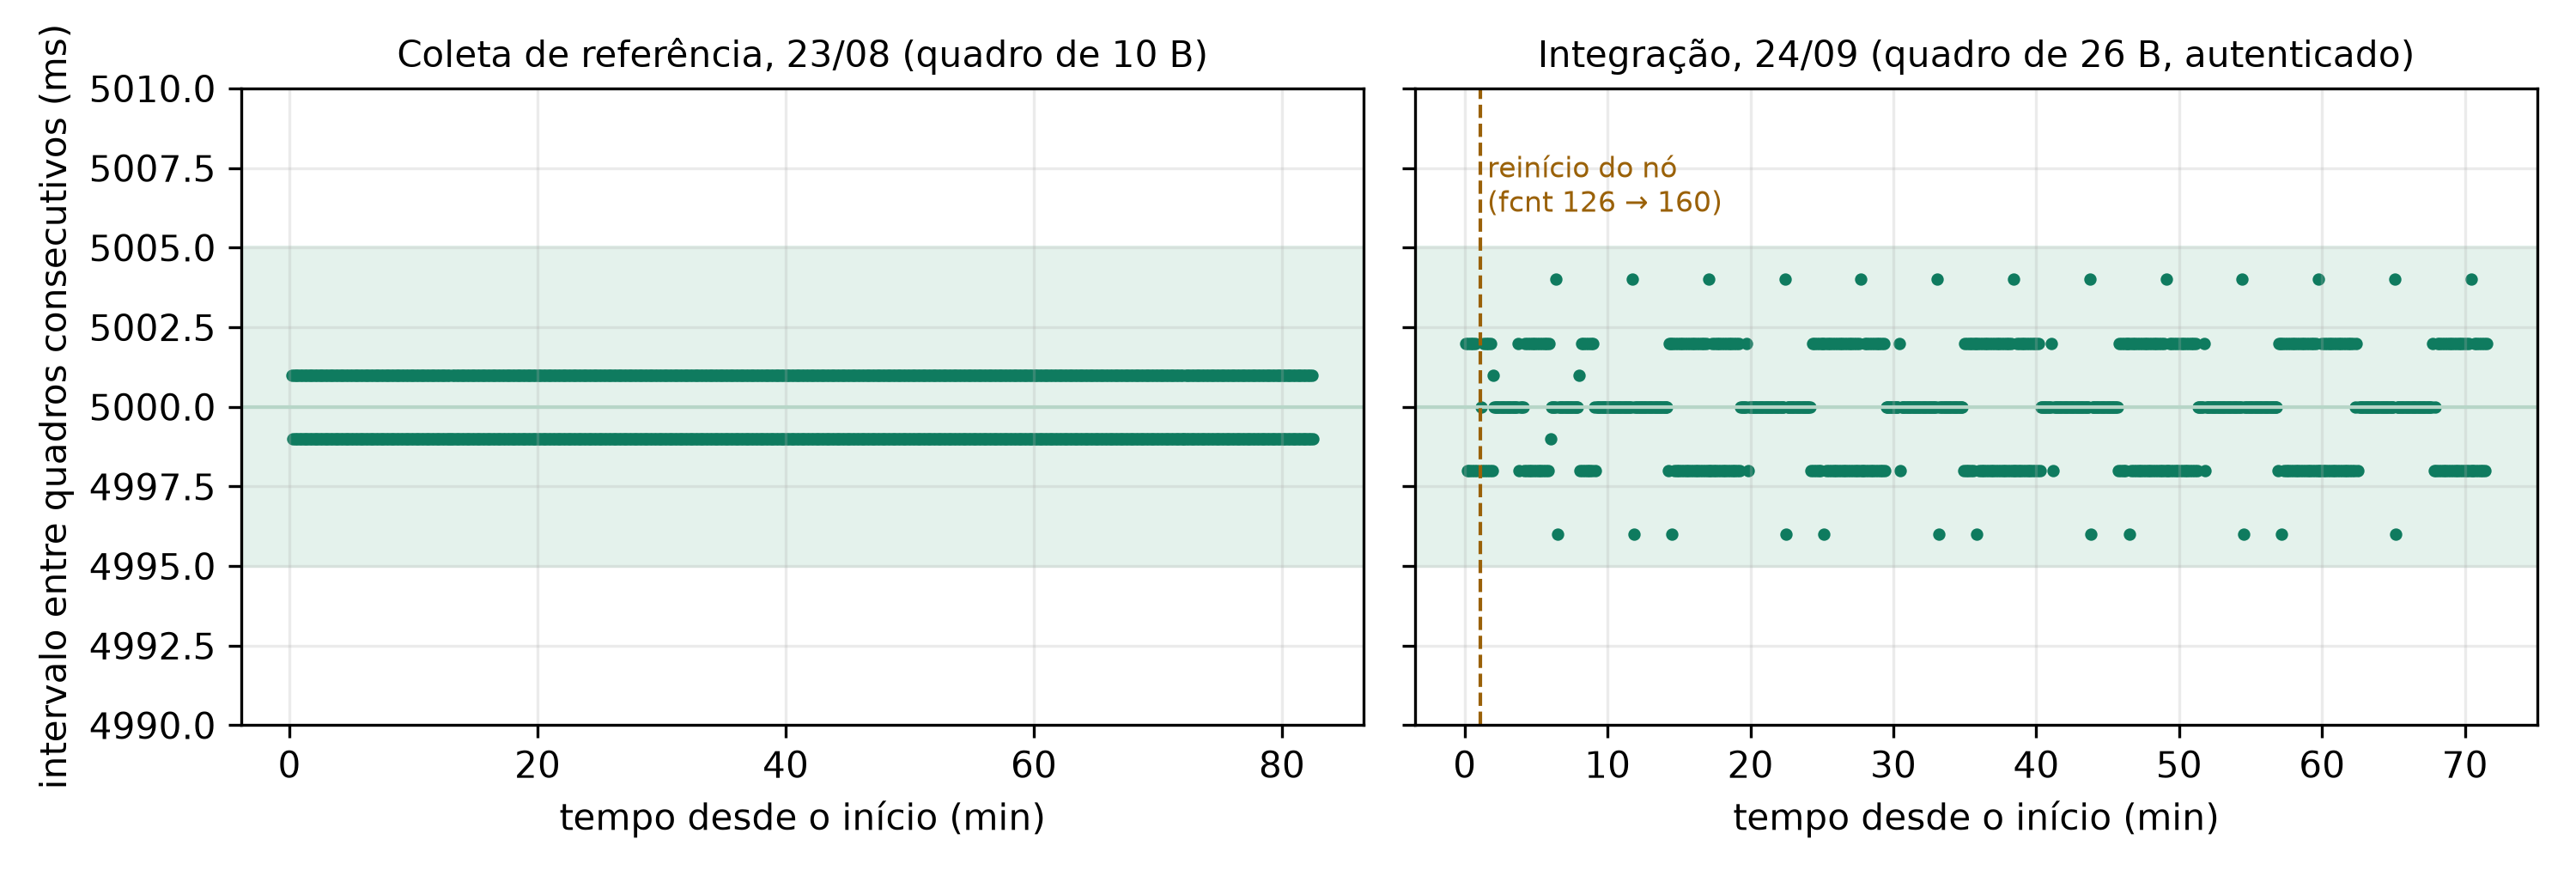
\includegraphics[width=\textwidth]{barea/figuras/cadencia_coletas.png}
  \end{center}
  \legend{Fonte: elaborado pelos autores (2026). A faixa sombreada indica $\pm 5$ ms em torno do período. A linha tracejada marca o reinício do nó.}
\end{figure}

A Figura~\ref{fig:cadencia_coletas} mostra o intervalo entre quadros consecutivos ao longo das duas coletas. Em nenhuma delas houve perda de rádio, e a cadência ficou dentro de $\pm 5$~ms do período em todos os quadros. O desvio padrão maior na segunda coleta (1,56 contra 1,00 ms) é compatível com o processamento adicional nas duas pontas, a cifragem no nó e a atividade de Wi-Fi no 	extit{gateway}, mas atribuí-lo a uma delas exigiria medição dedicada, com carimbo de tempo de microssegundo.

\begin{figure}[htb]
  \caption{\label{fig:rssi_integracao}RSSI por quadro na coleta de 24 de setembro}
  \begin{center}
      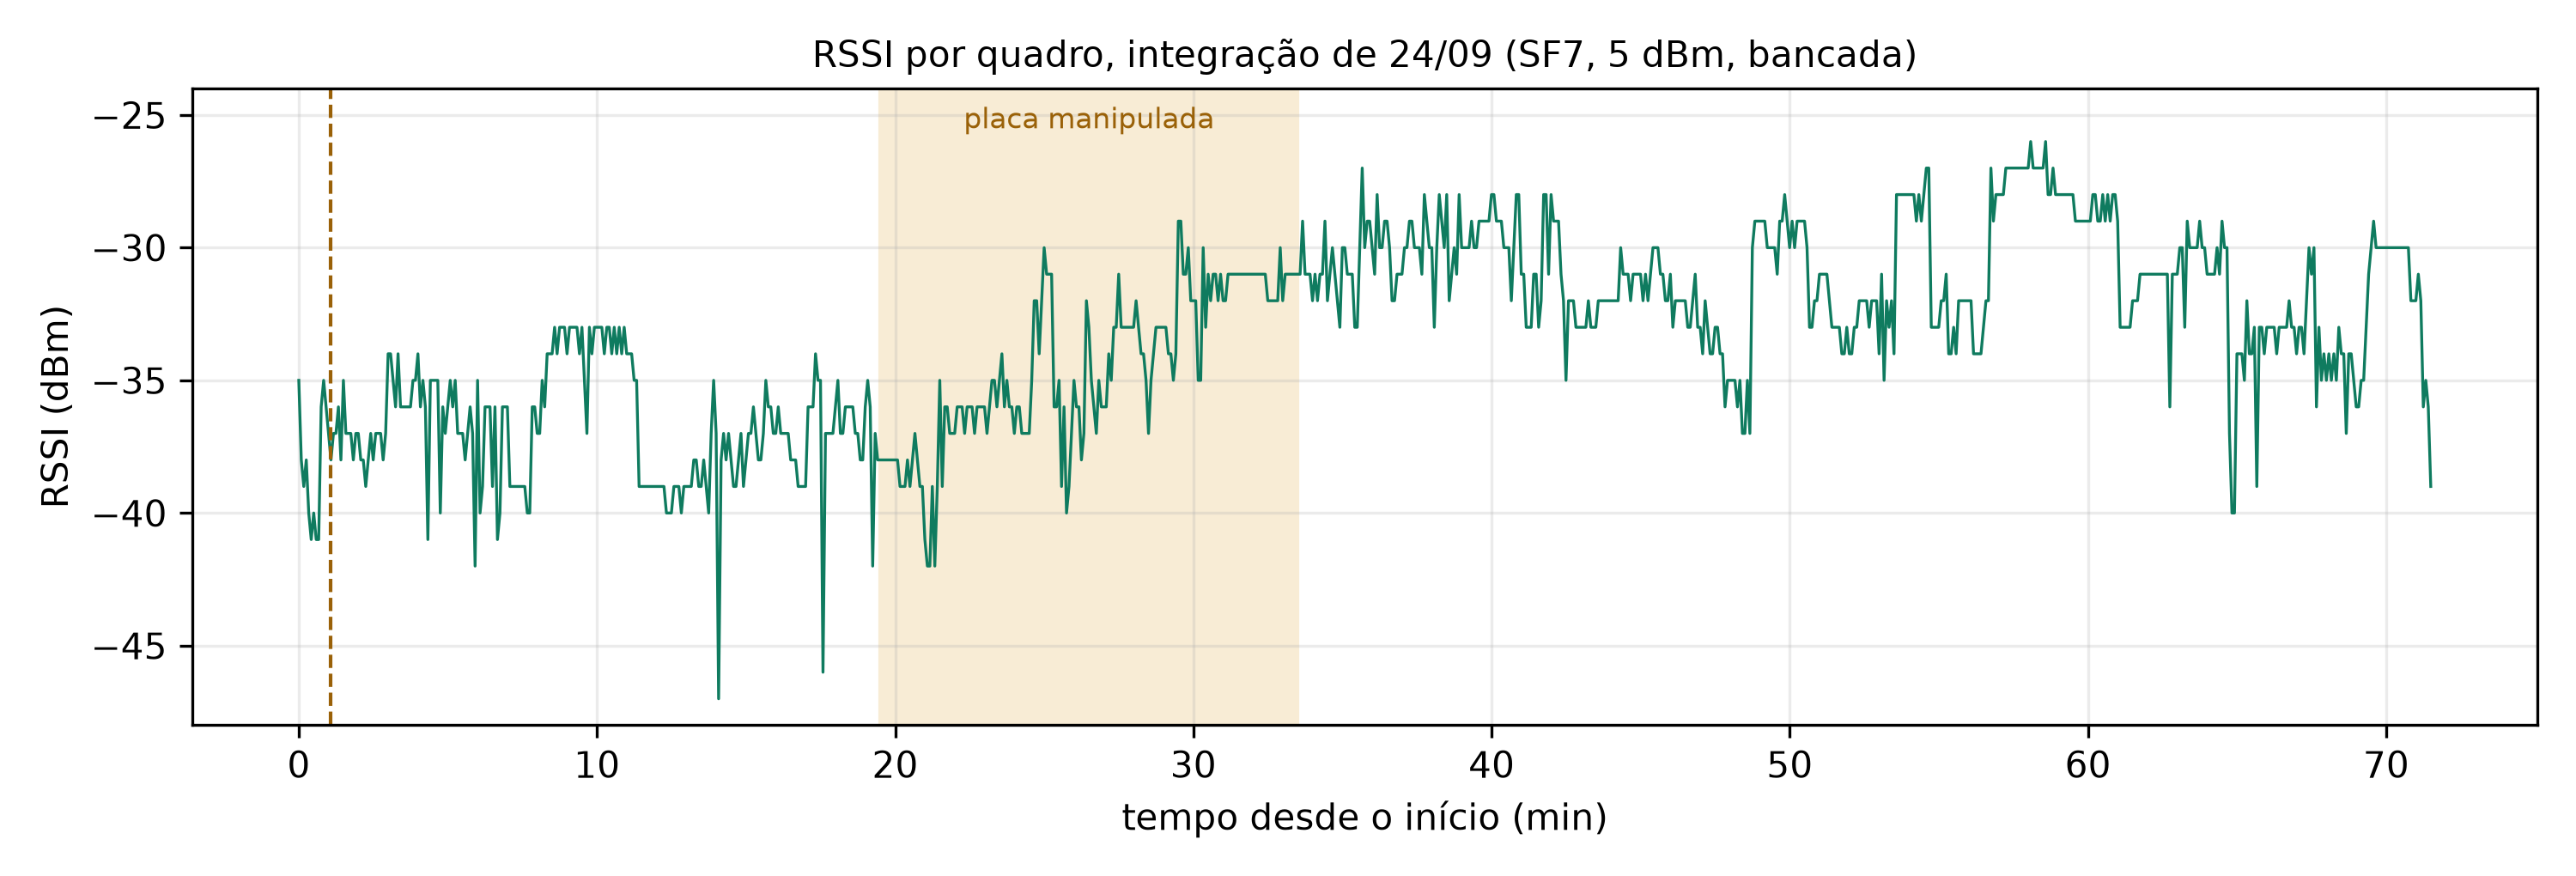
\includegraphics[width=\textwidth]{barea/figuras/rssi_integracao.png}
  \end{center}
  \legend{Fonte: elaborado pelos autores (2026). A área sombreada indica o período em que a placa do nó foi manipulada.}
\end{figure}

\subsection{Discussão}

\textbf{Reinício do nó e perda de rádio.} Na coleta de 24 de setembro, o contador saltou de 126 para 160 com intervalo de 14,7~s entre os dois quadros. Uma contagem simples registraria 33 quadros perdidos, ou 3,7\% de perda. A perda real de 33 quadros teria produzido um intervalo de cerca de 170~s; o intervalo observado e o fato de 160 ser múltiplo de 32 identificam um reinício do nó. A regra que separa os dois casos foi incorporada à API e à ferramenta de análise depois desse achado, e é o motivo de a Tabela~\ref{tab:coletas} distinguir "pulados" de "perdidos". Para a frente de aprendizado de máquina, a distinção importa: um reinício é um evento do dispositivo, uma perda é um evento do enlace, e um detector treinado sem essa separação aprenderia a confundir os dois.

\textbf{Mudança de regime no RSSI.} A Figura~\ref{fig:rssi_integracao} mostra o RSSI em torno de $-37$~dBm nos primeiros vinte minutos e entre $-30$ e $-33$~dBm a partir do trigésimo quarto, com uma transição no intervalo em que a placa do nó foi manipulada. Não é um fenômeno de rede: é a posição da antena. O episódio ilustra o que os modelos precisam distinguir: uma mudança de regime causada por intervenção física produz uma série que um detector de anomalias marcaria, e só o contexto operacional permite rotulá-la corretamente.

\textbf{SNR saturado.} Nas duas coletas o SNR variou menos de 3~dB enquanto o RSSI variou mais de 15~dB, sem correlação entre os dois. Com as placas a poucos metros, o estimador de SNR do transceptor opera saturado, como discutido na Subseção~\ref{subsec:camada_fisica_lora}. Em bancada, o SNR é uma coluna quase constante e não tem valor como variável de entrada; ele só passa a variar de forma útil em testes de alcance.

\textbf{Tempo no ar.} O tempo no ar calculado pela fórmula do fabricante para o quadro de 26 bytes em SF7 é de 61,7~ms, e para o quadro de 10 bytes, 41,2~ms. O tempo medido da função de transmissão, do início da chamada ao fim da transmissão, foi de 69 e 48~ms, respectivamente. A diferença de cerca de 7~ms é constante e corresponde ao processamento fora do rádio: montagem do quadro, cifragem e carga do transceptor. A camada de segurança acrescentou 50\% ao tempo no ar (de 41,2 para 61,7~ms), quase todo devido à tag de autenticação de 16 bytes; derivar o \textit{nonce} em vez de transmiti-lo evitou outros 16 bytes, que elevariam o tempo no ar a 87,3~ms.

\textbf{Limitações.} Uma coleta com perda zero valida a infraestrutura, mas é o caso em que nada está errado: quase toda a variabilidade que um detector precisa aprender está ausente, e as coletas apresentadas servem como referência de comportamento normal, não como conjunto de treinamento. Os dados de aplicação são sintéticos. A janela anti-replay do \textit{gateway} vive em memória volátil: um reinício do \textit{gateway} a zera, e há uma janela de repetição possível até a chegada do primeiro quadro válido, limitação que o LoRaWAN resolve persistindo o contador no \textit{network server}. Todos os nós compartilhariam uma mesma chave, ao contrário do LoRaWAN, em que cada dispositivo tem a sua. A medição de energia do nó e o teste de alcance com fatores de espalhamento maiores não foram executados.


%%%%%%%%%%%%%%%%%%%%%%%%%%%%%%%%%%%%%%%%%%%%%%%%%%%%%%
%%%%%%%%%%%%%%%%%%%%%%%%%%%%%%%%%%%%%%%%%%%%%%%%%%%%%%


\section{Resultados dos Testes da Camada de Segurança (Ascon)}
\label{sec:resultados_ascon}

Esta seção reúne os resultados dos testes de validação e avaliação da camada de segurança baseada no Ascon, seguindo a metodologia definida na Seção \ref{subsec:validacao-ascon}. A camada de segurança atua sobre o \textit{payload} de cada mensagem antes de ele ser entregue ao rádio, e os resultados a seguir não dependem da configuração do enlace, tratada na Seção~\ref{sec:resultados_infra}. As condições em que eles valem estão reunidas na Seção~\ref{subsec:limitacoes_ascon}.

%%%%%%%%%%%%%%%%%%%%%%%%%%%%%%%%%%%%%%%%%%%%%%%%%%%%%%

\subsection{Validação por \textit{Known Answer Tests} (KAT)}
\label{subsec:kat_resultados}

A validação funcional foi conduzida com os vetores oficiais do Ascon-128a (versão 1.2) distribuídos com a \textit{ascon-suite}. Inicialmente, a biblioteca foi compilada em um computador \textit{desktop} e submetida à execução exaustiva dos 1089 vetores de teste, nos quais cada combinação de chave, \textit{nonce}, dados associados e texto em claro deve produzir um texto cifrado e uma \textit{tag} de autenticação exatos.

Todos os 1089 vetores foram processados com correspondência integral em relação às saídas esperadas, sem nenhuma falha. Como verificação adicional, os vetores foram regenerados a partir da própria implementação e comparados byte a byte com o arquivo de referência, resultando em arquivos idênticos. Por fim, a suíte de testes automatizados (\textit{CTest}) foi executada sobre as variantes em C, C++, \textit{SIV} e mascarada do algoritmo, com aprovação nos 14 casos avaliados. A Tabela~\ref{tab:kat_ascon128a} sintetiza esses resultados.

\begin{table}[htb]
\centering
\caption{Resultado da validação por \textit{Known Answer Tests} do Ascon-128a}
\label{tab:kat_ascon128a}
\begin{tabular}{lrr}
\hline
\textbf{Verificação} & \textbf{Casos} & \textbf{Falhas} \\
\hline
Execução exaustiva (\textit{desktop})                  & 1089 vetores & 0 \\
Regeneração \textit{vs.} referência                    & 1089 vetores & 0 \\
Suíte \textit{CTest} (C, C++, \textit{SIV}, mascarada) & 14 testes    & 0 \\
Execução na placa (ESP32, subconjunto)                 & 6 vetores    & 0 \\
\hline
\end{tabular}
\legend{Fonte: elaborado pelos autores.}
\end{table}

Esses resultados comprovam que a implementação do Ascon-128a opera corretamente no ambiente de desenvolvimento, reproduzindo de forma exata os valores de referência do algoritmo.

Confirmada a correção em \textit{desktop}, um subconjunto representativo dos vetores foi executado diretamente na placa ESP32, cobrindo os limites de processamento por blocos, com entrada vazia, bloco parcial, bloco completo e múltiplos blocos, com e sem dados associados. Para cada vetor, verificaram-se tanto a cifragem, comparando o resultado com o valor de referência, quanto a decifragem, confirmando a recuperação do texto claro com a \textit{tag} validada. Os seis vetores foram reproduzidos com correspondência integral na placa, descartando divergências introduzidas pela compilação ou pela arquitetura do \textit{hardware} (Xtensa LX, \textit{little-endian}). Nessa execução, o estado interno do algoritmo (\texttt{ascon128a\_state\_t}) ocupou 80 bytes, valor retomado posteriormente na análise de memória.

Os vetores utilizados e o registro completo das execuções, em \textit{desktop} e na placa, estão disponíveis no repositório do projeto, na pasta \texttt{kat-validation}.

%%%%%%%%%%%%%%%%%%%%%%%%%%%%%%%%%%%%%%%%%%%%%%%%%%%%%%

\subsection{Validação dos Dados Associados (AEAD)}
\label{subsec:aead_resultados}

A propriedade de autenticação do modo AEAD foi avaliada por injeção intencional de falhas, simulando um atacante que intercepta e altera a mensagem em trânsito. A partir de um pacote válido, cada adulteração foi aplicada isoladamente e a mensagem resultante submetida à decifragem, que deveria recusá-la.

A avaliação cobriu quatro frentes de adulteração. Às três previstas na metodologia, com texto cifrado, dados associados e \textit{tag} de autenticação. Acrescentou-se o \textit{nonce}, uma vez que, em um pacote real, ele trafega em claro junto da mensagem para que o destinatário possa decifrá-la, e portanto também está ao alcance do interceptador.

Além da inversão de um bit, aplicaram-se alterações que ela não alcança, inversão de dois bits simultâneos, inversão de um byte inteiro, substituição de um byte por zero, inversão de bits em posições distantes, truncamento, acréscimo de bytes ao final e reordenação de bytes adjacentes. Todas são exaustivas e deterministas, percorrendo posições fixas do pacote sem qualquer sorteio, de modo que a bateria é integralmente reproduzível.

O procedimento foi repetido em seis formatos de pacote, escolhidos sobre as fronteiras de bloco do algoritmo, que processa 128 bits por vez, com texto claro vazio, bloco parcial, bloco exato, bloco acrescido de um byte e múltiplos blocos, com e sem dados associados. Os subtotais por formato foram 602, 476, 786, 802, 1.063 e 1.178 adulterações. A Tabela~\ref{tab:aead_ascon128a} agrega os resultados por tipo de adulteração.

\begin{table}[htb]
\centering
\caption{Rejeição de adulterações no Ascon-128a, agregada em seis formatos de pacote}
\label{tab:aead_ascon128a}
\begin{tabular}{lrr}
\hline
\textbf{Adulteração} & \textbf{Casos} & \textbf{Rejeições} \\
\hline
\multicolumn{3}{l}{\textit{Inversão de um bit}} \\
\quad Texto cifrado (\textit{ciphertext}) & 784 & 784 \\
\quad Dados associados (AD)               & 928 & 928 \\
\quad \textit{Tag} de autenticação        & 768 & 768 \\
\quad \textit{Nonce}                      & 768 & 768 \\
\multicolumn{3}{l}{\textit{Demais alterações}} \\
\quad Dois bits simultâneos               & 776 & 776 \\
\quad Byte invertido                      & 194 & 194 \\
\quad Byte substituído por zero           & 194 & 194 \\
\quad Bits em bytes distantes             &  96 &  96 \\
\quad Truncamento do pacote               & 188 & 188 \\
\quad Acréscimo de bytes                  &  24 &  24 \\
\quad Reordenação de bytes                & 187 & 187 \\
\hline
Total                                     & 4.907 & 4.907 \\
\hline
\end{tabular}
\legend{Fonte: elaborado pelos autores.}
\end{table}

Como controle, o pacote intacto foi decifrado com sucesso em todos os seis formatos, recuperando o texto claro original. Nenhuma das 4.907 adulterações foi aceita, em todas, a decifragem reconheceu a quebra de integridade e retornou erro.

A metodologia exige que nenhum fragmento do texto claro seja entregue à aplicação. Para avaliá-la, o \textit{buffer} de saída foi preenchido, antes de cada decifragem, com um valor que não ocorre no texto claro. Após cada recusa, mediu-se a maior sequência de bytes presente simultaneamente no \textit{buffer} e no texto claro original. Em todas as 4.907 recusas, essa sequência foi de zero bytes, ou seja, não restou um único byte do texto claro. O mesmo procedimento aplicado ao pacote intacto recupera a mensagem integralmente, o que confirma que a verificação detectaria um vazamento caso houvesse.

A bateria foi executada em duas plataformas, o ESP32 clássico (Xtensa LX6) e o ESP32-S3 da placa Heltec (Xtensa LX7), e os resultados foram idênticos em todos os valores. A coincidência entre arquiteturas distintas indica que a rejeição de adulterações decorre do algoritmo, e não de particularidades de uma compilação ou de um \textit{hardware}.

Qualquer alteração da mensagem em trânsito, seja no \textit{payload}, nos metadados do cabeçalho, no \textit{nonce} ou na própria \textit{tag}, é portanto detectada e rejeitada sem vazamento de conteúdo, o que satisfaz o RF-S8 e confirma o emprego da \textit{tag} em seu comprimento integral exigido pelo RNF-S5, ambos especificados na Seção~\ref{sec:requisitos_seguranca}.

Cabe registrar o limite desta propriedade. O modo AEAD garante integridade, não frescor, um pacote válido capturado e retransmitido sem alteração alguma é aceito, pois de fato não foi adulterado. A detecção de repetição exige que o receptor mantenha registro do último \textit{nonce} aceito por dispositivo e recuse valores repetidos ou regressivos, o que pertence à camada de comunicação e não ao algoritmo. Esse tratamento é objeto do RF-S9, cuja verificação não integra os resultados desta seção.

O código de teste e os registros das execuções nas duas placas estão no repositório, na pasta \texttt{aead-validation}.

%%%%%%%%%%%%%%%%%%%%%%%%%%%%%%%%%%%%%%%%%%%%%%%%%%%%%%

\subsection{Consumo de Memória, Tempo de Execução e Tempo Constante}
\label{subsec:memoria_tempo}

As medições desta seção e da seguinte foram obtidas com um único \textit{firmware} de teste, executado em duas placas, o ESP32 clássico (Xtensa LX6), usado nas etapas anteriores, e o ESP32-S3 da placa Heltec WiFi LoRa 32 V3 (Xtensa LX7), que é a plataforma de implantação. Ambas operaram a 240~MHz, com \textit{firmware} compilado pelo \textit{core} arduino-esp32 3.3.11 sobre o ESP-IDF 5.5.5. Antes de qualquer medição, ele executa dois vetores do KAT oficial do Ascon-128a e um vetor de referência do AES-GCM, cifrando, decifrando e recusando uma \textit{tag} adulterada, e uma falha interromperia a execução, como prevê a Seção~\ref{subsec:validacao-ascon}. Os tamanhos de \textit{payload} foram 0, 2, 16, 23, 32 e 64 bytes. Os múltiplos de 16 sustentam o modelo de custo por bloco, o \textit{payload} vazio mede a parcela fixa diretamente, e 2 e 23 bytes são os dois tamanhos que ocorrem no \textit{dataset} Tour Perret, usado pela frente de aprendizado de máquina, em que 91\% das mensagens têm 23 bytes e 7\% têm 2 bytes \cite{tourperret_dataset}. O \textit{firmware}, os registros das duas placas e o programa que gera as tabelas e figuras estão na pasta \texttt{benchmark-validation/Ascon128a\_Benchmark\_Suite} do repositório.

Quanto à memória, a cifragem e a decifragem do Ascon-128a não realizaram nenhuma alocação dinâmica em nenhum dos seis tamanhos, nas duas placas. Como uma alocação feita e liberada dentro da operação não apareceria numa comparação antes e depois, o \textit{heap} livre foi lido continuamente durante cada operação por uma tarefa no outro núcleo do processador, e o menor valor observado coincidiu com o inicial em todos os casos. O mesmo procedimento aplicado ao AES-128-GCM mostrou que, no ESP32-S3, o \textit{driver} do ESP-IDF aloca e libera 40 bytes a cada chamada, por causa dos descritores da transferência por DMA \cite{espressif2026idf}. No ESP32 clássico, cujo \textit{driver} não usa DMA, não houve alocação. O resultado atende ao RNF-S6 para o Ascon e mostra que a mesma afirmação não vale para o AES na placa de implantação. O estado interno do algoritmo ocupa 80 bytes e os \textit{buffers} de entrada e saída têm tamanho fixo, de modo que o consumo de memória não depende do \textit{payload}, como exige o RNF-S7.

A profundidade de pilha foi medida numa tarefa criada só para isso, pela marca d'água da pilha antes e depois de oito execuções com 64 bytes. A cifragem do Ascon-128a consumiu 340 bytes de pilha no ESP32 clássico e 224 no ESP32-S3, e a decifragem, 436 bytes em ambos. O AES-128-GCM consumiu 548 e 628 bytes (cifragem e decifragem) no ESP32 clássico, e 628 e 804 no ESP32-S3. Em relação à memória de programa (\textit{Flash}), mediu-se o custo da biblioteca com um \textit{firmware} mínimo que cifra e decifra 16 bytes, compilado duas vezes, uma com as chamadas à biblioteca e outra sem elas, de modo que a diferença entre os dois binários é o código da biblioteca. A diferença foi de 6.800 bytes no ESP32 clássico (277.744 bytes contra 270.944), o equivalente a 0,5\% da partição de aplicação de 1.310.720 bytes, e de 6.812 bytes no ESP32-S3 (282.257 contra 275.445), 0,2\% de sua partição de 3.342.336 bytes.

O tempo de execução foi obtido lendo o contador de ciclos da CPU imediatamente antes e depois de cada chamada. Em cada tamanho e operação tomou-se o piso, o menor valor de 2.000 medidas, com as interrupções habilitadas, e o procedimento foi repetido em 100 execuções independentes. O piso foi idêntico nas 100 execuções em todos os tamanhos e operações, nas duas placas. Medindo-se também a cifragem com as interrupções desabilitadas, o piso coincidiu com o das interrupções habilitadas a menos de 2 ciclos, o que confirma que as interrupções não o afetam. O desvio padrão das medidas dentro de cada execução, entre 140 e 230 ciclos com as interrupções habilitadas, é justamente o ruído que o piso elimina. A Tabela~\ref{tab:tempo_ascon128a} apresenta os pisos.

\begin{table}[htb]
\centering
\caption{Piso de ciclos do Ascon-128a por tamanho de \textit{payload}, cifragem e decifragem, nas duas placas (100 execuções de 2.000 medidas cada, dispersão nula entre execuções)}
\label{tab:tempo_ascon128a}
\begin{tabular}{rrrrr}
\hline
\textbf{\textit{Payload}} & \multicolumn{2}{c}{\textbf{ESP32 clássico}} & \multicolumn{2}{c}{\textbf{ESP32-S3}} \\
 & \textbf{cifragem} & \textbf{decifragem} & \textbf{cifragem} & \textbf{decifragem} \\
\hline
0 bytes  & 5.037 & 5.256  & 4.603 & 4.755 \\
2 bytes  & 5.181 & 5.366  & 4.722 & 4.841 \\
16 bytes & 6.134 & 6.646  & 5.639 & 5.959 \\
23 bytes & 6.521 & 6.989  & 5.960 & 6.212 \\
32 bytes & 7.231 & 8.036  & 6.675 & 7.163 \\
64 bytes & 9.425 & 10.816 & 8.747 & 9.571 \\
\hline
\end{tabular}
\legend{Fonte: elaborado pelos autores.}
\end{table}

O custo é linear no número de blocos completos de 16 bytes, no ESP32 clássico, 5.037 ciclos fixos mais 1.097 por bloco na cifragem, e 5.256 mais 1.390 na decifragem. No ESP32-S3, 4.603 mais 1.036, e 4.755 mais 1.204. O ponto de 32 bytes cai exatamente sobre a reta definida por 16 e 64 bytes, e a parcela fixa medida com o \textit{payload} vazio coincidiu com a extrapolada. A decifragem custa mais que a cifragem, e parte da diferença vem da verificação da \textit{tag}, que na biblioteca percorre o texto claro inteiro para apagá-lo em caso de falha, um custo proporcional ao tamanho da mensagem \cite{weatherley2023ascon}.

Os tamanhos intermediários seguem a especificação do algoritmo, a permutação é aplicada após cada bloco de texto claro exceto o último, que é apenas preenchido \cite{ascon_v12_spec}. Assim, em número de permutações, 2 bytes equivalem a 0 e 23 equivalem a 16. O acréscimo medido em relação a essa previsão (144 ciclos de 0 para 2 bytes e 387 de 16 para 23, no ESP32 clássico) corresponde ao tratamento byte a byte dos bytes que não completam um bloco \cite{weatherley2023ascon}, de 46 a 72 ciclos por byte. A mensagem típica de 23 bytes custa 6.521 ciclos (27,2~$\mu$s) no ESP32 clássico e 5.960 ciclos (24,8~$\mu$s) no ESP32-S3, 6\% acima de 16 bytes e 10\% abaixo de 32. A primeira chamada de cada função após a ativação, com a \textit{cache} de instruções ainda vazia, custou 53.314 ciclos (222~$\mu$s) na cifragem do ESP32 clássico e 52.127 (217~$\mu$s) no ESP32-S3, cerca de nove vezes o piso. É o custo de carregar o código da \textit{Flash}, pago uma vez, e não do algoritmo. Mesmo esse valor é desprezível frente ao tempo de transmissão. Tomando como exemplo um enlace com fator de espalhamento 7, largura de banda de 125~kHz, taxa de código 4/5, cabeçalho explícito e CRC, a fórmula de tempo no ar do rádio LoRa \cite{semtech2015sx1276} dá cerca de 87~ms para um pacote de 43 bytes (23 de \textit{payload} mais os 20 bytes de contador e \textit{tag} da Seção~\ref{subsec:asconsecure}). É mais de três mil vezes o tempo da cifragem, e mais de trezentas vezes o da primeira chamada, o que atende ao RNF-S8. O valor é calculado pela fórmula do fabricante, não medido.

Por fim, avaliou-se a resistência a ataques de canal colateral baseados em tempo. Além da variação de chave e conteúdo ao longo das 2.000 medidas, prevista na metodologia, a cifragem foi medida com cinco classes de entrada, com as interrupções desabilitadas. As classes são a rampa usada nas demais medições, chave e texto todos nulos, todos 0xFF, alternados entre 0x55 e 0xAA, e bytes derivados de um \textit{hash}. A comparação entre classes fixas e variáveis segue o princípio do método dudect \cite{reparaz2017dudect}. O piso foi idêntico nas cinco classes em ambas as placas, com 6.135 e 9.426 ciclos no ESP32 clássico para 16 e 64 bytes, e 5.639 e 8.747 no ESP32-S3. As médias diferiram entre classes em no máximo 0,02 ciclo no ESP32 clássico e 0,41 ciclo no ESP32-S3, sobre milhares de ciclos (Figura~\ref{fig:bench_tempo_constante}). No ESP32-S3 as medidas individuais tiveram desvio padrão de cerca de 25 ciclos mesmo sem interrupções, contra menos de 0,5 no ESP32 clássico, sem relação com a classe de entrada. Esses resultados corroboram a propriedade de tempo constante do Ascon, decorrente de sua camada de substituição sem tabelas de consulta \cite{ascon_v12_spec}, e atendem ao RNF-S9.

\begin{figure}[htb]
  \caption{\label{fig:bench_tempo_constante}Tempo constante. Diferença entre a média e o piso de 2.000 cifragens, por classe de entrada, em 16 e 64 bytes, nas duas placas}
  \begin{center}
      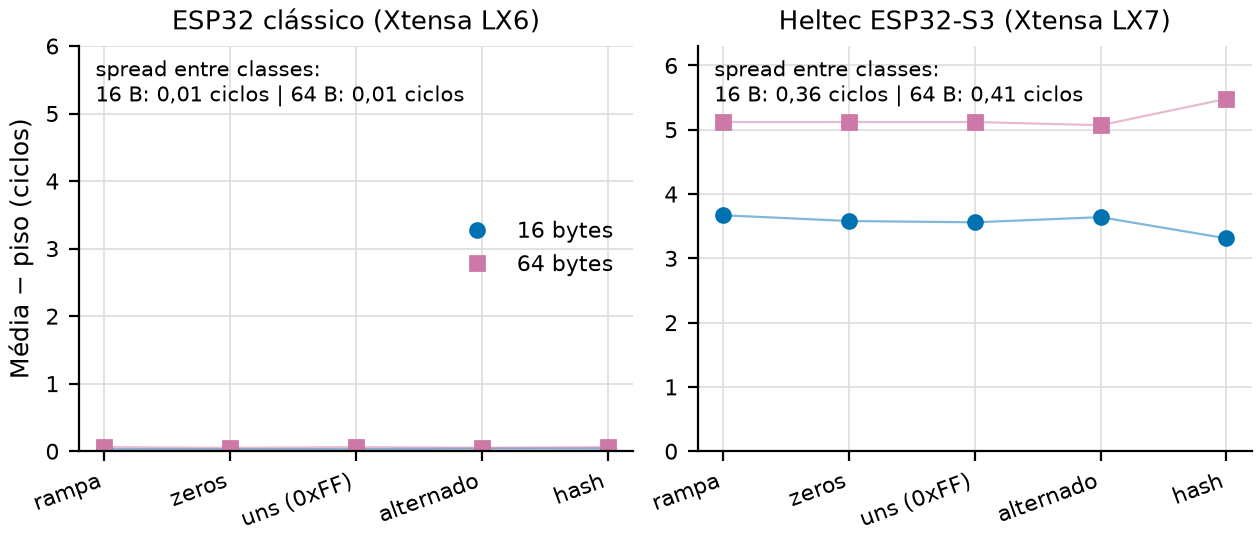
\includegraphics[width=\textwidth]{felipe/figuras/bench_tempo_constante.png}
  \end{center}
  \legend{Fonte: elaborado pelos autores.}
\end{figure}

%%%%%%%%%%%%%%%%%%%%%%%%%%%%%%%%%%%%%%%%%%%%%%%%%%%%%%

\subsection{Comparativo com AES-128-GCM}
\label{subsec:comparativo_aes}

Para responder à questão central levantada na Seção 2.2.2, se a migração para criptografia leve em \textit{software} traz vantagem real frente ao acelerador de \textit{hardware} já presente nas placas comerciais, comparou-se o Ascon-128a (\textit{software}) com o AES-128-GCM (\textit{Galois/Counter Mode}) na mesma execução e sob as mesmas condições, nas duas placas. O AES-GCM foi avaliado por meio da biblioteca \textit{mbedTLS} do próprio \textit{core} do ESP32, com a chave fixada uma vez por execução, como num nó que possui uma única chave. Nos dois chips, apenas o bloco AES é executado no acelerador de \textit{hardware}. A autenticação (GHASH) permanece em \textit{software}, e nenhum dos dois declara suporte a GCM no acelerador \cite{espressif2026idf}. As placas diferem no caminho pelo qual o \textit{driver} alimenta o acelerador. No ESP32 clássico a CPU escreve e lê um bloco de 16 bytes por vez, e no ESP32-S3 o \textit{driver} usa DMA \cite{espressif2026idf}.

Cada algoritmo foi medido pelo piso de 2.000 medidas, alternando-se os dois na mesma execução, em 100 execuções por tamanho, para cifragem e decifragem. A Tabela~\ref{tab:comparativo_aes} apresenta os pisos da cifragem e a razão entre eles, e a Tabela~\ref{tab:comparativo_aes_dec} faz o mesmo para a decifragem. A decifragem interessa por conta própria, pois é a operação que o receptor executa para cada pacote de cada nó. A Figura~\ref{fig:bench_ciclos_tamanho} mostra as mesmas curvas, com a cifragem acima e a decifragem abaixo.

\begin{table}[htb]
\centering
\caption{Piso de ciclos da cifragem do Ascon-128a (\textit{software}) e do AES-128-GCM (\textit{mbedTLS}), nas duas placas, e razão AES/Ascon}
\label{tab:comparativo_aes}
\begin{tabular}{rrrrrrr}
\hline
\textbf{\textit{Payload}} & \multicolumn{3}{c}{\textbf{ESP32 clássico}} & \multicolumn{3}{c}{\textbf{ESP32-S3}} \\
 & \textbf{Ascon} & \textbf{AES-GCM} & \textbf{razão} & \textbf{Ascon} & \textbf{AES-GCM} & \textbf{razão} \\
\hline
0 bytes  & 5.037 & 6.497  & 1,29 & 4.603 & 10.465 & 2,27 \\
2 bytes  & 5.181 & 8.174  & 1,58 & 4.722 & 16.556 & 3,51 \\
16 bytes & 6.134 & 8.603  & 1,40 & 5.639 & 19.473 & 3,45 \\
23 bytes & 6.521 & 10.454 & 1,60 & 5.960 & 20.920 & 3,51 \\
32 bytes & 7.231 & 10.712 & 1,48 & 6.675 & 20.398 & 3,06 \\
64 bytes & 9.425 & 14.930 & 1,58 & 8.747 & 22.267 & 2,55 \\
\hline
\end{tabular}
\legend{Fonte: elaborado pelos autores.}
\end{table}

\begin{table}[htb]
\centering
\caption{Piso de ciclos da decifragem do Ascon-128a (\textit{software}) e do AES-128-GCM (\textit{mbedTLS}), nas duas placas, e razão AES/Ascon}
\label{tab:comparativo_aes_dec}
\begin{tabular}{rrrrrrr}
\hline
\textbf{\textit{Payload}} & \multicolumn{3}{c}{\textbf{ESP32 clássico}} & \multicolumn{3}{c}{\textbf{ESP32-S3}} \\
 & \textbf{Ascon} & \textbf{AES-GCM} & \textbf{razão} & \textbf{Ascon} & \textbf{AES-GCM} & \textbf{razão} \\
\hline
0 bytes  & 5.256  & 6.908  & 1,31 & 4.755 & 10.814 & 2,27 \\
2 bytes  & 5.366  & 8.585  & 1,60 & 4.841 & 16.903 & 3,49 \\
16 bytes & 6.646  & 9.014  & 1,36 & 5.959 & 19.820 & 3,33 \\
23 bytes & 6.989  & 10.867 & 1,55 & 6.212 & 21.269 & 3,42 \\
32 bytes & 8.036  & 11.123 & 1,38 & 7.163 & 20.745 & 2,90 \\
64 bytes & 10.816 & 15.341 & 1,42 & 9.571 & 22.616 & 2,36 \\
\hline
\end{tabular}
\legend{Fonte: elaborado pelos autores.}
\end{table}

\begin{figure}[htb]
  \caption{\label{fig:bench_ciclos_tamanho}Piso de ciclos da cifragem (acima) e da decifragem (abaixo) por tamanho de \textit{payload}, Ascon-128a e AES-128-GCM, nas duas placas}
  \begin{center}
      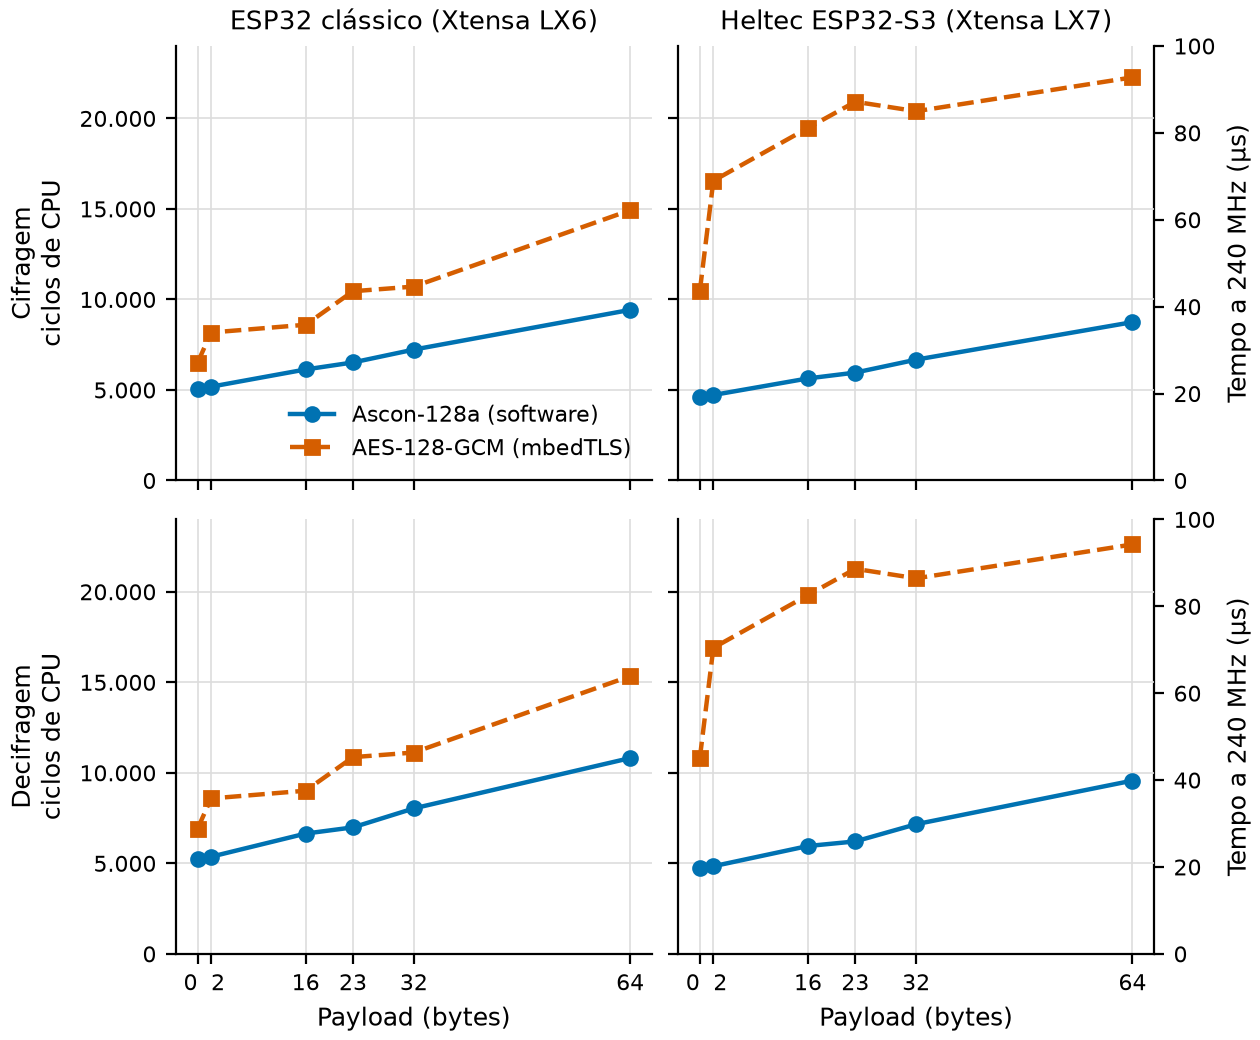
\includegraphics[width=\textwidth]{felipe/figuras/bench_ciclos_tamanho.png}
  \end{center}
  \legend{Fonte: elaborado pelos autores.}
\end{figure}

O Ascon-128a foi mais rápido que o AES-128-GCM em todas as 1.200 execuções de cada placa (seis tamanhos, cifragem e decifragem, 100 execuções). No ESP32 clássico a vantagem vai de 1,29 vez, com o \textit{payload} vazio, a 1,60 vez, em 23 bytes, e tende a crescer com o número de blocos. Na decifragem, vai de 1,31 a 1,60. No ESP32-S3 ela vai de 2,27 a 3,51 vezes na cifragem e de 2,27 a 3,49 na decifragem, e diminui com o tamanho (Figura~\ref{fig:bench_razao_tamanho}). As duas tendências têm a mesma origem, o custo por bloco e a parcela fixa de cada caminho do AES, examinados a seguir.

\begin{figure}[htb]
  \caption{\label{fig:bench_razao_tamanho}Razão entre os pisos de ciclos do AES-128-GCM e do Ascon-128a, na cifragem e na decifragem, por tamanho de \textit{payload}}
  \begin{center}
      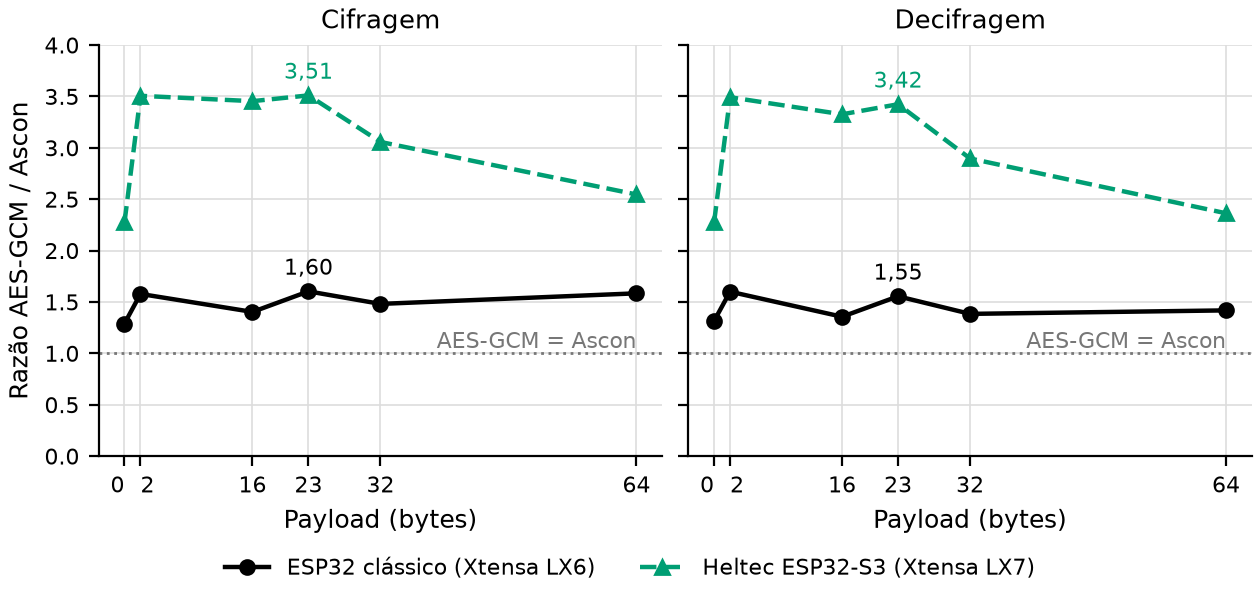
\includegraphics[width=\textwidth]{felipe/figuras/bench_razao_tamanho.png}
  \end{center}
  \legend{Fonte: elaborado pelos autores.}
\end{figure}

O AES-GCM é a cifragem em modo contador (CTR) mais o cálculo da \textit{tag} pelo GHASH \cite{dworkin2007gcm}, e no ESP-IDF a rotina de GCM reutiliza a de CTR \cite{espressif2026idf}. Assim, a diferença entre os custos por bloco dos dois modos é o GHASH, e por isso mediu-se também o AES-128-CTR. Ele entra aqui só como instrumento de medição, pois sem autenticação não atenderia ao requisito desta camada. A Figura~\ref{fig:bench_decomposicao_bloco} resume a decomposição. No ESP32 clássico, cada bloco adicional de 16 bytes custa 825 ciclos no AES-CTR e 2.109 no AES-GCM, logo 1.284 ciclos no GHASH. No ESP32-S3, são 49 ciclos no CTR, 931 no GCM e 882 no GHASH. Em ambos, o GHASH sozinho custa mais do que o Ascon-128a gasta para cifrar e autenticar um bloco inteiro (1.097 e 1.036 ciclos). Mesmo os 825 ciclos por bloco do CTR no ESP32 clássico estão longe do núcleo do acelerador, ao qual o manual do fabricante atribui 11 a 15 ciclos de \textit{clock} por bloco \cite{espressif2026trm}. O restante é gasto pelo \textit{software} do \textit{driver} e pela transferência dos dados entre a CPU e o periférico.

\begin{figure}[htb]
  \caption{\label{fig:bench_decomposicao_bloco}Custo marginal por bloco de 16 bytes do Ascon-128a completo e do AES-128-GCM decomposto em cifra AES (CTR) e GHASH, nas duas placas}
  \begin{center}
      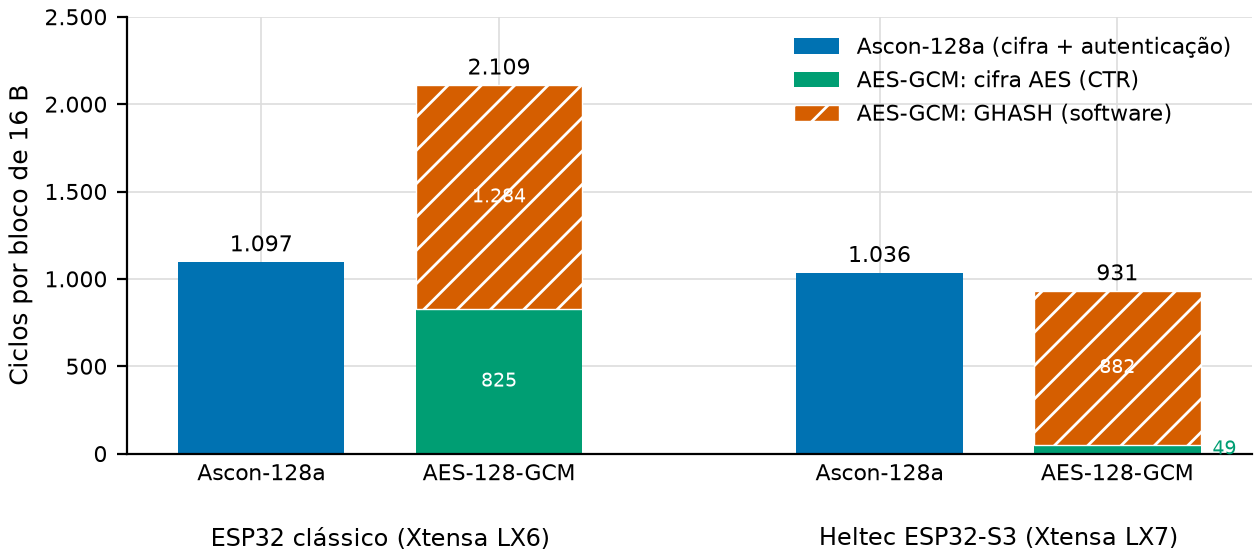
\includegraphics[width=\textwidth]{felipe/figuras/bench_decomposicao_bloco.png}
  \end{center}
  \legend{Fonte: elaborado pelos autores.}
\end{figure}

No ESP32-S3, o caminho por DMA reduz o custo por bloco a 49 ciclos, mas cobra caro por chamada. Cada transferência exige preparar e depois liberar o canal de DMA \cite{espressif2026idf}, e o AES-CTR de 16 bytes custou 8.218 ciclos, contra 2.316 no ESP32 clássico. Como o GCM faz duas transferências por mensagem, uma para os dados e outra para a \textit{tag}, sua parcela fixa chega a cerca de 18.500 ciclos, e é isso que torna o AES-GCM 3,5 vezes mais lento que o Ascon na mensagem de 23 bytes. O bloco parcial recebe tratamento à parte no \textit{driver}, o que ajuda a explicar 23 bytes terem custado mais que 32 (20.920 contra 20.398 ciclos). Os pisos do AES-GCM no ESP32-S3 variaram até 8 ciclos entre as 100 execuções, cerca de 0,04\%, e no ESP32 clássico no máximo 2. Os do Ascon não variaram em nenhum caso.

Para os pacotes pequenos típicos de redes LoRaWAN, portanto, a criptografia leve em \textit{software} não apenas dispensa o acelerador de \textit{hardware} como o supera em latência nos dois chips, e por margem maior justamente na placa de implantação, mantendo ainda a ausência de alocação dinâmica, que o AES não mantém no ESP32-S3. Ressalva-se que o resultado se refere ao AES-GCM do \textit{mbedTLS} pelo \textit{port} da Espressif, nas versões indicadas. Entre os alvos do ESP-IDF, apenas o ESP32-S2 declara aceleração de GCM, e ainda assim parcial, pois o GHASH permanece em \textit{software}, de modo que não se espera que a comparação se inverta nas demais variantes \cite{espressif2026idf}. O consumo energético dessa mesma comparação é apresentado na Seção~\ref{subsec:energia_resultados}.

%%%%%%%%%%%%%%%%%%%%%%%%%%%%%%%%%%%%%%%%%%%%%%%%%%%%%%

\subsection{Consumo Energético}
\label{subsec:energia_resultados}

A energia por operação foi medida pelo procedimento da Seção~\ref{subsec:energia_metodo}, nas duas placas, com a mensagem de 23 bytes. Um \textit{firmware} próprio, que executa um autoteste antes de começar, repetiu cada operação 20.000 vezes por rajada. Os cinco casos foram a cifragem e a decifragem do Ascon-128a e do AES-128-GCM e o controle, em que o processador apenas aguarda 27~$\mu$s por repetição. O resistor foi de 1~$\Omega$, com tolerância de 1\%. A tensão na placa foi medida com multímetro no ESP32-S3, 3,2~V, e não foi medida no ESP32 clássico, para o qual se adotou 3,25~V. O \textit{firmware}, as leituras e as capturas de tela do osciloscópio estão na pasta \texttt{benchmark-validation/Ascon128a\_Energy\_Burst} do repositório.

No ESP32 clássico, a média da rajada e a do repouso foram lidas na mesma captura, como previsto. No ESP32-S3, o osciloscópio calculou a média entre cursores apenas no instante da captura, e as duas médias vieram de capturas distintas, com os cursores fixados antes do disparo. Como o repouso é o mesmo estado da placa em todos os casos, adotou-se para cada placa um único valor, a média das cinco leituras de repouso, 49,0~mV no ESP32 clássico e 43,1~mV no ESP32-S3. Essas leituras variaram de 48,0 a 52,1~mV na primeira placa e de 42,0 a 46,2~mV na segunda, com desvio padrão de 1,7 e 1,8~mV. O acréscimo de corrente tem, portanto, incerteza de cerca de 2~mA, entre 7\% e 9\% do valor nos quatro casos com algoritmo. A Tabela~\ref{tab:energia_ascon128a} apresenta os resultados.

\begin{table}[htb]
\centering
\caption{Duração da rajada de 20.000 operações, acréscimo de corrente sobre o repouso e energia por operação, com mensagem de 23 bytes, nas duas placas}
\label{tab:energia_ascon128a}
\begin{tabular}{lrrrrrr}
\hline
\textbf{Caso} & \multicolumn{3}{c}{\textbf{ESP32 clássico}} & \multicolumn{3}{c}{\textbf{ESP32-S3}} \\
 & \textbf{s} & \textbf{mA} & \textbf{$\mu$J} & \textbf{s} & \textbf{mA} & \textbf{$\mu$J} \\
\hline
Controle                 & 0,55 & 12,6 & 1,1 & 0,556 & 19,8 & 1,8 \\
Ascon-128a, cifragem     & 0,52 & 25,1 & 2,1 & 0,499 & 28,1 & 2,2 \\
Ascon-128a, decifragem   & 0,57 & 25,6 & 2,4 & 0,520 & 27,9 & 2,3 \\
AES-128-GCM, cifragem    & 1,02 & 22,4 & 3,7 & 1,756 & 27,9 & 7,8 \\
AES-128-GCM, decifragem  & 1,05 & 22,5 & 3,8 & 1,786 & 25,9 & 7,4 \\
\hline
\end{tabular}
\legend{Fonte: elaborado pelos autores.}
\end{table}

O Ascon-128a gastou entre 2,1 e 2,4~$\mu$J por operação, nas duas placas. O AES-128-GCM gastou 3,7 e 3,8~$\mu$J no ESP32 clássico, 1,8 e 1,6 vez a energia do Ascon na cifragem e na decifragem, e 7,8 e 7,4~$\mu$J no ESP32-S3, 3,5 e 3,2 vezes. Essas razões carregam a incerteza de cada medida.

A diferença vem do tempo, e não da potência. Durante a rajada os dois algoritmos acrescentaram correntes próximas, de 22 a 28~mA, e no ESP32-S3 praticamente iguais na cifragem, 28,1 e 27,9~mA. O que muda é a duração. No ESP32-S3 cada operação do AES-128-GCM durou 87,8~$\mu$s e cada operação do Ascon-128a, 24,9~$\mu$s, a mesma razão de 3,5 vezes medida em ciclos na Tabela~\ref{tab:comparativo_aes}, cuja origem é a parcela fixa do caminho por DMA discutida na Seção~\ref{subsec:comparativo_aes}. O caso de controle mostra que manter o núcleo ocupado, sem algoritmo algum, já acrescenta 12,6~mA no ESP32 clássico e 19,8~mA no ESP32-S3. O Ascon acrescenta a isso cerca de 13~mA na primeira placa e 8~mA na segunda.

As durações das rajadas foram comparadas com os pisos de ciclos das seções anteriores, multiplicados pelas 20.000 repetições. No ESP32-S3, em que a duração foi medida pelo próprio osciloscópio, as quatro ficaram a menos de 1\% do previsto, com 0,499~s contra 0,497~s na cifragem do Ascon e 1,756~s contra 1,743~s na do AES-GCM. No ESP32 clássico, em que foi lida pelos cursores com resolução de 0,03~s, as do Ascon ficaram dentro dessa margem. As do AES-GCM duraram 1,02 e 1,05~s, contra 0,87 e 0,91~s previstos. A causa dessa diferença não foi investigada, e a energia foi calculada com a duração medida.

%%%%%%%%%%%%%%%%%%%%%%%%%%%%%%%%%%%%%%%%%%%%%%%%%%%%%%

\subsection{Integração no enlace LoRa: biblioteca \textit{AsconSecure}}
\label{subsec:asconsecure}

As seções anteriores validam o algoritmo. Para que a frente de comunicação o utilize sem lidar com chave, \textit{nonce} ou contador, a camada de segurança foi empacotada como uma biblioteca Arduino, a \textit{AsconSecure}, na pasta \texttt{ascon-lora} do repositório. Ela reúne três papéis. O provisionamento do nó é feito uma vez na bancada, o emissor cifra no nó sensor, e o receptor decifra no \textit{gateway}. Para a aplicação, o uso se resume a uma chamada para cifrar e uma para decifrar. Quando a operação falha, o resultado não contém bytes, e não há o que transmitir ou consumir.

Cada mensagem no ar é formada por um contador de 4 bytes, pelo texto cifrado e pela \textit{tag} de 16 bytes, o que acrescenta 20 bytes fixos ao \textit{payload}. O \textit{nonce} de 128 bits é composto por um prefixo de 12 bytes, gerado no provisionamento e conhecido pelo receptor, seguido do contador, e só o contador viaja. Ele não precisa de proteção à parte, pois alterá-lo em trânsito altera o \textit{nonce} e invalida a \textit{tag}, como mostrou a Seção~\ref{subsec:aead_resultados}.

A chave de 128 bits e o prefixo são gerados no próprio nó, pelo CTR\_DRBG da \textit{mbedTLS} alimentado pelo gerador de \textit{hardware} do ESP32 (RF-S3 e RF-S4), e gravados na memória não volátil (NVS). A saída do gerador é usada diretamente como chave, o caso $V$ nulo da operação $K = U \oplus V$ do SP 800-133r2 \cite{barker2020nist133}. Um cuidado vem da documentação do ESP-IDF. O gerador de \textit{hardware} só produz números verdadeiramente aleatórios com o Wi-Fi ou o Bluetooth ligados, ou com uma fonte interna de entropia habilitada por \texttt{bootloader\_random\_enable()}, e fora dessas condições sua saída deve ser considerada apenas pseudoaleatória \cite{espressif2026random}. Como o nó não usa Wi-Fi nem Bluetooth, a biblioteca habilita essa fonte durante a geração da chave e a desabilita em seguida. A mesma documentação exige que isso ocorra antes de o conversor analógico-digital ou o rádio serem iniciados, e por isso a geração da chave é uma etapa própria, o provisionamento, separada da inicialização do emissor. Como cada nó gera a própria chave, nenhuma é compartilhada (RF-S6), e o \textit{gateway} não tem chave própria, apenas guarda a de cada nó que escuta.

A unicidade do \textit{nonce} (RNF-S2 e RF-S7) vem de um contador de 32 bits persistido na NVS. Para não gravar a \textit{flash} a cada mensagem, o emissor reserva 32 valores por vez, gravando o valor 32 posições à frente antes de usar a faixa, e só volta a gravar quando ela se esgota. Após uma reinicialização, o contador recomeça do valor reservado, pois tudo abaixo dele pode ter ido ao ar. Uma queda de energia descarta até 32 valores, mas nunca repete um, e diante de $2^{32}$ valores o descarte é irrelevante. O contador pertence a esta camada e independe do contador de quadros do LoRaWAN, como exige o RF-S7. Perto do fim, a cifragem é recusada antes que o valor dê a volta, e a saída é reprovisionar o nó.

No \textit{gateway}, o receptor guarda na NVS, para cada nó, o maior contador já aceito. A decifragem verifica primeiro a \textit{tag} e depois o contador. Um pacote com \textit{tag} inválida é descartado antes de qualquer consulta ao estado, para que um pacote forjado com contador alto não bloqueie o nó legítimo, e um pacote autêntico com contador igual ou menor que o último aceito é descartado como repetição (RF-S9). O novo contador é gravado antes de a mensagem ser entregue. Se a gravação falhar, a mensagem é descartada, pois entregar sem gravar permitiria, após um reinício, aceitar de novo tudo o que chegou no intervalo. O texto claro fica num \textit{buffer} interno e só é copiado à aplicação depois das duas verificações, o que estende ao código de integração a garantia do RF-S8. O registro é indexado por uma impressão da chave, os 8 primeiros bytes do \textit{hash} Ascon de chave e prefixo, e não pelo número do nó, para que um erro de configuração, como registrar o mesmo nó sob dois números, não reabra o histórico à repetição.

A renovação da chave (RF-S5) é feita por novo provisionamento, em que se apaga o estado do nó, gera-se nele uma chave nova e substitui-se o registro no receptor. Nenhuma chave trafega pelo ar.

Os \textit{buffers} da biblioteca têm tamanho fixo e a cifragem não aloca memória dinâmica, como medido na Seção~\ref{subsec:memoria_tempo}. O tamanho máximo do \textit{payload} é uma constante de compilação da biblioteca, de 200 bytes na configuração padrão, ajustável conforme o projeto. O acesso à NVS, feito pelo ESP-IDF, cria e libera um objeto em memória dinâmica a cada gravação \cite{espressif2026idf}, isso ocorre fora da cifragem, uma vez a cada 32 mensagens no emissor e a cada mensagem aceita no receptor. A Tabela~\ref{tab:asconsecure_requisitos} resume o atendimento aos requisitos da Seção~\ref{sec:requisitos_seguranca}.

\begin{table}[htb]
\centering
\caption{Requisitos da Seção~\ref{sec:requisitos_seguranca} atendidos pela biblioteca \textit{AsconSecure}}
\label{tab:asconsecure_requisitos}
\begin{tabular}{lp{10cm}}
\hline
\textbf{Requisito} & \textbf{Como é atendido} \\
\hline
RF-S2, RF-S3, RF-S4 & Chave gerada no nó pelo CTR\_DRBG da \textit{mbedTLS}, semeado pelo gerador de \textit{hardware} com a fonte interna de entropia habilitada, com $V$ nulo. \\
RF-S5           & Renovação por novo provisionamento, nenhuma chave trafega pelo ar. \\
RF-S6           & Cada nó gera a própria chave e o \textit{gateway} guarda uma por nó. \\
RF-S7           & Contador de 32 bits na NVS, reservado em blocos de 32 antes do uso, independente do contador de quadros do LoRaWAN. \\
RF-S8           & Texto claro só é copiado à aplicação após \textit{tag} e contador aprovados. \\
RF-S9           & Receptor descarta contador igual ou menor que o último aceito, gravado antes da entrega. \\
RNF-S1          & Entropia bruta condicionada pelo CTR\_DRBG. \\
RNF-S2          & Chave guardada na NVS do nó e apagada da RAM ao ser descartada, e \textit{nonce} único pelo contador. \\
RNF-S5          & \textit{Tag} de 16 bytes, sem truncamento. \\
RNF-S6, RNF-S7    & \textit{Buffers} de tamanho fixo e cifragem sem alocação dinâmica. \\
\hline
\end{tabular}
\legend{Fonte: elaborado pelos autores.}
\end{table}

Dois limites ficam registrados. O provisionamento imprime a chave na porta serial para ser copiada ao receptor, o que só é aceitável na bancada, com o nó sob controle físico. E o registro anti-repetição vive na NVS do \textit{gateway}. Se ela for apagada, mensagens antigas voltam a ser aceitas, cada uma no máximo uma vez, até que o contador do nó legítimo as ultrapasse. A execução da biblioteca no enlace, com nó e \textit{gateway} em operação, foi feita pela frente de infraestrutura e está relatada na Seção~\ref{sec:resultados_infra}.

%%%%%%%%%%%%%%%%%%%%%%%%%%%%%%%%%%%%%%%%%%%%%%%%%%%%%%

\subsection{Limitações das Medições}
\label{subsec:limitacoes_ascon}

O atendimento de cada requisito da Seção~\ref{sec:requisitos_seguranca} está resumido na Tabela~\ref{tab:rastreabilidade_ascon}. Os resultados desta seção valem para as condições em que foram obtidos. As placas foram o ESP32 clássico e o ESP32-S3 da Heltec, a 240~MHz, com o \textit{core} arduino-esp32 3.3.11 sobre o ESP-IDF 5.5.5 e a biblioteca \textit{ascon-suite} na versão indicada na Seção~\ref{subsec:biblioteca-ascon}. Nada aqui se generaliza para outras famílias de microcontroladores, e o próprio fabricante observa que a 240~MHz o acelerador de AES não oferece ganho sobre o AES em \textit{software} \cite{espressif2026idf}, o que faz parte do contexto da comparação. A variante medida é o Ascon-128a versão 1.2, e não o Ascon-AEAD128 do SP 800-232, cujas diferenças se limitam a constantes, como mostra a Tabela~\ref{tab:parametros_ascon}. Os \textit{payloads} foram de 0 a 64 bytes, o modelo linear de custo foi validado nessa faixa e não foi verificado para mensagens maiores. A resistência a canais laterais foi avaliada apenas quanto ao tempo de execução, consumo de potência e emissão eletromagnética ficam como trabalho futuro. A energia por operação foi medida apenas para a mensagem de 23 bytes, com uma captura por leitura, e não inclui o rádio. No ESP32 clássico a tensão na placa foi adotada, e não medida. O tempo no ar é calculado pela fórmula do fabricante do rádio, não medido. O subconjunto do KAT foi executado em placa apenas no ESP32 clássico, e no ESP32-S3 a correção foi verificada pelos dois vetores que o \textit{firmware} de medição executa antes de começar. Por fim, a camada foi avaliada fora de uma rede LoRaWAN completa, de modo que a proteção da camada MAC do LoRaWAN não faz parte do que foi medido.



% Capítulo 6. Considerações
\chapter{Considerações Finais} \label{cap:consideracoes}

\section{Conclusões}
\label{sec:conclusoes}

Na camada de infraestrutura, o primeiro objetivo específico foi atingido: o nó sensor, o \textit{gateway} e o \textit{backend} foram construídos e operam em conjunto sobre um enlace LoRa ponto a ponto, e cada quadro recebido é registrado com os metadados de recepção, nos mesmos campos das variáveis candidatas dos modelos de detecção. Quatro coletas em bancada, descritas na Seção~\ref{sec:resultados_infra}, sustentam a validação. Na de referência, de 12 para 13 de outubro de 2026, o \textit{gateway} recebeu 6.007 quadros em 8,3 horas sem nenhuma perda de rádio e sem nenhuma rejeição, com intervalo médio entre quadros de 4.999,99~ms e desvio padrão de 0,80~ms para um período de 5~s. Nessa mesma coleta a rede entre \textit{gateway} e \textit{backend} caiu e não voltou, e os 3.575 quadros recebidos nas cinco horas seguintes foram recuperados do registro serial, sem lacuna nem duplicata: a coleta não depende da rede. Os dois caminhos de segurança, AES-128-GCM e Ascon-128a, ocupam o mesmo quadro de 26 bytes, com o mesmo tempo no ar de 61,7~ms, e a troca entre eles é feita na compilação, sem alterar o restante do firmware. Em operação, a decifragem de um quadro levou em média 215~$\mu$s no \textit{gateway}, 0,3\% do tempo no ar. Dos 23 requisitos da infraestrutura, 21 foram verificados e dois ficaram atendidos em parte (Subseção~\ref{subsec:rastreabilidade_infra}).

Os limites desses resultados são os da bancada. Os dados de aplicação são sintéticos e o nó não entra em modo de repouso entre transmissões, o que deixa parciais os requisitos RF1 e RNF1. As coletas registram apenas operação normal, com as placas a poucos metros uma da outra: o SNR fica saturado, o RSSI varia poucos decibéis e nenhum tráfego anômalo foi gerado. Elas servem, portanto, como referência de comportamento normal para a frente de detecção, e não como conjunto de treinamento. O consumo de energia do nó e o alcance do enlace não foram medidos.


Na camada de segurança, os resultados do Capítulo~\ref{cap:desenvolvimento} respondem à questão colocada no Capítulo~\ref{cap:conceitos}, se a criptografia leve em \textit{software} compensa frente ao acelerador de AES presente nas placas. A implementação do Ascon-128a passou nos vetores oficiais, rejeitou as 4.907 adulterações aplicadas ao texto cifrado, aos dados associados, à \textit{tag} e ao \textit{nonce} nas duas placas, não realizou nenhuma alocação dinâmica, usou no máximo 436 bytes de pilha e cerca de 6,8~kB de \textit{Flash}, e manteve tempo de execução idêntico para cinco classes de entrada, o que corrobora a propriedade de tempo constante. A mensagem típica de 23 bytes é cifrada em 27~$\mu$s no ESP32 clássico e em 25~$\mu$s no ESP32-S3. Frente ao AES-128-GCM do próprio \textit{core}, o Ascon-128a foi mais rápido em todas as 1.200 execuções de cada placa, de 1,3 a 1,6 vez no ESP32 clássico e de 2,3 a 3,5 vezes no ESP32-S3, que é a placa de implantação. Nos dois chips a autenticação do GCM permanece em \textit{software} e o acelerador cobre só o bloco AES, e no ESP32-S3 o caminho por DMA tem custo fixo alto por chamada, o que explica a vantagem maior justamente onde ela importa.

A biblioteca \textit{AsconSecure} leva esse resultado ao enlace. Cada mensagem acrescenta 20 bytes, um contador de 4 bytes em claro e a \textit{tag} de 16, a chave nasce no próprio nó e nunca sai dele por outro caminho que não a bancada, e o receptor rejeita repetições. O custo de processamento da camada é desprezível diante do rádio, os 27~$\mu$s da cifragem contra cerca de 87~ms de tempo no ar na configuração adotada, de modo que o custo real de proteger o enlace está nos bytes adicionais transmitidos, e não no algoritmo escolhido. Esse custo é o mesmo para qualquer AEAD com \textit{tag} de 128 bits, e a escolha pelo Ascon-128a se sustenta na memória, no tamanho de código, no tempo constante e no tempo de execução, não em uma economia de energia de transmissão.


Na frente de aprendizado de máquina, um ARIMA$(0,1,1)$ por canal de frequência
previu o RSSI de um nó sensor real um passo à frente com RMSE de 1,091~dB e MAE
de 0,813~dB no teste, contra 1,319 e 0,902~dB do \textit{random walk} por canal
(Seção~\ref{subsec:ml-res-frequencia}). A maior parte do erro que sobrava no
modelo da série inteira veio da troca de canal a cada quadro, já que cada canal
teve um nível próprio de RSSI. Com 14 dias de treino, cerca de 500 quadros por
canal, o modelo atendeu ao critério em todos os períodos avaliados, nos dois
\textit{gateways} estudados. Com cerca de 1\% de alarmes falsos, a regra baseada
no erro de previsão detectou, em 300 posições do teste, todos os desvios
sintéticos de 5~dB ou mais que duraram cerca de 1~h, e de 91\% a 92\% dos
desvios pontuais de 5~dB (Seção~\ref{subsec:ml-res-deteccao}). Em desvios
pontuais, o modelo detectou mais que um detector baseado no \textit{random walk}
por canal, mesmo quando este tinha quase o dobro de alarmes falsos
(Seção~\ref{subsec:ml-res-comparacao}). Esses resultados medem a sensibilidade
a desvios sintéticos, e não a detecção de ataques reais.


\section{Contribuições}
\label{sec:contribuicoes}

Na camada de infraestrutura, são de autoria da equipe o \textit{firmware} do nó sensor e o do \textit{gateway}, o formato do quadro, com o cabeçalho que o define para as duas pontas, o \textit{backend} com a página de monitoramento e as ferramentas que analisam o registro serial e separam reinício do nó de perda de rádio, descritos na Subseção~\ref{subsec:implementacao_infra}. São também da equipe as cinco suítes de teste executadas em placa, os testes do \textit{backend}, o \textit{firmware} de medição de energia do enlace e os programas que produziram as tabelas e figuras da Seção~\ref{sec:resultados_infra}. Não são de autoria da equipe a biblioteca \textit{RadioLib}, que controla o transceptor, o ambiente de desenvolvimento do ESP32, e o FastAPI e o SQLite, sobre os quais o \textit{backend} foi construído.

Como resultado, a infraestrutura contribui com uma bancada de enlace LoRa ponto a ponto que registra, a cada quadro, os metadados de recepção nos mesmos campos das variáveis candidatas dos modelos de detecção, e com uma coleta de referência de operação normal, de 6.007 quadros protegidos pelo Ascon-128a. Contribui também com a medição do consumo do nó na placa, que separou a parcela do processador da parcela do rádio na energia de um envio e mostrou que, no quadro de 26 bytes, a troca entre o Ascon-128a e o AES-128-GCM não altera de forma mensurável a energia de transmitir (Subseção~\ref{subsec:energia_infra}). Contribui ainda com a recuperação da coleta a partir do registro serial, que repôs sem lacuna nem duplicata os 3.575 quadros recebidos enquanto a rede esteve fora. O código, os registros das coletas e as leituras da medição de energia estão no repositório do projeto.



Na camada de segurança, é de autoria da equipe a biblioteca \textit{AsconSecure}, descrita na Seção~\ref{subsec:asconsecure}, com o provisionamento da chave no próprio nó, o contador persistente que garante a unicidade do \textit{nonce} e o registro contra repetição no receptor. São também da equipe os programas de teste e de medição que produziram os resultados da Seção~\ref{sec:resultados_ascon}, que são a bateria de 4.907 adulterações de pacote, a suíte que mede memória, tempo de execução e tempo constante, o comparativo com o AES-128-GCM e a medição de energia por rajadas, além da análise desses resultados. Não são de autoria da equipe a implementação do Ascon-128a, que vem da biblioteca \textit{ascon-suite} \cite{weatherley2023ascon}, os vetores oficiais de teste, distribuídos com ela, e a implementação do AES-128-GCM, que vem da \textit{mbedTLS} incluída no ambiente de desenvolvimento do ESP32.

Como resultado, o trabalho contribui com a comparação entre o Ascon-128a em \textit{software} e o AES-128-GCM com acelerador de \textit{hardware} em dois microcontroladores da família ESP32, em tempo, memória e energia, e com a decomposição do custo do AES-GCM entre a cifra e a autenticação. Contribui também com a constatação de que, no ESP32-S3, o caminho por DMA impõe um custo fixo por chamada que domina o tempo das mensagens pequenas. O código e os registros das medições estão no repositório do projeto.


\section{Perspectivas de Continuidade}

Na camada de infraestrutura, cinco frentes ficam abertas. A primeira é completar o nó: substituir os dados sintéticos por sensores reais de temperatura e iluminância e colocar o microcontrolador em repouso entre transmissões, o que fecha os dois requisitos hoje parciais, RF1 e RNF1. A segunda é a medição de energia do nó por estado de operação, por transmissão e por cifragem, para a qual o firmware de bancada já está pronto; ela daria ao custo dos 16 bytes da \textit{tag} um valor medido em energia, e não apenas em tempo no ar. A terceira é o teste de alcance, com as placas afastadas, potência de transmissão maior e fatores de espalhamento de 7 a 12. É a condição em que o SNR sai da saturação e o RSSI passa a variar, ou seja, em que duas das variáveis dos modelos deixam de ser quase constantes. A quarta é a geração de tráfego anômalo real, em ambiente controlado, com um terceiro dispositivo que repita e forje quadros no canal do enlace. O \textit{gateway} já contabiliza em separado as rejeições por repetição e por autenticação, de modo que a coleta própria passaria a conter eventos rotulados e poderia ser usada na avaliação dos modelos de detecção, e não apenas como referência de operação normal. A quinta é a migração do \textit{backend} para infraestrutura em nuvem, com transporte cifrado entre \textit{gateway} e API: hoje os dois estão na mesma rede local e a requisição HTTP trafega em claro, autenticada apenas por um token.

Como extensão de prazo mais longo, uma implementação do Ascon em hardware reconfigurável (FPGA), usada como coprocessador do nó, permitiria repetir na mesma bancada a comparação com o acelerador de AES do microcontrolador, com as duas cifras em hardware.


Na camada de segurança, três frentes ficam abertas. A primeira é a avaliação em uma rede LoRaWAN completa, com \textit{Network Server} e \textit{Application Server}, que é o cenário em que a lacuna de integridade fim a fim discutida no Capítulo~\ref{cap:especificacao} de fato se manifesta, e em que o custo adicional da camada, os 20 bytes de contador e \textit{tag} por mensagem, pode ser medido em tempo no ar e energia de transmissão em vez de calculado. A segunda é a migração para o Ascon-AEAD128 do SP 800-232 quando houver implementação estável para o ESP32, com a confirmação por medição de que o custo não muda. A terceira é a avaliação de canais laterais além do tempo, por consumo de potência e emissão eletromagnética. Vale ainda estudar o provisionamento de chaves em escala, já que o procedimento adotado, uma chave gerada em cada nó e copiada ao receptor na bancada, atende a um protótipo com poucos nós e não a uma implantação com dezenas deles.

%%%%%%%%%%%%%%%%%%%%%%%%%%%%%%%%%%%%%%%%%%%%%%%%%%%%

\subsection{Segurança Física do ESP32}
\label{subsec:seguranca_fisica}
A implementação Ascon-128a fornece confidencialidade e integridade para os dados em trânsito, mas a integridade do sistema como um todo depende do sigilo da chave criptográfica armazenada no nó sensor. Como dispositivos de borda (\textit{Edge}) operam em ambientes fisicamente hostis e não supervisionados, são alvos potenciais para ataques de extração de memória (\textit{Flash Dumping}).

O escopo desta pesquisa concentrou-se na eficiência das primitivas criptográficas. Para uma implantação real, porém, a segurança em nível de \textit{hardware} é uma camada indispensável.

Para mitigar essas vulnerabilidades físicas em desenvolvimentos futuros, recomenda-se a adoção dos mecanismos nativos de segurança da família ESP32 \cite{espressif2024flash,kosemen2021tamper}. A chave simétrica do Ascon pode ser protegida pela criptografia da partição não volátil (NVS), cujas chaves ficam em uma partição própria cifrada pela \textit{Flash Encryption}, com a chave mestre gravada nos \textit{eFuses}, de programação única (OTP, \textit{One-Time Programmable}), e protegida contra leitura externa (\textit{Read Protect}). A Inicialização Segura (\textit{Secure Boot}), que verifica a assinatura do \textit{firmware} a cada inicialização, previne regravação maliciosa. Com esses mecanismos, a eficiência criptográfica do Ascon passaria a operar sobre uma base de \textit{hardware} que protege os dados em repouso e o código contra acesso físico não autorizado.


O presente trabalho estabelece uma arquitetura de segurança integrada para 
redes LoRaWAN, combinando criptografia leve por meio do padrão Ascon e 
detecção de anomalias via modelos de regressão temporal. Embora os objetivos 
definidos para este projeto tenham sido tratados nas etapas descritas nos 
capítulos anteriores, dentro das limitações ali declaradas, a natureza do 
problema abre caminhos relevantes para investigações futuras.

A perspectiva de maior interesse imediato diz respeito à portabilidade da 
fase de inferência dos modelos treinados para o próprio gateway da rede. 
Neste trabalho, o treinamento e a avaliação dos modelos são realizados em 
ambiente computacional convencional, decisão justificada pelas restrições de 
hardware incompatíveis com o processo de treinamento. Contudo, uma vez 
obtido um modelo com desempenho satisfatório, torna-se pertinente investigar 
se sua fase de inferência pode ser executada diretamente no gateway, 
eliminando a necessidade de transmissão dos dados brutos para uma camada 
externa de processamento.

Essa investigação demandaria a análise da complexidade do modelo resultante 
— em termos de número de parâmetros, tamanho serializado e tempo de 
inferência — em relação às restrições de memória RAM e armazenamento em 
\textit{flash} do hardware adotado. Ferramentas como o TensorFlow Lite for 
Microcontrollers e a biblioteca \textit{emlearn} permitem a conversão de 
modelos treinados em Python para código C otimizado, compatível com 
microcontroladores como o ESP32 \cite{ray2022}. Técnicas de compressão como 
quantização de pesos e poda de conexões poderiam ser aplicadas para reduzir 
o custo computacional sem perda significativa de desempenho \cite{jacob2018}.

Uma segunda perspectiva relevante envolve a extensão da abordagem de 
detecção para incorporar dados rotulados de ataque, como os disponíveis no 
\textit{dataset} GUARD. Com resultados de regressão consolidados sobre o 
Tour Perret, seria possível investigar em que medida os resíduos produzidos 
pelos modelos se comportam de forma diferenciada diante de \textit{frames} 
reconhecidamente manipulados, abrindo caminho para uma avaliação mais 
rigorosa da capacidade de detecção em cenários com ataques conhecidos.

Por fim, a arquitetura proposta poderia ser estendida para contemplar 
mecanismos de atualização contínua do modelo, permitindo que o sistema se 
adapte a mudanças graduais no comportamento da rede — como variações 
sazonais de sinal ou substituição de dispositivos — sem comprometer a 
sensibilidade à detecção de anomalias. Essa capacidade de adaptação é 
especialmente relevante em implantações de longa duração, características 
de aplicações industriais e de cidades inteligentes.



% ---
% Capitulo com exemplos de comandos inseridos de arquivo externo 
% ---
% %% abtex2-modelo-include-comandos.tex, v-1.9.7 laurocesar
%% Copyright 2012-2018 by abnTeX2 group at http://www.abntex.net.br/ 
%%
%% This work may be distributed and/or modified under the
%% conditions of the LaTeX Project Public License, either version 1.3
%% of this license or (at your option) any later version.
%% The latest version of this license is in
%%   http://www.latex-project.org/lppl.txt
%% and version 1.3 or later is part of all distributions of LaTeX
%% version 2005/12/01 or later.
%%
%% This work has the LPPL maintenance status `maintained'.
%% 
%% The Current Maintainer of this work is the abnTeX2 team, led
%% by Lauro César Araujo. Further information are available on 
%% http://www.abntex.net.br/
%%
%% This work consists of the files abntex2-modelo-include-comandos.tex
%% and abntex2-modelo-img-marca.pdf
%%

% ---
% Este capítulo, utilizado por diferentes exemplos do abnTeX2, ilustra o uso de
% comandos do abnTeX2 e de LaTeX.
% ---
 
\chapter{Resultados de comandos}\label{cap_exemplos}

\chapterprecis{Isto é uma sinopse de capítulo. A ABNT não traz nenhuma
normatização a respeito desse tipo de resumo, que é mais comum em romances 
e livros técnicos.}\index{sinopse de capítulo}

% ---
\section{Codificação dos arquivos: UTF8}
% ---

A codificação de todos os arquivos do \abnTeX\ é \texttt{UTF8}. É necessário que
você utilize a mesma codificação nos documentos que escrever, inclusive nos
arquivos de base bibliográficas |.bib|.

% ---
\section{Citações diretas}
\label{sec-citacao}
% ---

\index{citações!diretas}Utilize o ambiente \texttt{citacao} para incluir
citações diretas com mais de três linhas:

\begin{citacao}
As citações diretas, no texto, com mais de três linhas, devem ser
destacadas com recuo de 4 cm da margem esquerda, com letra menor que a do texto
utilizado e sem as aspas. No caso de documentos datilografados, deve-se
observar apenas o recuo \cite[5.3]{NBR10520:2002}.
\end{citacao}

Use o ambiente assim:

\begin{verbatim}
\begin{citacao}
As citações diretas, no texto, com mais de três linhas [...] deve-se observar
apenas o recuo \cite[5.3]{NBR10520:2002}.
\end{citacao}
\end{verbatim}

O ambiente \texttt{citacao} pode receber como parâmetro opcional um nome de
idioma previamente carregado nas opções da classe (\autoref{sec-hifenizacao}). Nesse
caso, o texto da citação é automaticamente escrito em itálico e a hifenização é
ajustada para o idioma selecionado na opção do ambiente. Por exemplo:

\begin{verbatim}
\begin{citacao}[english]
Text in English language in italic with correct hyphenation.
\end{citacao}
\end{verbatim}

Tem como resultado:

\begin{citacao}[english]
Text in English language in italic with correct hyphenation.
\end{citacao}

\index{citações!simples}Citações simples, com até três linhas, devem ser
incluídas com aspas. Observe que em \LaTeX as aspas iniciais são diferentes das
finais: ``Amor é fogo que arde sem se ver''.

% ---
\section{Notas de rodapé}
% ---

As notas de rodapé são detalhadas pela NBR 14724:2011 na seção 5.2.1\footnote{As
notas devem ser digitadas ou datilografadas dentro das margens, ficando
separadas do texto por um espaço simples de entre as linhas e por filete de 5
cm, a partir da margem esquerda. Devem ser alinhadas, a partir da segunda linha
da mesma nota, abaixo da primeira letra da primeira palavra, de forma a destacar
o expoente, sem espaço entre elas e com fonte menor
\citeonline[5.2.1]{NBR14724:2011}.}\footnote{Caso uma série de notas sejam
criadas sequencialmente, o \abnTeX\ instrui o \LaTeX\ para que uma vírgula seja
colocada após cada número do expoente que indica a nota de rodapé no corpo do
texto.}\footnote{Verifique se os números do expoente possuem uma vírgula para
dividi-los no corpo do texto.}. 


% ---
\section{Tabelas}
% ---

\index{tabelas}A \autoref{tab-nivinv} é um exemplo de tabela construída em
\LaTeX.

\begin{table}[htb]
\ABNTEXfontereduzida
\caption[Níveis de investigação]{Níveis de investigação.}
\label{tab-nivinv}
\begin{tabular}{p{2.6cm}|p{6.0cm}|p{2.25cm}|p{3.40cm}}
  %\hline
   \textbf{Nível de Investigação} & \textbf{Insumos}  & \textbf{Sistemas de Investigação}  & \textbf{Produtos}  \\
    \hline
    Meta-nível & Filosofia\index{filosofia} da Ciência  & Epistemologia &
    Paradigma  \\
    \hline
    Nível do objeto & Paradigmas do metanível e evidências do nível inferior &
    Ciência  & Teorias e modelos \\
    \hline
    Nível inferior & Modelos e métodos do nível do objeto e problemas do nível inferior & Prática & Solução de problemas  \\
   % \hline
\end{tabular}
\legend{Fonte: \citeonline{van86}}
\end{table}

Já a \autoref{tabela-ibge} apresenta uma tabela criada conforme o padrão do
\citeonline{ibge1993} requerido pelas normas da ABNT para documentos técnicos e
acadêmicos.

\begin{table}[htb]
\IBGEtab{%
  \caption{Um Exemplo de tabela alinhada que pode ser longa
  ou curta, conforme padrão IBGE.}%
  \label{tabela-ibge}
}{%
  \begin{tabular}{ccc}
  \toprule
   Nome & Nascimento & Documento \\
  \midrule \midrule
   Maria da Silva & 11/11/1111 & 111.111.111-11 \\
  \midrule 
   João Souza & 11/11/2111 & 211.111.111-11 \\
  \midrule 
   Laura Vicuña & 05/04/1891 & 3111.111.111-11 \\
  \bottomrule
\end{tabular}%
}{%
  \fonte{Produzido pelos autores.}%
  \nota{Esta é uma nota, que diz que os dados são baseados na
  regressão linear.}%
  \nota[Anotações]{Uma anotação adicional, que pode ser seguida de várias
  outras.}%
  }
\end{table}


% ---
\section{Figuras}
% ---

\index{figuras}Figuras podem ser criadas diretamente em \LaTeX,
como o exemplo da \autoref{fig_circulo}.

\begin{figure}[htb]
	\caption{\label{fig_circulo}A delimitação do espaço}
	\begin{center}
	    \setlength{\unitlength}{5cm}
		\begin{picture}(1,1)
		\put(0,0){\line(0,1){1}}
		\put(0,0){\line(1,0){1}}
		\put(0,0){\line(1,1){1}}
		\put(0,0){\line(1,2){.5}}
		\put(0,0){\line(1,3){.3333}}
		\put(0,0){\line(1,4){.25}}
		\put(0,0){\line(1,5){.2}}
		\put(0,0){\line(1,6){.1667}}
		\put(0,0){\line(2,1){1}}
		\put(0,0){\line(2,3){.6667}}
		\put(0,0){\line(2,5){.4}}
		\put(0,0){\line(3,1){1}}
		\put(0,0){\line(3,2){1}}
		\put(0,0){\line(3,4){.75}}
		\put(0,0){\line(3,5){.6}}
		\put(0,0){\line(4,1){1}}
		\put(0,0){\line(4,3){1}}
		\put(0,0){\line(4,5){.8}}
		\put(0,0){\line(5,1){1}}
		\put(0,0){\line(5,2){1}}
		\put(0,0){\line(5,3){1}}
		\put(0,0){\line(5,4){1}}
		\put(0,0){\line(5,6){.8333}}
		\put(0,0){\line(6,1){1}}
		\put(0,0){\line(6,5){1}}
		\end{picture}
	\end{center}
	\legend{Fonte: os autores}
\end{figure}

Ou então figuras podem ser incorporadas de arquivos externos, como é o caso da
\autoref{fig_grafico}. Se a figura que for incluída se tratar de um diagrama, um
gráfico ou uma ilustração que você mesmo produza, priorize o uso de imagens
vetoriais no formato PDF. Com isso, o tamanho do arquivo final do trabalho será
menor, e as imagens terão uma apresentação melhor, principalmente quando
impressas, uma vez que imagens vetorias são perfeitamente escaláveis para
qualquer dimensão. Nesse caso, se for utilizar o Microsoft Excel para produzir
gráficos, ou o Microsoft Word para produzir ilustrações, exporte-os como PDF e
os incorpore ao documento conforme o exemplo abaixo. No entanto, para manter a
coerência no uso de software livre (já que você está usando \LaTeX e \abnTeX),
teste a ferramenta \textsf{InkScape}\index{InkScape}
(\url{http://inkscape.org/}). Ela é uma excelente opção de código-livre para
produzir ilustrações vetoriais, similar ao CorelDraw\index{CorelDraw} ou ao Adobe
Illustrator\index{Adobe Illustrator}. De todo modo, caso não seja possível
utilizar arquivos de imagens como PDF, utilize qualquer outro formato, como
JPEG, GIF, BMP, etc. Nesse caso, você pode tentar aprimorar as imagens
incorporadas com o software livre \textsf{Gimp}\index{Gimp}
(\url{http://www.gimp.org/}). Ele é uma alternativa livre ao Adobe
Photoshop\index{Adobe Photoshop}.

\begin{figure}[htb]
	\caption{\label{fig_grafico}Gráfico produzido em Excel e salvo como PDF}
	\begin{center}
	    \includegraphics[scale=0.5]{abntex2-modelo-img-grafico.pdf}
	\end{center}
	\legend{Fonte: \citeonline[p. 24]{araujo2012}}
\end{figure}

% ---
\subsection{Figuras em \emph{minipages}}
% ---

\emph{Minipages} são usadas para inserir textos ou outros elementos em quadros
com tamanhos e posições controladas. Veja o exemplo da
\autoref{fig_minipage_imagem1} e da \autoref{fig_minipage_grafico2}.

\begin{figure}[htb]
 \label{teste}
 \centering
  \begin{minipage}{0.4\textwidth}
    \centering
    \caption{Imagem 1 da minipage} \label{fig_minipage_imagem1}
    \includegraphics[scale=0.9]{abntex2-modelo-img-marca.pdf}
    \legend{Fonte: Produzido pelos autores}
  \end{minipage}
  \hfill
  \begin{minipage}{0.4\textwidth}
    \centering
    \caption{Grafico 2 da minipage} \label{fig_minipage_grafico2}
    \includegraphics[scale=0.2]{abntex2-modelo-img-grafico.pdf}
    \legend{Fonte: \citeonline[p. 24]{araujo2012}}
  \end{minipage}
\end{figure}

Observe que, segundo a \citeonline[seções 4.2.1.10 e 5.8]{NBR14724:2011}, as
ilustrações devem sempre ter numeração contínua e única em todo o documento:

\begin{citacao}
Qualquer que seja o tipo de ilustração, sua identificação aparece na parte
superior, precedida da palavra designativa (desenho, esquema, fluxograma,
fotografia, gráfico, mapa, organograma, planta, quadro, retrato, figura,
imagem, entre outros), seguida de seu número de ordem de ocorrência no texto,
em algarismos arábicos, travessão e do respectivo título. Após a ilustração, na
parte inferior, indicar a fonte consultada (elemento obrigatório, mesmo que
seja produção do próprio autor), legenda, notas e outras informações
necessárias à sua compreensão (se houver). A ilustração deve ser citada no
texto e inserida o mais próximo possível do trecho a que se
refere. \cite[seções 5.8]{NBR14724:2011}
\end{citacao}

% ---
\section{Expressões matemáticas}
% ---

\index{expressões matemáticas}Use o ambiente \texttt{equation} para escrever
expressões matemáticas numeradas:

\begin{equation}
  \forall x \in X, \quad \exists \: y \leq \epsilon
\end{equation}

Escreva expressões matemáticas entre \$ e \$, como em $ \lim_{x \to \infty}
\exp(-x) = 0 $, para que fiquem na mesma linha.

Também é possível usar colchetes para indicar o início de uma expressão
matemática que não é numerada.

\[
\left|\sum_{i=1}^n a_ib_i\right|
\le
\left(\sum_{i=1}^n a_i^2\right)^{1/2}
\left(\sum_{i=1}^n b_i^2\right)^{1/2}
\]

Consulte mais informações sobre expressões matemáticas em
\url{https://github.com/abntex/abntex2/wiki/Referencias}.

% ---
\section{Enumerações: alíneas e subalíneas}
% ---

\index{alíneas}\index{subalíneas}\index{incisos}Quando for necessário enumerar
os diversos assuntos de uma seção que não possua título, esta deve ser
subdividida em alíneas \cite[4.2]{NBR6024:2012}:

\begin{alineas}

  \item os diversos assuntos que não possuam título próprio, dentro de uma mesma
  seção, devem ser subdivididos em alíneas; 
  
  \item o texto que antecede as alíneas termina em dois pontos;
  \item as alíneas devem ser indicadas alfabeticamente, em letra minúscula,
  seguida de parêntese. Utilizam-se letras dobradas, quando esgotadas as
  letras do alfabeto;

  \item as letras indicativas das alíneas devem apresentar recuo em relação à
  margem esquerda;

  \item o texto da alínea deve começar por letra minúscula e terminar em
  ponto-e-vírgula, exceto a última alínea que termina em ponto final;

  \item o texto da alínea deve terminar em dois pontos, se houver subalínea;

  \item a segunda e as seguintes linhas do texto da alínea começa sob a
  primeira letra do texto da própria alínea;
  
  \item subalíneas \cite[4.3]{NBR6024:2012} devem ser conforme as alíneas a
  seguir:

  \begin{alineas}
     \item as subalíneas devem começar por travessão seguido de espaço;

     \item as subalíneas devem apresentar recuo em relação à alínea;

     \item o texto da subalínea deve começar por letra minúscula e terminar em
     ponto-e-vírgula. A última subalínea deve terminar em ponto final, se não
     houver alínea subsequente;

     \item a segunda e as seguintes linhas do texto da subalínea começam sob a
     primeira letra do texto da própria subalínea.
  \end{alineas}
  
  \item no \abnTeX\ estão disponíveis os ambientes \texttt{incisos} e
  \texttt{subalineas}, que em suma são o mesmo que se criar outro nível de
  \texttt{alineas}, como nos exemplos à seguir:
  
  \begin{incisos}
    \item \textit{Um novo inciso em itálico};
  \end{incisos}
  
  \item Alínea em \textbf{negrito}:
  
  \begin{subalineas}
    \item \textit{Uma subalínea em itálico};
    \item \underline{\textit{Uma subalínea em itálico e sublinhado}}; 
  \end{subalineas}
  
  \item Última alínea com \emph{ênfase}.
  
\end{alineas}

% ---
\section{Espaçamento entre parágrafos e linhas}
% ---

\index{espaçamento!dos parágrafos}O tamanho do parágrafo, espaço entre a margem
e o início da frase do parágrafo, é definido por:

\begin{verbatim}
   \setlength{\parindent}{1.3cm}
\end{verbatim}

\index{espaçamento!do primeiro parágrafo}Por padrão, não há espaçamento no
primeiro parágrafo de cada início de divisão do documento
(\autoref{sec-divisoes}). Porém, você pode definir que o primeiro parágrafo
também seja indentado, como é o caso deste documento. Para isso, apenas inclua o
pacote \textsf{indentfirst} no preâmbulo do documento:

\begin{verbatim}
   \usepackage{indentfirst}      % Indenta o primeiro parágrafo de cada seção.
\end{verbatim}

\index{espaçamento!entre os parágrafos}O espaçamento entre um parágrafo e outro
pode ser controlado por meio do comando:

\begin{verbatim}
  \setlength{\parskip}{0.2cm}  % tente também \onelineskip
\end{verbatim}

\index{espaçamento!entre as linhas}O controle do espaçamento entre linhas é
definido por:

\begin{verbatim}
  \OnehalfSpacing       % espaçamento um e meio (padrão); 
  \DoubleSpacing        % espaçamento duplo
  \SingleSpacing        % espaçamento simples	
\end{verbatim}

Para isso, também estão disponíveis os ambientes:

\begin{verbatim}
  \begin{SingleSpace} ...\end{SingleSpace}
  \begin{Spacing}{hfactori} ... \end{Spacing}
  \begin{OnehalfSpace} ... \end{OnehalfSpace}
  \begin{OnehalfSpace*} ... \end{OnehalfSpace*}
  \begin{DoubleSpace} ... \end{DoubleSpace}
  \begin{DoubleSpace*} ... \end{DoubleSpace*} 
\end{verbatim}

Para mais informações, consulte \citeonline[p. 47-52 e 135]{memoir}.

% ---
\section{Inclusão de outros arquivos}\label{sec-include}
% ---

É uma boa prática dividir o seu documento em diversos arquivos, e não
apenas escrever tudo em um único. Esse recurso foi utilizado neste
documento. Para incluir diferentes arquivos em um arquivo principal,
de modo que cada arquivo incluído fique em uma página diferente, utilize o
comando:

\begin{verbatim}
   \include{documento-a-ser-incluido}      % sem a extensão .tex
\end{verbatim}

Para incluir documentos sem quebra de páginas, utilize:

\begin{verbatim}
   \input{documento-a-ser-incluido}      % sem a extensão .tex
\end{verbatim}

% ---
\section{Compilar o documento \LaTeX}
% ---

Geralmente os editores \LaTeX, como o
TeXlipse\footnote{\url{http://texlipse.sourceforge.net/}}, o
Texmaker\footnote{\url{http://www.xm1math.net/texmaker/}}, entre outros,
compilam os documentos automaticamente, de modo que você não precisa se
preocupar com isso.

No entanto, você pode compilar os documentos \LaTeX usando os seguintes
comandos, que devem ser digitados no \emph{Prompt de Comandos} do Windows ou no
\emph{Terminal} do Mac ou do Linux:

\begin{verbatim}
   pdflatex ARQUIVO_PRINCIPAL.tex
   bibtex ARQUIVO_PRINCIPAL.aux
   makeindex ARQUIVO_PRINCIPAL.idx 
   makeindex ARQUIVO_PRINCIPAL.nlo -s nomencl.ist -o ARQUIVO_PRINCIPAL.nls
   pdflatex ARQUIVO_PRINCIPAL.tex
   pdflatex ARQUIVO_PRINCIPAL.tex
\end{verbatim}

% ---
\section{Remissões internas}
% ---

Ao nomear a \autoref{tab-nivinv} e a \autoref{fig_circulo}, apresentamos um
exemplo de remissão interna, que também pode ser feita quando indicamos o
\autoref{cap_exemplos}, que tem o nome \emph{\nameref{cap_exemplos}}. O número
do capítulo indicado é \ref{cap_exemplos}, que se inicia à
\autopageref{cap_exemplos}\footnote{O número da página de uma remissão pode ser
obtida também assim:
\pageref{cap_exemplos}.}.
Veja a \autoref{sec-divisoes} para outros exemplos de remissões internas entre
seções, subseções e subsubseções.

O código usado para produzir o texto desta seção é:

\begin{verbatim}
Ao nomear a \autoref{tab-nivinv} e a \autoref{fig_circulo}, apresentamos um
exemplo de remissão interna, que também pode ser feita quando indicamos o
\autoref{cap_exemplos}, que tem o nome \emph{\nameref{cap_exemplos}}. O número
do capítulo indicado é \ref{cap_exemplos}, que se inicia à
\autopageref{cap_exemplos}\footnote{O número da página de uma remissão pode ser
obtida também assim:
\pageref{cap_exemplos}.}.
Veja a \autoref{sec-divisoes} para outros exemplos de remissões internas entre
seções, subseções e subsubseções.
\end{verbatim}

% ---
\section{Divisões do documento: seção}\label{sec-divisoes}
% ---

Esta seção testa o uso de divisões de documentos. Esta é a
\autoref{sec-divisoes}. Veja a \autoref{sec-divisoes-subsection}.

\subsection{Divisões do documento: subseção}\label{sec-divisoes-subsection}

Isto é uma subseção. Veja a \autoref{sec-divisoes-subsubsection}, que é uma
\texttt{subsubsection} do \LaTeX, mas é impressa chamada de ``subseção'' porque
no Português não temos a palavra ``subsubseção''.

\subsubsection{Divisões do documento: subsubseção}
\label{sec-divisoes-subsubsection}

Isto é uma subsubseção.

\subsubsection{Divisões do documento: subsubseção}

Isto é outra subsubseção.

\subsection{Divisões do documento: subseção}\label{sec-exemplo-subsec}

Isto é uma subseção.

\subsubsection{Divisões do documento: subsubseção}

Isto é mais uma subsubseção da \autoref{sec-exemplo-subsec}.


\subsubsubsection{Esta é uma subseção de quinto
nível}\label{sec-exemplo-subsubsubsection}

Esta é uma seção de quinto nível. Ela é produzida com o seguinte comando:

\begin{verbatim}
\subsubsubsection{Esta é uma subseção de quinto
nível}\label{sec-exemplo-subsubsubsection}
\end{verbatim}

\subsubsubsection{Esta é outra subseção de quinto nível}\label{sec-exemplo-subsubsubsection-outro}

Esta é outra seção de quinto nível.


\paragraph{Este é um parágrafo numerado}\label{sec-exemplo-paragrafo}

Este é um exemplo de parágrafo nomeado. Ele é produzida com o comando de
parágrafo:

\begin{verbatim}
\paragraph{Este é um parágrafo nomeado}\label{sec-exemplo-paragrafo}
\end{verbatim}

A numeração entre parágrafos numeradaos e subsubsubseções são contínuas.

\paragraph{Esta é outro parágrafo numerado}\label{sec-exemplo-paragrafo-outro}

Esta é outro parágrafo nomeado.

% ---
\section{Este é um exemplo de nome de seção longo. Ele deve estar
alinhado à esquerda e a segunda e demais linhas devem iniciar logo abaixo da
primeira palavra da primeira linha}
% ---

Isso atende à norma \citeonline[seções de 5.2.2 a 5.2.4]{NBR14724:2011} 
 e \citeonline[seções de 3.1 a 3.8]{NBR6024:2012}.

% ---
\section{Diferentes idiomas e hifenizações}
\label{sec-hifenizacao}
% ---

Para usar hifenizações de diferentes idiomas, inclua nas opções do documento o
nome dos idiomas que o seu texto contém. Por exemplo (para melhor
visualização, as opções foram quebras em diferentes linhas):

\begin{verbatim}
\documentclass[
	12pt,
	openright,
	twoside,
	a4paper,
	english,
	french,
	spanish,
	brazil
	]{abntex2}
\end{verbatim}

O idioma português-brasileiro (\texttt{brazil}) é incluído automaticamente pela
classe \textsf{abntex2}. Porém, mesmo assim a opção \texttt{brazil} deve ser
informada como a última opção da classe para que todos os pacotes reconheçam o
idioma. Vale ressaltar que a última opção de idioma é a utilizada por padrão no
documento. Desse modo, caso deseje escrever um texto em inglês que tenha
citações em português e em francês, você deveria usar o preâmbulo como abaixo:

\begin{verbatim}
\documentclass[
	12pt,
	openright,
	twoside,
	a4paper,
	french,
	brazil,
	english
	]{abntex2}
\end{verbatim}

A lista completa de idiomas suportados, bem como outras opções de hifenização,
estão disponíveis em \citeonline[p.~5-6]{babel}.

Exemplo de hifenização em inglês\footnote{Extraído de:
\url{http://en.wikibooks.org/wiki/LaTeX/Internationalization}}:

\begin{otherlanguage*}{english}
\textit{Text in English language. This environment switches all language-related
definitions, like the language specific names for figures, tables etc. to the other
language. The starred version of this environment typesets the main text
according to the rules of the other language, but keeps the language specific
string for ancillary things like figures, in the main language of the document.
The environment hyphenrules switches only the hyphenation patterns used; it can
also be used to disallow hyphenation by using the language name
`nohyphenation'.}
\end{otherlanguage*}

Exemplo de hifenização em francês\footnote{Extraído de:
\url{http://bigbrowser.blog.lemonde.fr/2013/02/17/tu-ne-tweeteras-point-le-vatican-interdit-aux-cardinaux-de-tweeter-pendant-le-conclave/}}:

\begin{otherlanguage*}{french}
\textit{Texte en français. Pas question que Twitter ne vienne faire une
concurrence déloyale à la traditionnelle fumée blanche qui marque l'élection
d'un nouveau pape. Pour éviter toute fuite précoce, le Vatican a donc pris un
peu d'avance, et a déjà interdit aux cardinaux qui prendront part au vote
d'utiliser le réseau social, selon Catholic News Service. Une mesure valable
surtout pour les neuf cardinaux – sur les 117 du conclave – pratiquants très
actifs de Twitter, qui auront interdiction pendant toute la période de se
connecter à leur compte.}
\end{otherlanguage*}

Pequeno texto em espanhol\footnote{Extraído de:
\url{http://internacional.elpais.com/internacional/2013/02/17/actualidad/1361102009_913423.html}}:

\foreignlanguage{spanish}{\textit{Decenas de miles de personas ovacionan al pontífice en su
penúltimo ángelus dominical, el primero desde que anunciase su renuncia. El Papa se
centra en la crítica al materialismo}}.

O idioma geral do texto por ser alterado como no exemplo seguinte:

\begin{verbatim}
  \selectlanguage{english}
\end{verbatim}

Isso altera automaticamente a hifenização e todos os nomes constantes de
referências do documento para o idioma inglês. Consulte o manual da classe
\cite{abntex2classe} para obter orientações adicionais sobre internacionalização de
documentos produzidos com \abnTeX.

A \autoref{sec-citacao} descreve o ambiente \texttt{citacao} que pode receber
como parâmetro um idioma a ser usado na citação.

% ---
\section{Consulte o manual da classe \textsf{abntex2}}
% ---

Consulte o manual da classe \textsf{abntex2} \cite{abntex2classe} para uma
referência completa das macros e ambientes disponíveis. 

Além disso, o manual possui informações adicionais sobre as normas ABNT
observadas pelo \abnTeX\ e considerações sobre eventuais requisitos específicos
não atendidos, como o caso da \citeonline[seção 5.2.2]{NBR14724:2011}, que
especifica o espaçamento entre os capítulos e o início do texto, regra
propositalmente não atendida pelo presente modelo.

% ---
\section{Referências bibliográficas}
% ---

A formatação das referências bibliográficas conforme as regras da ABNT são um
dos principais objetivos do \abnTeX. Consulte os manuais
\citeonline{abntex2cite} e \citeonline{abntex2cite-alf} para obter informações
sobre como utilizar as referências bibliográficas.

%-
\subsection{Acentuação de referências bibliográficas}
%-

Normalmente não há problemas em usar caracteres acentuados em arquivos
bibliográficos (\texttt{*.bib}). Porém, como as regras da ABNT fazem uso quase
abusivo da conversão para letras maiúsculas, é preciso observar o modo como se
escreve os nomes dos autores. Na ~\autoref{tabela-acentos} você encontra alguns
exemplos das conversões mais importantes. Preste atenção especial para `ç' e `í'
que devem estar envoltos em chaves. A regra geral é sempre usar a acentuação
neste modo quando houver conversão para letras maiúsculas.

\begin{table}[htbp]
\caption{Tabela de conversão de acentuação.}
\label{tabela-acentos}

\begin{center}
\begin{tabular}{ll}\hline\hline
acento & \textsf{bibtex}\\
à á ã & \verb+\`a+ \verb+\'a+ \verb+\~a+\\
í & \verb+{\'\i}+\\
ç & \verb+{\c c}+\\
\hline\hline
\end{tabular}
\end{center}
\end{table}


% ---
\section{Precisa de ajuda?}
% ---

Consulte a FAQ com perguntas frequentes e comuns no portal do \abnTeX:
\url{https://github.com/abntex/abntex2/wiki/FAQ}.

Inscreva-se no grupo de usuários \LaTeX:
\url{http://groups.google.com/group/latex-br}, tire suas dúvidas e ajude
outros usuários.

Participe também do grupo de desenvolvedores do \abnTeX:
\url{http://groups.google.com/group/abntex2} e faça sua contribuição à
ferramenta.

% ---
\section{Você pode ajudar?}
% ---

Sua contribuição é muito importante! Você pode ajudar na divulgação, no
desenvolvimento e de várias outras formas. Veja como contribuir com o \abnTeX\
em \url{https://github.com/abntex/abntex2/wiki/Como-Contribuir}.

% ---
\section{Quer customizar os modelos do \abnTeX\ para sua instituição ou
universidade?}
% ---

Veja como customizar o \abnTeX\ em:
\url{https://github.com/abntex/abntex2/wiki/ComoCustomizar}.


% ---
% Conteúdos específicos do modelo de trabalho acadêmico
% \chapter{Conteúdos específicos do modelo de trabalho acadêmico}\label{cap_trabalho_academico}

\section{Quadros}

Este modelo vem com o ambiente \texttt{quadro} e impressão de Lista de quadros 
configurados por padrão. Verifique um exemplo de utilização:

\begin{quadro}[htb]
\caption{\label{quadro_exemplo}Exemplo de quadro}
\begin{tabular}{|c|c|c|c|}
	\hline
	\textbf{Pessoa} & \textbf{Idade} & \textbf{Peso} & \textbf{Altura} \\ \hline
	Marcos & 26    & 68   & 178    \\ \hline
	Ivone  & 22    & 57   & 162    \\ \hline
	...    & ...   & ...  & ...    \\ \hline
	Sueli  & 40    & 65   & 153    \\ \hline
\end{tabular}
\fonte{Autor.}
\end{quadro}

Este parágrafo apresenta como referenciar o quadro no texto, requisito
obrigatório da ABNT. 
Primeira opção, utilizando \texttt{autoref}: Ver o \autoref{quadro_exemplo}. 
Segunda opção, utilizando  \texttt{ref}: Ver o Quadro \ref{quadro_exemplo}.

% ----------------------------------------------------------
% Finaliza a parte no bookmark do PDF
% para que se inicie o bookmark na raiz
% e adiciona espaço de parte no Sumário
% ----------------------------------------------------------
\phantompart

% ---
% Conclusão
% ---
% Capítulo 6. Considerações Finais
% \chapter{Considerações Finais} \label{cap:consideracoes}

\section{Conclusões}
\label{sec:conclusoes}

Na camada de infraestrutura, o primeiro objetivo específico foi atingido: o nó sensor, o \textit{gateway} e o \textit{backend} foram construídos e operam em conjunto sobre um enlace LoRa ponto a ponto, e cada quadro recebido é registrado com os metadados de recepção, nos mesmos campos das variáveis candidatas dos modelos de detecção. Quatro coletas em bancada, descritas na Seção~\ref{sec:resultados_infra}, sustentam a validação. Na de referência, de 12 para 13 de outubro de 2026, o \textit{gateway} recebeu 6.007 quadros em 8,3 horas sem nenhuma perda de rádio e sem nenhuma rejeição, com intervalo médio entre quadros de 4.999,99~ms e desvio padrão de 0,80~ms para um período de 5~s. Nessa mesma coleta a rede entre \textit{gateway} e \textit{backend} caiu e não voltou, e os 3.575 quadros recebidos nas cinco horas seguintes foram recuperados do registro serial, sem lacuna nem duplicata: a coleta não depende da rede. Os dois caminhos de segurança, AES-128-GCM e Ascon-128a, ocupam o mesmo quadro de 26 bytes, com o mesmo tempo no ar de 61,7~ms, e a troca entre eles é feita na compilação, sem alterar o restante do firmware. Em operação, a decifragem de um quadro levou em média 215~$\mu$s no \textit{gateway}, 0,3\% do tempo no ar. Dos 23 requisitos da infraestrutura, 21 foram verificados e dois ficaram atendidos em parte (Subseção~\ref{subsec:rastreabilidade_infra}).

Os limites desses resultados são os da bancada. Os dados de aplicação são sintéticos e o nó não entra em modo de repouso entre transmissões, o que deixa parciais os requisitos RF1 e RNF1. As coletas registram apenas operação normal, com as placas a poucos metros uma da outra: o SNR fica saturado, o RSSI varia poucos decibéis e nenhum tráfego anômalo foi gerado. Elas servem, portanto, como referência de comportamento normal para a frente de detecção, e não como conjunto de treinamento. O consumo de energia do nó e o alcance do enlace não foram medidos.


Na camada de segurança, os resultados do Capítulo~\ref{cap:desenvolvimento} respondem à questão colocada no Capítulo~\ref{cap:conceitos}, se a criptografia leve em \textit{software} compensa frente ao acelerador de AES presente nas placas. A implementação do Ascon-128a passou nos vetores oficiais, rejeitou as 4.907 adulterações aplicadas ao texto cifrado, aos dados associados, à \textit{tag} e ao \textit{nonce} nas duas placas, não realizou nenhuma alocação dinâmica, usou no máximo 436 bytes de pilha e cerca de 6,8~kB de \textit{Flash}, e manteve tempo de execução idêntico para cinco classes de entrada, o que corrobora a propriedade de tempo constante. A mensagem típica de 23 bytes é cifrada em 27~$\mu$s no ESP32 clássico e em 25~$\mu$s no ESP32-S3. Frente ao AES-128-GCM do próprio \textit{core}, o Ascon-128a foi mais rápido em todas as 1.200 execuções de cada placa, de 1,3 a 1,6 vez no ESP32 clássico e de 2,3 a 3,5 vezes no ESP32-S3, que é a placa de implantação. Nos dois chips a autenticação do GCM permanece em \textit{software} e o acelerador cobre só o bloco AES, e no ESP32-S3 o caminho por DMA tem custo fixo alto por chamada, o que explica a vantagem maior justamente onde ela importa.

A biblioteca \textit{AsconSecure} leva esse resultado ao enlace. Cada mensagem acrescenta 20 bytes, um contador de 4 bytes em claro e a \textit{tag} de 16, a chave nasce no próprio nó e nunca sai dele por outro caminho que não a bancada, e o receptor rejeita repetições. O custo de processamento da camada é desprezível diante do rádio, os 27~$\mu$s da cifragem contra cerca de 87~ms de tempo no ar na configuração adotada, de modo que o custo real de proteger o enlace está nos bytes adicionais transmitidos, e não no algoritmo escolhido. Esse custo é o mesmo para qualquer AEAD com \textit{tag} de 128 bits, e a escolha pelo Ascon-128a se sustenta na memória, no tamanho de código, no tempo constante e no tempo de execução, não em uma economia de energia de transmissão.


Na frente de aprendizado de máquina, um ARIMA$(0,1,1)$ por canal de frequência
previu o RSSI de um nó sensor real um passo à frente com RMSE de 1,091~dB e MAE
de 0,813~dB no teste, contra 1,319 e 0,902~dB do \textit{random walk} por canal
(Seção~\ref{subsec:ml-res-frequencia}). A maior parte do erro que sobrava no
modelo da série inteira veio da troca de canal a cada quadro, já que cada canal
teve um nível próprio de RSSI. Com 14 dias de treino, cerca de 500 quadros por
canal, o modelo atendeu ao critério em todos os períodos avaliados, nos dois
\textit{gateways} estudados. Com cerca de 1\% de alarmes falsos, a regra baseada
no erro de previsão detectou, em 300 posições do teste, todos os desvios
sintéticos de 5~dB ou mais que duraram cerca de 1~h, e de 91\% a 92\% dos
desvios pontuais de 5~dB (Seção~\ref{subsec:ml-res-deteccao}). Em desvios
pontuais, o modelo detectou mais que um detector baseado no \textit{random walk}
por canal, mesmo quando este tinha quase o dobro de alarmes falsos
(Seção~\ref{subsec:ml-res-comparacao}). Esses resultados medem a sensibilidade
a desvios sintéticos, e não a detecção de ataques reais.


\section{Contribuições}
\label{sec:contribuicoes}

Na camada de infraestrutura, são de autoria da equipe o \textit{firmware} do nó sensor e o do \textit{gateway}, o formato do quadro, com o cabeçalho que o define para as duas pontas, o \textit{backend} com a página de monitoramento e as ferramentas que analisam o registro serial e separam reinício do nó de perda de rádio, descritos na Subseção~\ref{subsec:implementacao_infra}. São também da equipe as cinco suítes de teste executadas em placa, os testes do \textit{backend}, o \textit{firmware} de medição de energia do enlace e os programas que produziram as tabelas e figuras da Seção~\ref{sec:resultados_infra}. Não são de autoria da equipe a biblioteca \textit{RadioLib}, que controla o transceptor, o ambiente de desenvolvimento do ESP32, e o FastAPI e o SQLite, sobre os quais o \textit{backend} foi construído.

Como resultado, a infraestrutura contribui com uma bancada de enlace LoRa ponto a ponto que registra, a cada quadro, os metadados de recepção nos mesmos campos das variáveis candidatas dos modelos de detecção, e com uma coleta de referência de operação normal, de 6.007 quadros protegidos pelo Ascon-128a. Contribui também com a medição do consumo do nó na placa, que separou a parcela do processador da parcela do rádio na energia de um envio e mostrou que, no quadro de 26 bytes, a troca entre o Ascon-128a e o AES-128-GCM não altera de forma mensurável a energia de transmitir (Subseção~\ref{subsec:energia_infra}). Contribui ainda com a recuperação da coleta a partir do registro serial, que repôs sem lacuna nem duplicata os 3.575 quadros recebidos enquanto a rede esteve fora. O código, os registros das coletas e as leituras da medição de energia estão no repositório do projeto.



Na camada de segurança, é de autoria da equipe a biblioteca \textit{AsconSecure}, descrita na Seção~\ref{subsec:asconsecure}, com o provisionamento da chave no próprio nó, o contador persistente que garante a unicidade do \textit{nonce} e o registro contra repetição no receptor. São também da equipe os programas de teste e de medição que produziram os resultados da Seção~\ref{sec:resultados_ascon}, que são a bateria de 4.907 adulterações de pacote, a suíte que mede memória, tempo de execução e tempo constante, o comparativo com o AES-128-GCM e a medição de energia por rajadas, além da análise desses resultados. Não são de autoria da equipe a implementação do Ascon-128a, que vem da biblioteca \textit{ascon-suite} \cite{weatherley2023ascon}, os vetores oficiais de teste, distribuídos com ela, e a implementação do AES-128-GCM, que vem da \textit{mbedTLS} incluída no ambiente de desenvolvimento do ESP32.

Como resultado, o trabalho contribui com a comparação entre o Ascon-128a em \textit{software} e o AES-128-GCM com acelerador de \textit{hardware} em dois microcontroladores da família ESP32, em tempo, memória e energia, e com a decomposição do custo do AES-GCM entre a cifra e a autenticação. Contribui também com a constatação de que, no ESP32-S3, o caminho por DMA impõe um custo fixo por chamada que domina o tempo das mensagens pequenas. O código e os registros das medições estão no repositório do projeto.


\section{Perspectivas de Continuidade}

Na camada de infraestrutura, cinco frentes ficam abertas. A primeira é completar o nó: substituir os dados sintéticos por sensores reais de temperatura e iluminância e colocar o microcontrolador em repouso entre transmissões, o que fecha os dois requisitos hoje parciais, RF1 e RNF1. A segunda é a medição de energia do nó por estado de operação, por transmissão e por cifragem, para a qual o firmware de bancada já está pronto; ela daria ao custo dos 16 bytes da \textit{tag} um valor medido em energia, e não apenas em tempo no ar. A terceira é o teste de alcance, com as placas afastadas, potência de transmissão maior e fatores de espalhamento de 7 a 12. É a condição em que o SNR sai da saturação e o RSSI passa a variar, ou seja, em que duas das variáveis dos modelos deixam de ser quase constantes. A quarta é a geração de tráfego anômalo real, em ambiente controlado, com um terceiro dispositivo que repita e forje quadros no canal do enlace. O \textit{gateway} já contabiliza em separado as rejeições por repetição e por autenticação, de modo que a coleta própria passaria a conter eventos rotulados e poderia ser usada na avaliação dos modelos de detecção, e não apenas como referência de operação normal. A quinta é a migração do \textit{backend} para infraestrutura em nuvem, com transporte cifrado entre \textit{gateway} e API: hoje os dois estão na mesma rede local e a requisição HTTP trafega em claro, autenticada apenas por um token.

Como extensão de prazo mais longo, uma implementação do Ascon em hardware reconfigurável (FPGA), usada como coprocessador do nó, permitiria repetir na mesma bancada a comparação com o acelerador de AES do microcontrolador, com as duas cifras em hardware.


Na camada de segurança, três frentes ficam abertas. A primeira é a avaliação em uma rede LoRaWAN completa, com \textit{Network Server} e \textit{Application Server}, que é o cenário em que a lacuna de integridade fim a fim discutida no Capítulo~\ref{cap:especificacao} de fato se manifesta, e em que o custo adicional da camada, os 20 bytes de contador e \textit{tag} por mensagem, pode ser medido em tempo no ar e energia de transmissão em vez de calculado. A segunda é a migração para o Ascon-AEAD128 do SP 800-232 quando houver implementação estável para o ESP32, com a confirmação por medição de que o custo não muda. A terceira é a avaliação de canais laterais além do tempo, por consumo de potência e emissão eletromagnética. Vale ainda estudar o provisionamento de chaves em escala, já que o procedimento adotado, uma chave gerada em cada nó e copiada ao receptor na bancada, atende a um protótipo com poucos nós e não a uma implantação com dezenas deles.

%%%%%%%%%%%%%%%%%%%%%%%%%%%%%%%%%%%%%%%%%%%%%%%%%%%%

\subsection{Segurança Física do ESP32}
\label{subsec:seguranca_fisica}
A implementação Ascon-128a fornece confidencialidade e integridade para os dados em trânsito, mas a integridade do sistema como um todo depende do sigilo da chave criptográfica armazenada no nó sensor. Como dispositivos de borda (\textit{Edge}) operam em ambientes fisicamente hostis e não supervisionados, são alvos potenciais para ataques de extração de memória (\textit{Flash Dumping}).

O escopo desta pesquisa concentrou-se na eficiência das primitivas criptográficas. Para uma implantação real, porém, a segurança em nível de \textit{hardware} é uma camada indispensável.

Para mitigar essas vulnerabilidades físicas em desenvolvimentos futuros, recomenda-se a adoção dos mecanismos nativos de segurança da família ESP32 \cite{espressif2024flash,kosemen2021tamper}. A chave simétrica do Ascon pode ser protegida pela criptografia da partição não volátil (NVS), cujas chaves ficam em uma partição própria cifrada pela \textit{Flash Encryption}, com a chave mestre gravada nos \textit{eFuses}, de programação única (OTP, \textit{One-Time Programmable}), e protegida contra leitura externa (\textit{Read Protect}). A Inicialização Segura (\textit{Secure Boot}), que verifica a assinatura do \textit{firmware} a cada inicialização, previne regravação maliciosa. Com esses mecanismos, a eficiência criptográfica do Ascon passaria a operar sobre uma base de \textit{hardware} que protege os dados em repouso e o código contra acesso físico não autorizado.


O presente trabalho estabelece uma arquitetura de segurança integrada para 
redes LoRaWAN, combinando criptografia leve por meio do padrão Ascon e 
detecção de anomalias via modelos de regressão temporal. Embora os objetivos 
definidos para este projeto tenham sido tratados nas etapas descritas nos 
capítulos anteriores, dentro das limitações ali declaradas, a natureza do 
problema abre caminhos relevantes para investigações futuras.

A perspectiva de maior interesse imediato diz respeito à portabilidade da 
fase de inferência dos modelos treinados para o próprio gateway da rede. 
Neste trabalho, o treinamento e a avaliação dos modelos são realizados em 
ambiente computacional convencional, decisão justificada pelas restrições de 
hardware incompatíveis com o processo de treinamento. Contudo, uma vez 
obtido um modelo com desempenho satisfatório, torna-se pertinente investigar 
se sua fase de inferência pode ser executada diretamente no gateway, 
eliminando a necessidade de transmissão dos dados brutos para uma camada 
externa de processamento.

Essa investigação demandaria a análise da complexidade do modelo resultante 
— em termos de número de parâmetros, tamanho serializado e tempo de 
inferência — em relação às restrições de memória RAM e armazenamento em 
\textit{flash} do hardware adotado. Ferramentas como o TensorFlow Lite for 
Microcontrollers e a biblioteca \textit{emlearn} permitem a conversão de 
modelos treinados em Python para código C otimizado, compatível com 
microcontroladores como o ESP32 \cite{ray2022}. Técnicas de compressão como 
quantização de pesos e poda de conexões poderiam ser aplicadas para reduzir 
o custo computacional sem perda significativa de desempenho \cite{jacob2018}.

Uma segunda perspectiva relevante envolve a extensão da abordagem de 
detecção para incorporar dados rotulados de ataque, como os disponíveis no 
\textit{dataset} GUARD. Com resultados de regressão consolidados sobre o 
Tour Perret, seria possível investigar em que medida os resíduos produzidos 
pelos modelos se comportam de forma diferenciada diante de \textit{frames} 
reconhecidamente manipulados, abrindo caminho para uma avaliação mais 
rigorosa da capacidade de detecção em cenários com ataques conhecidos.

Por fim, a arquitetura proposta poderia ser estendida para contemplar 
mecanismos de atualização contínua do modelo, permitindo que o sistema se 
adapte a mudanças graduais no comportamento da rede — como variações 
sazonais de sinal ou substituição de dispositivos — sem comprometer a 
sensibilidade à detecção de anomalias. Essa capacidade de adaptação é 
especialmente relevante em implantações de longa duração, características 
de aplicações industriais e de cidades inteligentes.



% ----------------------------------------------------------
% ELEMENTOS PÓS-TEXTUAIS
% ----------------------------------------------------------
\postextual
% ----------------------------------------------------------

% ----------------------------------------------------------
% Referências bibliográficas
% ----------------------------------------------------------

\bibliography{capitulos/refs-comuns,barea/refs,felipe/refs,tadaki/refs}

% ----------------------------------------------------------
% Glossário
% ----------------------------------------------------------
%
% Consulte o manual da classe abntex2 para orientações sobre o glossário.
%
%\glossary

% ----------------------------------------------------------
% Apêndices
% ----------------------------------------------------------

% ---
% Inicia os apêndices
% ---
% \begin{apendicesenv}

% % Imprime uma página indicando o início dos apêndices
% \partapendices

% % ----------------------------------------------------------
% \chapter{Quisque libero justo}
% % ----------------------------------------------------------

% \lipsum[50]

% % ----------------------------------------------------------
% \chapter{Nullam elementum urna vel imperdiet sodales elit ipsum pharetra ligula
% ac pretium ante justo a nulla curabitur tristique arcu eu metus}
% % ----------------------------------------------------------
% \lipsum[55-57]

% \end{apendicesenv}
% % ---


% ----------------------------------------------------------
% Anexos
% ----------------------------------------------------------

% ---
% Inicia os anexos
% ---
% \begin{anexosenv}

% % Imprime uma página indicando o início dos anexos
% \partanexos

% % ---
% \chapter{Morbi ultrices rutrum lorem.}
% % ---
% \lipsum[30]

% % ---
% \chapter{Cras non urna sed feugiat cum sociis natoque penatibus et magnis dis
% parturient montes nascetur ridiculus mus}
% % ---

% \lipsum[31]

% % ---
% \chapter{Fusce facilisis lacinia dui}
% % ---

% \lipsum[32]

% \end{anexosenv}

%---------------------------------------------------------------------
% INDICE REMISSIVO
%---------------------------------------------------------------------
\phantompart
\printindex
%---------------------------------------------------------------------

\end{document}